\documentclass[11pt]{article}  % include bezier curves
\renewcommand\baselinestretch{1.0}           % single space
%\pagestyle{empty}                            % no headers and page numbers
\author{}
\title{}

\oddsidemargin -10 true pt      % Left margin on odd-numbered pages.
\evensidemargin 10 true pt      % Left margin on even-numbered pages.
\marginparwidth 1.5 true in    % Width of marginal notes.
\oddsidemargin  0 true in       % Note that \oddsidemargin=\evensidemargin
\evensidemargin 0 true in
\topmargin -0.5 true in        % Nominal distance from top of page to top of
\textheight 9.0 true in         % Height of text (including footnotes and figures)
\textwidth 6.5 true in        % Width of text line.
\parindent=0pt                  % Do not indent paragraphs
\parskip=0.15 true in
%\usepackage{color}              % Need the color package

\usepackage[pdftex]{color, graphicx}
%\usepackage{graphicx} %for epsfig
\usepackage{hyperref} %for url
\usepackage{graphics}
\usepackage{epsfig}
\usepackage{latexsym}
\usepackage{mathrsfs}
\usepackage{eufrak}
\usepackage{amsmath}
\usepackage{graphicx}
\usepackage{longtable}
%\usepackage{mesh}
\usepackage{url}
%\usepackage[noline,algonl,boxed]{algorithm2e}
%\usepackage[lined,algonl,boxed]{algorithm2e}
%\renewcommand{\listalgorithmcfname}{LIST OF ALGORITHMS}

%\usepackage[dvips]{graphicx}
%\usepackage{epsfig} % for epsfig
%\usepackage{amsmath}
%\usepackage{amssymb}
%\usepackage{graphicx}
%\usepackage[usenames]{color}
%%%%%%%%%%%%%%%%%%%%%%%%%%%%%%%%%%%%%%%%%%%%%%%%%%%%%%%%%%%%%%%%%%
\title{The M3D-C1 User's Guide}

\author{
M3D-C1 Team \\
RPI SCOREC}

\date{\today}

\begin{document}

\maketitle

\newpage
\tableofcontents
\newpage

\section{Download and Compilation}

%%%%%%%%%%%%%%%%%%%%%%%%%%%%%%%
\subsection{Accessing PPPL Machines}
%%%%%%%%%%%%%%%%%%%%%%%%%%%%%%%

Once you obtain a PPPL Unix user account, please visit the website:   
\newline\newline
\href{http://researchcomputing.pppl.gov}{http://researchcomputing.pppl.gov}
\newline\newline
There, you will find instructions for installing NX virtual Desktop.
\newline\newline
In PPPL machine, first get an interactive session for a single processor on the \texttt{portal} computer.    
The M3DC1 code is located in the Github repository: \texttt{PrincetonUniversity/M3DC1}. 
Access to this repository requires a Github account and permission from \href{mailto:nferraro@pppl.gov}{Dr. Nate Ferraro}. 
Note that Section \ref{ch:preinstall} describes how to use pre-compiled versions of M3D-C$^{1}$ so you do not need githup access.

%%%%%%%%%%%%%%%%%%%%%%%%%%%%%%%
\subsection{Github}
%%%%%%%%%%%%%%%%%%%%%%%%%%%%%%%

Retrieve the current version of M3D-C$^{1}$ from the GIT repository.  For the first time, to check out the sources do:
\begin{description}
\item[ ] Initial access is with the \texttt{clone} command.   This copies the source code from the master file into a working directory on your machine.   You only do this once on each computer you work on.
\item[ ] \texttt{module load git}
\item[ ] \texttt{git clone https://github.com/PrincetonUniversity/M3DC1}
\end{description}

Subsequent GIT commands used to commit:
\begin{description}
\item[ ] \texttt{add/commit/push}
you \texttt{add} files to a list of files to update, \texttt{commit} the changes to your branch, and then \texttt{push} the changes to the master branch
\item[ ] \texttt{git commit -m ``message describing changes''} (adding -a commits all changes)
\item[ ] \texttt{diff} lists the changes you made from the last commit, even if you haven't pushed your commits to github.    
   To see how your files differ from what's on github, you can do:
\begin{description}
\item[ ] \texttt{git fetch origin master}
\item[ ] \texttt{git diff origin/master}
\end{description}
\item[ ] \texttt{status} compares your branch with the master branch
\item[ ] \texttt{pull} updates your local branch to the current master branch
\newline
\texttt{	may need to origin master}
\item[ ] \texttt{stash} takes uncommitted changes, saves them for later use, and reverts files in working directory
\newline
\texttt{stash list	stash drop	stash apply	stash pop (apply+drop)}
\item[ ] \texttt{stash pop} removes changes from your stash and reapplies them to working copy
\item[ ] \texttt{stash apply} keeps changes in stash, but reapplies them to working copy
\item[ ] \texttt{reset -hard} discards any changes to local branch since last commit
\item[ ] \texttt{branch} tells you what branch you are in
\item[ ] \texttt{log} (--oneline) (--after 2017-12-31) lists all the commits for the checked-out branch after that date
\newline
log -pretty=format: ``\%h - \%an, \%ar : \%s''
\item[ ] \texttt{checkout} b8d17c0 switches to commit branch b8d17c0
\end{description}

%%%%%%%%%%%%%%%%%%%%%%%%%%%%%%%
\subsubsection{Branches in git}
%%%%%%%%%%%%%%%%%%%%%%%%%%%%%%%

To make a new branch called fp\_phase2
\\==========================================
\\\texttt{> git checkout master} \# switch to the master branch
\\\texttt{> git pull}  \# make sure the master branch is up-to-date
\\\texttt{> git checkout -b fp\_phase2} \# The ``-b'' create a new branch
\\\#   this will be identical to master to start
\\\texttt{> git push --set-upstream origin fp\_phase2} 
\\\# push this new branch to the remote repo so others can access it
\newline\newline
Committing changes (e.g., newpar.f90)
\\===========================================
\\
\texttt{> git pull}                           \# Always do this before you start committing
\\\#   if you forget, you risk diverging your local branch from remote
\\
\texttt{> git add newpar.f90} \# This stages the current changes in newpar.f90 for commit
\\\#   you could then make more changes before committing,
\\\#   but you'd have to add again to get those into the commit
\\
\texttt{> git commit -m "Changed newpar.f90"} \# Commit changes to your local branch 
\\
\texttt{> git push}                           \# Push commits to the remote repo
\\\#   ---set-upstream only needs to be done the first time
\newline\newline
Merge changes on master into fp\_phase2 (e.g., some important bug fix)
\\===========================================
\\\texttt{> git checkout master}    \# switch to the master branch
\\\texttt{> git pull}               \# get the latest commits on the master branch
\\\texttt{> git checkout fp\_phase2} \# switch back to fp\_phase2 (no need for -b now)
\\\texttt{> git pull}               \# get latest commits on fp\_phase2 to avoid conflicts
\\\texttt{> git merge master}       \# merge any new commits into fp\_phase2
\\\#  - this makes a commit
\\\#  - you may need to resolve conflicts
\\\texttt{> git push}               \# push the merge commit to remote repo
\newline\newline
Inverting fp\_phase2 and master here would merge the development branch into master locally, then the push would send the merge to the remote master.

%%%%%%%%%%%%%%%%%%%%%%%%%%%%%%%
\subsection{On-line Documentation}
%%%%%%%%%%%%%%%%%%%%%%%%%%%%%%%
An extensive document that describes equations solved by the code and the input variables in \texttt{"C1input"} is in the GIT repo. Please refer to: \texttt{\ldots/trunk/unstructured/doc/doc.pdf}
\newline\newline
Machine-specific instructions for portal, perseus, Edison, Cori are in:  
\texttt{\ldots/trunk/unstructured/README}
\newline\newline
Additional documentation is available on the site: \href{http://w3.pppl.gov/~nferraro}{http://w3.pppl.gov/$\sim$nferraro} under the ``M3D-C$^{1}$'' tab.
\newline\newline
The latest copy of his document is available at: \href{http://m3dc1.pppl.gov}{http://m3dc1.pppl.gov}

%%%%%%%%%%%%%%%%%%%%%%%%%%%%%%%
\subsection{Compilation}
%%%%%%%%%%%%%%%%%%%%%%%%%%%%%%%

%%%%%%%%%%%%%%%%%%%%%%%%%%%%%%%
\subsubsection{Load Modules}
%%%%%%%%%%%%%%%%%%%%%%%%%%%%%%%
\begin{itemize}
\item{\texttt{PPPL RHEL6 machines (portal.pppl.gov)}}
\newline\newline
\texttt{[openmpi-1.8.4]}
\\Load the following modules and copy sunfire.openmpi-1.8.4.mk to sunfire.pppl.gov.mk
\newline\newline
\texttt{
openmpi/1.8.4 intel/2015.u1 gsl/1.16 szip/2.1 hdf5-parallel hdf/4.2r1 
\\
scalapack	fftw			
}
\newline\newline
See README/readme.portalr.openmp-1.8.4 for detailed instructions and an example job script
\newline\newline
\texttt{[openmpi-1.10.3]}
\\
Load the following modules and copy sunfire.openmpi-1.10.3.mk to sunfire.pppl.gov.mk
\newline\newline
\texttt{openmpi/1.10.3 intel/2015.u1 gsl szip hdf5-parallel/1.8.17 
}
\newline\newline
See README/readme.portal.openmp-1.10.3 for detailed instructions and an example job script.
\newline\newline
\texttt{[openmpi-4.0.1]}
\\
Load the following modules and copy sunfire.openmpi-1.10.3.mk to sunfire.pppl.gov.mk
\newline\newline
\texttt{
openmpi/4.0.1 intel/2019.u3 gsl	szip scalapack 
}
\newline\newline
See README/readme.portal.openmp-4.0.1 for detailed instructions and an example job script.
%%%%%%%%%%%%%%%%%%%%%%%%%%%%%%%
\item{\texttt{PPPL RHEL7 machines (portalc7.pppl.gov)}}
%%%%%%%%%%%%%%%%%%%%%%%%%%%%%%%
\newline\newline
Load the following modules and copy \texttt{centos7.mk} to \texttt{sunfire.pppl.gov.mk}
\newline\newline
\texttt{openmpi/4.0.3 intel/2019.u3 hdf5-parallel/1.10.5 
}
\newline\newline
See README/readme.centos7 for detailed instructions and an example job script.

\item{\texttt{cori.nersc.gov}}
\newline\newline
See \texttt{README/readme.cori} and \texttt{README/readme.corigpu} for detailed instructions and an example job script.

\item{\texttt{perseus.princeton.edu}}
\newline\newline
Follow the instructions in \ref{ch:setup-idl} in first setting up idl 
\\
Load the following modules:
\newline\newline
\texttt{intel/18.0/64/18.0.3.222 intel-mpi/intel/2018.3/64 gsl/2.4
\\
hdf5/intel-17.0/intel-mpi/1.10.0	fftw/intel-16.0/intel-mpi/3.3.4
}
\newline\newline
See README/readme.perseus for detailed instructions and an example job script.
\\
For help regarding perseus, send email to: \href{mailto:cses@princeton.edu}{cses@princeton.edu}
\item{\texttt{perseus-amd.princeton.edu}}
\newline\newline
Load the following modules:
\newline\newline
\texttt{
intel/18.0/64/18.0.3.222 intel-mpi/intel/2018.3/64 gsl
\\
hdf5/intel-17.0/intel-mpi/1.10.0	fftw/intel-16.0/intel-mpi/3.3.4
}\\
See README/readme.perseusamd for detailed instructions and an example job script.
\newline\newline
For help regarding perseus, send email to: \href{mailto:cses@princeton.edu}{cses@princeton.edu}

\item{\texttt{stellar.princeton.edu}}
\newline\newline
See README/readme.stellar for detailed instructions and an example job script.
\\
For help regarding stellar, send email to: \href{mailto:cses@princeton.edu}{cses@princeton.edu}

\item{\texttt{traverse.princeton.edu}}
\newline\newline
Load the following modules:
\newline\newline
\texttt{pgi/19.9/64 openmpi/pgi-19.9/4.0.3rc1/64 cudatoolkit/10.1
\\
hdf5/pgi-19.5/openmpi-4.0.2rc1/1.10.5 fftw/gcc/ openmpi-4.0.1/3.3.8
}\\
See README/readme.traverse for detailed instructions and an example job script.
\newline\newline
For help regarding traverse, send email to: \href{mailto:cses@princeton.edu}{cses@princeton.edu}
\end{itemize}
%%%%%%%%%%%%%%%%%%%%%%%%%%%%%%%
\subsubsection{Make}
%%%%%%%%%%%%%%%%%%%%%%%%%%%%%%%
The sources are located in the directory: \texttt{\ldots/trunk/unstructured}
\\
By default, M3D-C$^{1}$ is linked with PETSc and release version of SCOREC libraries.
\\
\begin{itemize}
\item 	For a 2D nonlinear version of the code: \texttt{make OPT=1 MAX\_PTS=25}
\item	For a linear version of the code:  \texttt{make OPT=1 COM=1 MAX\_PTS=25}
\item	For a 3D nonlinear version of the code: \texttt{make OPT=1 3D=1 MAX\_PTS=60}
\end{itemize}
To compile M3DC1 with debug version of SCOREC libraries for lots of sanity checks and informative print statements, add ``SCORECVER=debug'' to the make command. Note that debug versions are available only on PPPL and NERSC Cori.
\newline\newline
The executable files are located in a sub-directory that is named with an underscore followed by the host name and compile options. For a host name ``xxxx'', these commands will generate a folder and an executable file as the following, respectively.
\begin{description}
\item \_xxxx-opt-25/m3dc1\_2d
\item	\_xxxx-complex-opt-25/m3dc1\_2d\_complex
\item \_xxxx-3d-opt-60/m3dc1\_3d
\end{description}
A Tip for \texttt{"MAX\_PTS"}:  All the M3D-C$^{1}$ control parameters are described in the file \texttt{"C1input"} and the file \texttt{"C1input"} should exist in the work folder where the simulation runs. The C1input parameters \texttt{int\_pts\_main}, \texttt{int\_pts\_aux}, and \texttt{int\_pts\_diag} must be the same or less than \texttt{MAX\_PTS}.

%%%%%%%%%%%%%%%%%%%%%%%%%%%%%%%
\subsection{Pre-installed release}
\label{ch:preinstall}
%%%%%%%%%%%%%%%%%%%%%%%%%%%%%%%
An alternative to compiling the code yourself, you can use a pre-installed release version of M3D-C$^{1}$.    The following instructions for using the modules are taken from the ``Tutorial" document linked from \href{http://w3.pppl.gov/~nferraro/m3dc1.html}{http://w3.pppl.gov/\~{}nferraro/m3dc1.html}
On the PPPL cluster, load the following modules:
\newline\newline
\texttt{module use /p/m3dc1/modules
\\
module load m3dc1/1.11
}

Release versions of m3D-C1 have also been installed on a number of other systems.   The location of the M3D-C$^{1}$ modules for each of these systems is:
\begin{itemize}
\item	PPPL Cluster:	module use /p/m3dc1/modules
\item	NERSC Cori:	module use /project/projectdirs/mp288/C1/modules/cori
\begin{itemize}
\item		Phase 1: module load m3dc1/1.11-haswell
\item		Phase 2: module load m3dc1/1.11-knl
\end{itemize}
\item	Princeton stellar:	module use /home/nferraro/modules
\item	GA Iris:		module use /fusion/projects/codes/m3dc1/modules
\end{itemize}

%%%%%%%%%%%%%%%%%%%%%%%%%%%%%%%
\subsection{Regression Tests}
%%%%%%%%%%%%%%%%%%%%%%%%%%%%%%%
This section describes how to run regression tests (example for cori\_knl).

\begin{enumerate}
\item compile all versions from \texttt{\ldots/unstructured} (OPT=1, OPT=1 COM=1, OPT=1 3D=1 MAX\_PTS=60)
\item do \texttt{"export M3DC1\_MPIRUN=srun M3DC1\_VERSION=local M3DC1\_ARCH=cori\_knl"}
\\
(other machines: \texttt{M3DC1\_MPIRUN=mpiexec}, \texttt{M3DC1\_ARCH=stellar, centos7, cori, \ldots})
\item from \texttt{\ldots/unstructured}, do \texttt{"make bin"}
\item \texttt{PATH=\$PATH\textbackslash: \ldots/unstructured/\_\$M3DC1\_ARCH/bin}
\item 
\begin{description}
\item cd regtest
\item	./clean cori\_knl
\item	./run cori\_knl	(wait until jobs finish)
\item	./check cori\_knl
\end{description}
\end{enumerate}

NOTE:  On some machines, such as cori, there is a limit as to the number of jobs that can be submitted to the debug queue.   In this case, you need to wait until one job finishes, and submit the remaining job(s) manually by the command (for KPRAD\_restart):
\texttt{./run cori\_knl KPRAD\_restart}



\section{GITHUB}
Retrieve the current version of M3D-C1 from the GIT repository.
For the first time, to check out the sources, do:

Initial access is with the {\it clone} command.   This copies the source
code from the master file into a working directory on your machine.
You only do this once on each computer you work on.

{\it module load git}

{\it git clone https://github.com/PrincetonUniversity/M3DC1}

Subsequent GIT commands used to commit:
\begin{itemize}

\item {\it add/commit/push}:  You {\it add} files to a list of
files to update,
{\it commit} the chanes to your branch, and then {\it push}
the changes to the master branch.

\item {\it git commit -m ``message describing changes'' }
    (adding {\it -a} commits all changes)

\item {\it diff} lists the changes you made from the last commit,
    even if you haven'tpushed your commits to github.
    To see how your files differ from what's on github,
    you can do:

    \hspace{3 cm} {\it git fetch origin master}

    \hspace{3 cm} {\it git diff origin/master}

\item {\it status} compares your branch with the master branch

\item {\it pull origin master} updates your local branch to the
  current master branch

\item {\it stash} takes uncommitted changes, saves them for later use, and
  reverts files in working directory

  \hspace{2 cm} {\it stash list} \hspace{0.5 cm} {\it stash drop} \hspace{0.5 cm}
         {\it stash apply} \hspace{0.5 cm} {\it stash pop} (apply and drop)

\item {\it stash pop} removes changes from your stash and reapplies
  them to working copy

\item {\it stash apply} keeps changes in stash, but reapplies them to working copy

\item {\it reset -hard} discards any changes to local branch since last commit

\item {\it branch} tells you what branch you are in

\item {\it log} (--oneline) (-after 2023-01-31) lists all the commits
  for the checked-out branch after that date

\item {\it checkout hashtag} replaces your version with the version
  that has hastag ``hashtag''  (need only first 7 characters)
  
\end{itemize}

\subsection{Branches in GIT}

To make a new branch called fp-phase2:

\begin{itemize}

\item {\it git checkout master} switch to the master branch

\item {\it git pull}  make sure the master branch is up to date


\item {\it git checkout -b fp\_phase 2} The =b creates a new branch.
  This will be identical tomaster to start.

\item {\it git push --set-upstream origin fp\_phase2} push this new branch
to the remote so others can access it 

\end{itemize}


\subsection{Committing changes}

For example, to commit changes to newpar.f90

\begin{itemize}

\item {\it git pull} Always do thi before you start committing

\item {\it git add newpar.f90} This stages the current changes in newpar.f90
  for  commit.  You could then make more change before committing,
  but you would have to add again to get those into the commit.
  Or, you could add -a to the following to commit all changes.

\item {\it git commit -m ``Changed newpar.f90''}  Commit changes to
  your local branch.

\item {\it git push} Push commits to the remote repo.
  --set-upstream only needs to be done the first time.

\end{itemize}

\subsection{Merging branches}

To merge changes on master into fp\_phase2

\begin{itemize}

\item {\it git checkout master}  switch to the master branch

\item {\it git pull} get the latest commits on the master branch

\item {\it git checkout fp\_phase2}  switch back to fp\_phase2 
  

\item {\it git pull} to get the latest commits to fp\_phase2

\item {\it git merge master} merge any new commits into fp\_phase2.
  This makes a commit.  You may need to resolve conflicts.
  
\item {git push} Push the merged commit to remote repo

  
\end{itemize}

Inverting fb\_phase2 and master here would merge the development branch
into master locally, then the push wouuld send the merge tothe remote master


\include{equilibria}

\section{Mesh Generation and Management}

The process to generate M3D-C$^{1}$ meshes for Tokamak geometries involves the use of specific software and interaction with several files that contain the associated geometry and mesh information.

The first required software is Simmetrix which provides a set of tools and libraries for engineering simulation including a state-of-art mesh generation. For more information, visit \href{http://simmetrix.com}{http://simmetrix.com}. The Simmetrix library is used to generate the M3D-C$^{1}$ meshes. The Simmetrix meshing library is used by m3dc1\_meshgen for the actual mesh generation. The Simmetrix GUI can be used after the execution of m3dc1\_meshgen to apply additional mesh controls for the generation of meshes with different mesh gradations. 

As the mesh generation programs require Simmetrix licence and proper enviroment settings, the user should load Simmetrix modules as the following:
\newline\newline
\texttt{
module load simmodsuite/version simmodeler/version
}
\newline\newline
The Simmetrix libraries and mesh generation programs are available on two machines \texttt{PPPL Portal} and \texttt{Princeton Stellar}. For those machines, the modules to load and the location of programs are as the following:

\begin{itemize}
\item {Princeton Stellar}
  \begin{itemize}
  \item modules: rlm/pppl simmodsuite/pppl/17.0-220903 simmodeler/pppl/11.0-220903
  \item location: {/projects/M3DC1/scorec/intel\_ver.-mpi\_ver./simmodsuite\_ver./bin} \\
  \newline
  For instance, for intel/2021.1.2, intelmpi/2021.3.1 and simmodsuite/17.0-220903, the programs are available in 
  \newline
  \texttt{/projects/M3DC1/scorec/intel2021.1.2-intelmpi2021.3.1/17.0-220903/bin}
  \newline\newline
  For intel/2021.1.2, openmpi/4.1.0 and simmodsuite/17.0-220903, the programs are available in
  \newline
  \texttt{/projects/M3DC1/scorec/intel2021.1.2-openmpi4.1.0/17.0-220903/bin} 
  \end{itemize}
\item {PPPL Portal}
  \begin{itemize}
  \item modules: simmodsuite/16.0-220226 simmodeler/10.0-220226
  \item location: {/p/tsc/m3dc1/lib/SCORECLib/rhel\_ver./intel\_vers.-mpi\_ver. \\
	    /simmodsuite\_ver./bin} \\
  \newline
  For instance, for Centos7, intel/2019.u3 openmpi/4.0.3, and simmodsuite/16.0-210626, the programs are available in
  \newline
  \texttt{/p/tsc/m3dc1/lib/SCORECLib/rhel7/intel2019u3-openmpi4.0.3/16.0-220226/bin}
  \end{itemize}
\end{itemize}

The second required software is PUMI (Parallel Unstructured Mesh Infrastructure) developed at SCOREC, RPI. The PUMI is used to manage the mesh information as it is processed and within the M3D-C$^{1}$ code. For more information, visit \href{http://www.scorec.rpi.edu/pumi}{http://www.scorec.rpi.edu/pumi}. 

There are a number of files involved with housing the geometry and mesh information. 

The model file extensions referred in this document is the following
\begin{itemize}
\item \texttt{.smd}: Simmetrix-readable binary format model file  
\newline  The model generated with Simmetrix is saved in this format.
\item \texttt{.dmg}: PUMI-readable binary format model file
\newline	The model generated from PUMI mesh
\item	\texttt{.txt}: M3D-C$^{1}$-readable ascii format model file 
\newline	The model is generated from mesh generation tool (See Section~\ref{ch:mesh-gen})
\end{itemize}

The mesh file extensions referred in this document is the following.
\begin{itemize}
\item	\texttt{.sms}: Simmetrix-readable binary format mesh file
\begin{itemize}
\item	The mesh generated with Simmetrix is saved in this format.
\item	If a mesh is serial (1-part), the mesh file doesn't have a number before the extension
\item	If a mesh is distributed (\texttt{P}-part, P$>$1), the mesh file has a number before the extension to represent the global part ID.
\end{itemize}
\item	\texttt{.smb}: PUMI-readable binary format mesh file
\begin{itemize}
\item	This format is used in M3D-C$^{1}$ to import/export a mesh
\item	No matter if a mesh is serial (1-part) or distributed (\texttt{P}-part, P$>$1), the mesh file has a number before the extension to represent the global part ID.
\end{itemize}
\item \texttt{.vtu/pvtu}: binary format mesh file for visualization with Paraview. For more information, visit \href{http://paraview.org}{http://paraview.org}.
\end{itemize}

An overview of the Model/Mesh requirements for the M3D-C$^{1}$ mesh generation process are as follows:
\begin{itemize}
\item	The model and mesh shall be generated as described in Section~\ref{ch:mesh-gen}.
\item	The mesh file must be PUMI-readable \texttt{.smb} file. Note that a mesh file name contains a number before the extension (.smb) to denote a global part ID.
\item	The model and mesh file must be present in the work directory
\item	The name of model and mesh file must be specified in \texttt{C1input} file in the work directory
\begin{itemize}
\item	mesh\_model = model\_file
\item	mesh\_filename = mesh\_file.smb (NOTE: do not specify a number before the file extension)
\end{itemize}
\item In a 2D run with \texttt{P} processes, there should be \texttt{P} mesh files with part ID from \texttt{0} to \texttt{P-1}
\item	In a 3D run with \texttt{P$\times$N} processes where 2D mesh is distributed to \texttt{P} parts, 
\begin{itemize}
\item	there should be \texttt{P} mesh files with part ID from \texttt{0} to \texttt{P-1}
\item	in \texttt{C1input} file, specify \texttt{nplanes} to \texttt{N} (e.g. nplanes=8), where \texttt{nplanes} describes how many 2D mesh copies to be loaded
\item	the M3D-C$^{1}$ code should be compiled with options \texttt{"3D=1, MAX\_PTS=60"}.
\end{itemize}
\end{itemize}

The rest of this section is organized as follows: Section \ref{ch:mesh-gen} describes a mesh generation program \texttt{m3dc1\_meshgen}. Section \ref{ch:mfm-gen} describes a mesh generation program \texttt{m3dc1\_mfmgen}. Section \ref{ch:polar-gen} describes a mesh generation program \texttt{polar\_meshgen}. Section \ref{ch:mesh-ptn} presents a mesh partitioning program \texttt{"split\_smb"} and \texttt{"collapse"} which changes the number of parts of the mesh. For how to visualize a mesh with \texttt{Paraview}, see Appendix~\ref{ch:app-paraview}.

%%%%%%%%%%%%%%%%%%%%%%%%%%%%%%%%%%%%%%%%%
\subsection{m3dc1\_meshgen}
\label{ch:mesh-gen}
%%%%%%%%%%%%%%%%%%%%%%%%%%%%%%%%%%%%%%%%%

\texttt{m3dc1\_meshgen} requires an ascii input file of arbitrary name that contains the following parameters.

\begin{itemize}
\item modelType: 0, 1, 2, 3, or 4
\begin{itemize}
\item Type 0: a parameterized vacuum region defined by five doubles for analytic expression. 
For five doubles $X_0$   $X_1$   $X_2$   $Z_0$   $Z_1$, vacuum boundary is defined by 
\begin{equation}
X = X_0 + X_1 cos(\theta + X_2*sin(\theta))
\end{equation}
\begin{equation}
Z =  Z_0 + Z_1 sin(\theta)
\end{equation}
\item	Type 1: a vacuum region defined by piece-wise linear points
\item	Type 2: a vacuum region defined by piece-wise polynomials
\item	Type 3: spline-fitted 3-region model (plasma, wall and vacuum)
\item	Type 4: spline-fitted 3-region model (plasma, wall, and vacuum) with inner \& outer boundary points to set resistive wall
\end{itemize}

\item reorder: if 1, reorder PUMI mesh based on adjacency (default: 0) and generate vtk folders for mesh visualization. The mesh before and after reodering is saved in \texttt{original-mesh.vtk} and \texttt{reordered-mesh.vtk}, respectively. Note that the element order of Simmetrix mesh is not affected.
\item inFile: (modelType 0) not required
(modelType 1 and 2) geometry file describing the vacuum (modelType 3 and 4) geometry file describing the inner plasma wall
\item bdryFile: (modelType 0-3) not required
 (modelType 4) geometry file describing the outer plasma wall
\item outFile: output file name to save model and mesh
\item meshSize: relative mesh size for each region (default 0.05)
\newline
	for modelType 3, set three doubles for plasma, resistive, vacuum, respectively
\item useVacuumParams: for modelType 0 or 3, if 1, use parameterized vacuum wall (default 0)
\item vacuumParams: five doubles to describe parameterized vacuum wall. Required if useVacuumParams=1.
\item adjustVacuumParams: for modelType 0 or 3, if 1, multiply coordinates and parametric values of nodes on vacuum wall by vacuumFactor. Valid only if useVacuumParams=1 (default 0)
\item vacuumFactor: for modelType 0 or 3, an optional double value used to multiply coordinates and parametric values of nodes on vacuum wall when adjustVacuumParams=1. Valid only if adjustVacuumParams=1 (default 2$\times$PI)
\item numVacuumPts: optional \# interpolation points on parameterized vacuum wall. Valid only if useVacuumParams=1 (default 20)
\item meshGradationRate: for modelType 3 or 4, optional mesh gradation rate (default: 0.3). This value should be greater than or equal to 0.3. Otherwise the mesh will be fine everywhere.
\item resistive-width: for modelType 3, the width of resistive wall. If resistive-width=0, only plasma region is created (default 0.02)
\item plasma-offsetX: for modelType 3, the offset in x direction to the left (default 0.0)
\item plasma-offsetY: for modelType 3, the offset in y direction to the bottom (default 0.0)
\item vacuum-width: for modelType 3 or 4, the width of vacuum region (default 2.5)
\item vacuum-height: for modelType 3 or 4, the height of vacuum region (default 4.0) 
\end{itemize}

Locate input parameter file and all files listed as bdryFile (if applicable) in the work folder and do \texttt{m3dc1\_meshgen input\_param\_file}, then the following output will be generated.

\begin{itemize}
\item The output model in three formats
  \begin{itemize}
  \item $M3D-C^1$-readable \texttt{.txt}
  \item Simmetrix-readable file \texttt{.smd} and
  \item PUMI-readable \texttt{.dmg}
    \begin{itemize}
    \item[$\triangleright$] For modelType 0-2, the model is saved in \texttt{outFile.*}
    \item[$\triangleright$] For modelType 3 with resistive width \texttt{R}, vacuum-width \texttt{W} and vacuum-height \texttt{H}, the model is saved in \texttt{outFile-R-W-H.*}.
    \item[$\triangleright$] For modelType 4 with vacuum-width \texttt{W} and vacuum-height \texttt{H}, the model is saved in \texttt{outFile-W-H.*}.
    \end{itemize}
  \end{itemize}
\item The output mesh in three formats
  \begin{itemize}
  \item Simmetrix-readable\texttt{.sms}
  \item $M3D-C^1$/PUMI readable \texttt{.smb}
  \item Paraview
    \begin{itemize}
    \item[$\triangleright$] For modelType 0-2 with \# mesh faces \texttt{F},
      \begin{itemize}
      \item[-] if \texttt{F} $>$ 1000, the mesh is saved in \texttt{outFile-(F/1000).*}
      \item[-] if \texttt{F} $<$ 1000, the mesh is saved in \texttt{outFile-F.*}
      \end{itemize}
    \item[$\triangleright$] For modelType 3 with \# mesh faces \texttt{F}, resistive width \texttt{R}, vacuum-width \texttt{W}, vacuum-height \texttt{H},
      \begin{itemize}
      \item[-] if \texttt{F} $>$ 1000, the mesh is saved in \texttt{outFile-R-W-H-(F/1000).*}
      \item[-] if \texttt{F} $<$ 1000, the mesh is saved in \texttt{outFile-R-W-H-F.*}
      \end{itemize}
    \item[$\triangleright$] For modelType 4 with \# mesh faces \texttt{F}, vacuum-width \texttt{W} and vacuum-height \texttt{H},
      \begin{itemize}
      \item[-] if \texttt{F} $>$ 1000, the mesh is saved in \texttt{outFile-W-H-(F/1000).*}
      \item[-] if \texttt{F} $<$ 1000, the mesh is saved in \texttt{outFile-W-H-F.*}
      \end{itemize}
    \end{itemize}
  \end{itemize}
\end{itemize}

%%%%%%%%%%%%%%%%%%%%%%%%%%%%%%%%%%%%%%%%%
\subsubsection{Type 0 (parameterized vacuum)}
%%%%%%%%%%%%%%%%%%%%%%%%%%%%%%%%%%%%%%%%%

\begin{figure}
\centering
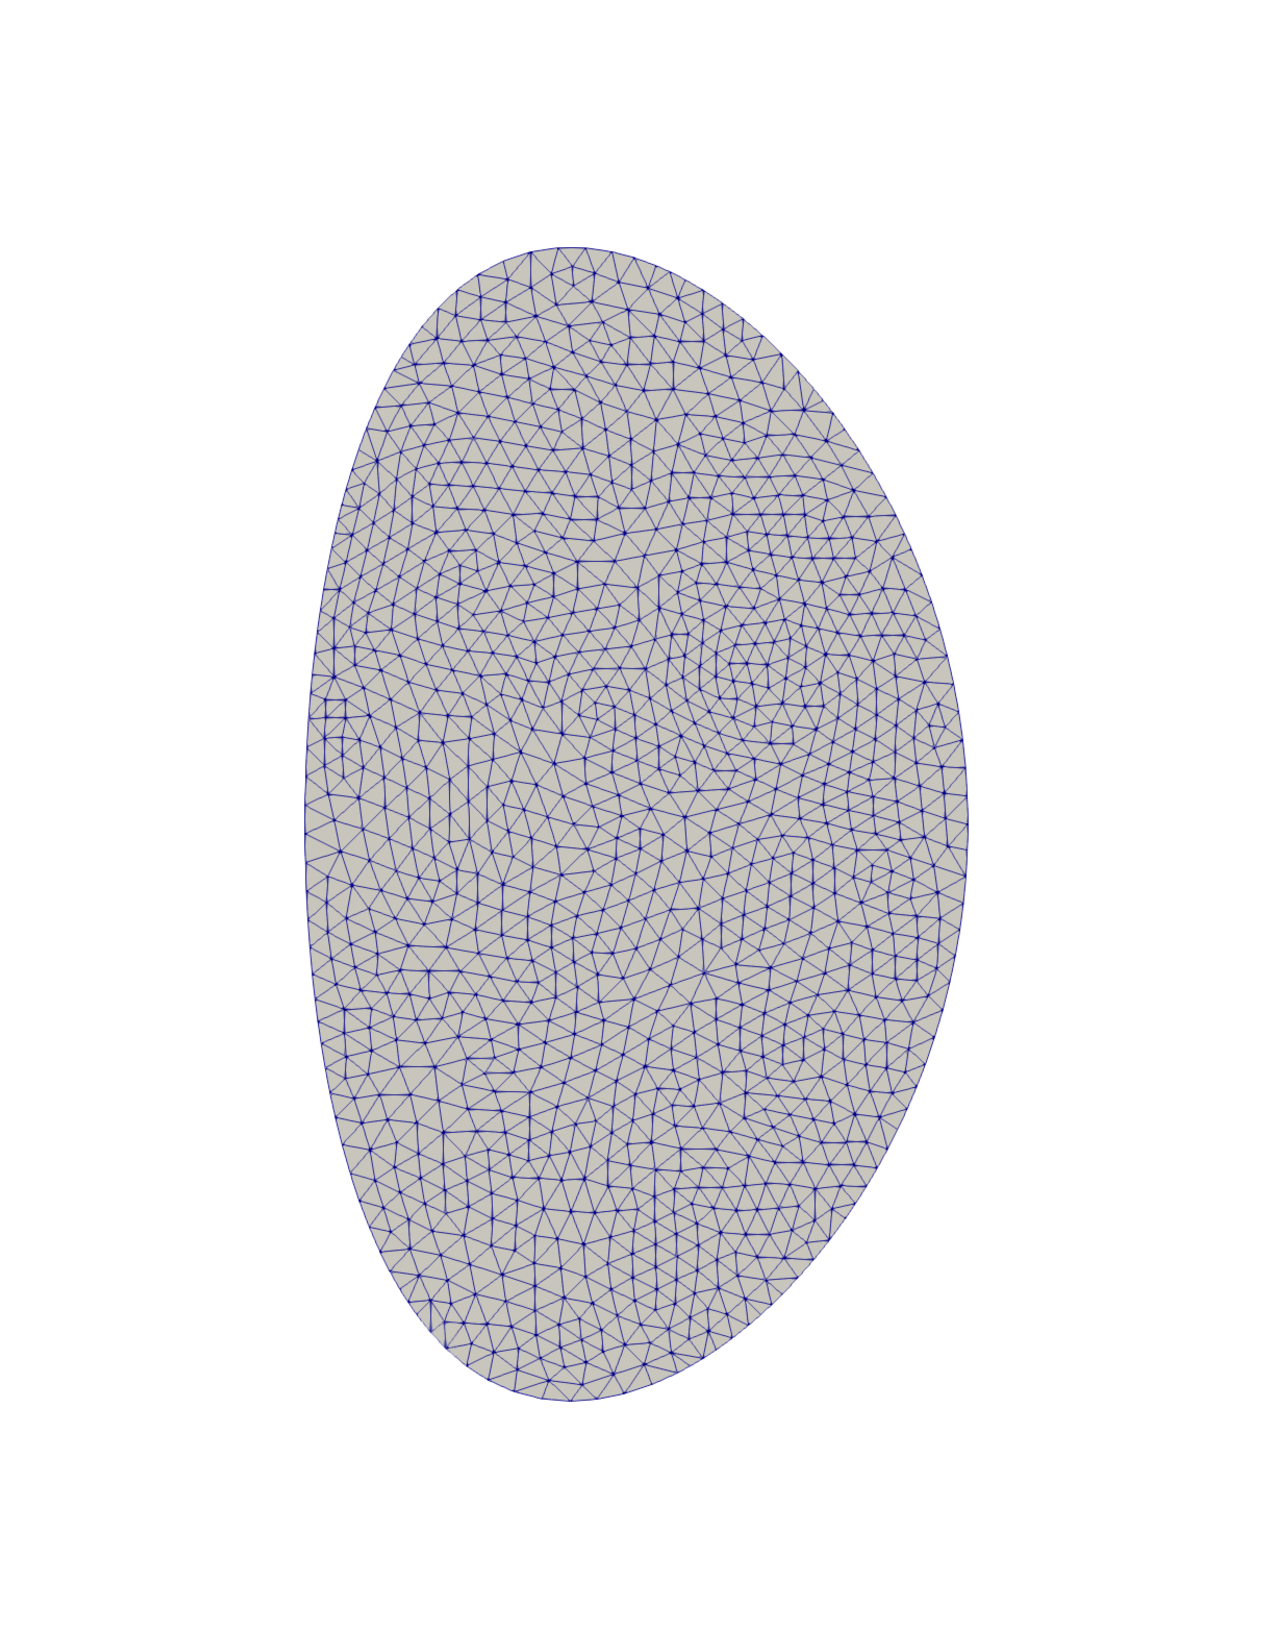
\includegraphics[width=3in]{./figures/meshgen-type0.pdf}
\caption[Mesh with vacuum region defined by five parameters for analytic expression]
{A mesh with vacuum region defined by five parameters for analytic expression}
\label{fig:meshgen-type0}
\end{figure}

The figure~\ref{fig:meshgen-type0} illustrates a mesh generated by the following input file.

\begin{verbatim}
modelType 0
outFile analytic 
meshSize 0.04

useVacuumParams 1
vacuumParams 1.65908 0.46 0.2 -0.02504 0.8
numVacuumPts 20

adjustVacuumParams 0
vacuumFactor  6.28319
\end{verbatim}

\begin{figure}
\centering
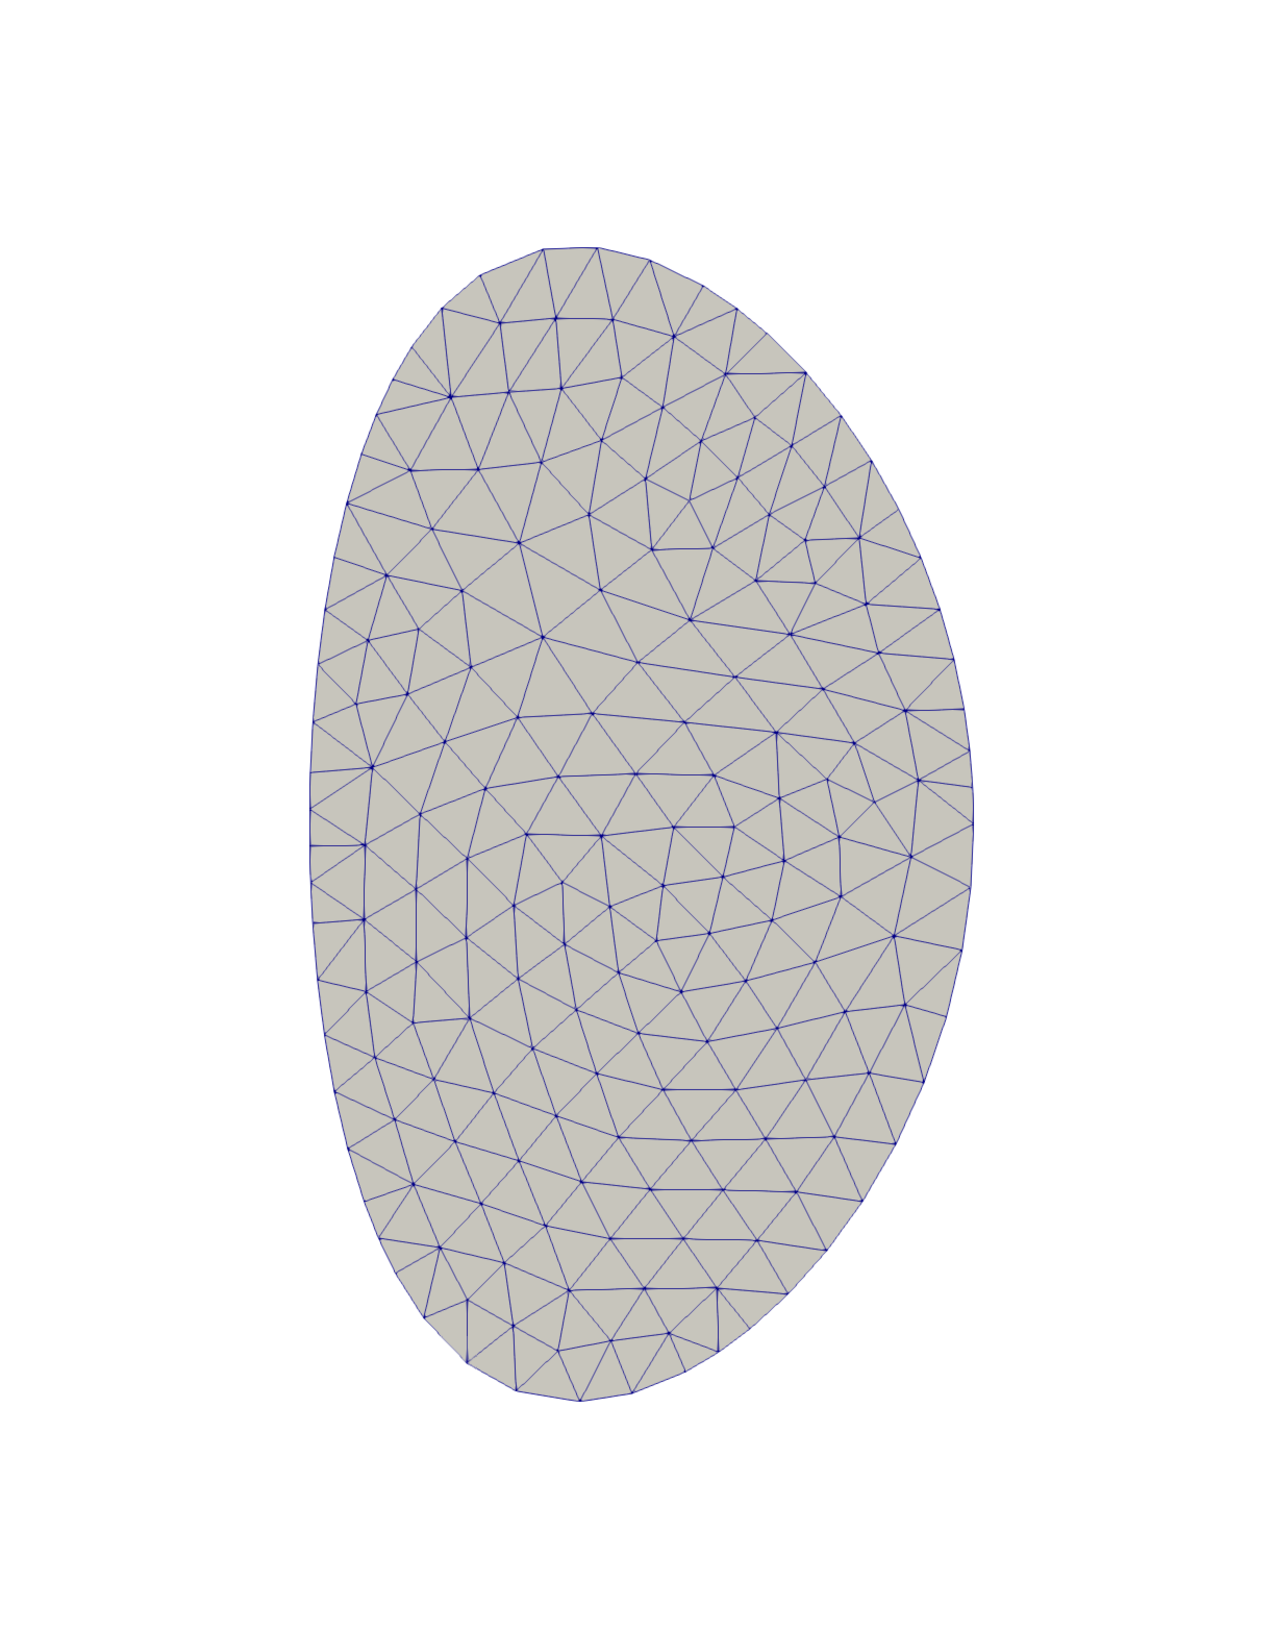
\includegraphics[width=3in]{./figures/meshgen-type0-ms.pdf}
\caption[Mesh generated with vacuum region parameters and mesh size 0.1]
{A mesh generated with vacuum region parameters and mesh size 0.1}
\label{fig:meshgen-type0-ms}
\end{figure}

The figure~\ref{fig:meshgen-type0-ms} illustrates a mesh generated with the same vacuum region parameters and a higher mesh size value.

%%%%%%%%%%%%%%%%%%%%%%%%%%%%%%%%%%%%%%%%%
\subsubsection{Type 2 (piece-wise polynomial vacuum)}
%%%%%%%%%%%%%%%%%%%%%%%%%%%%%%%%%%%%%%%%%

\begin{figure}
\centering
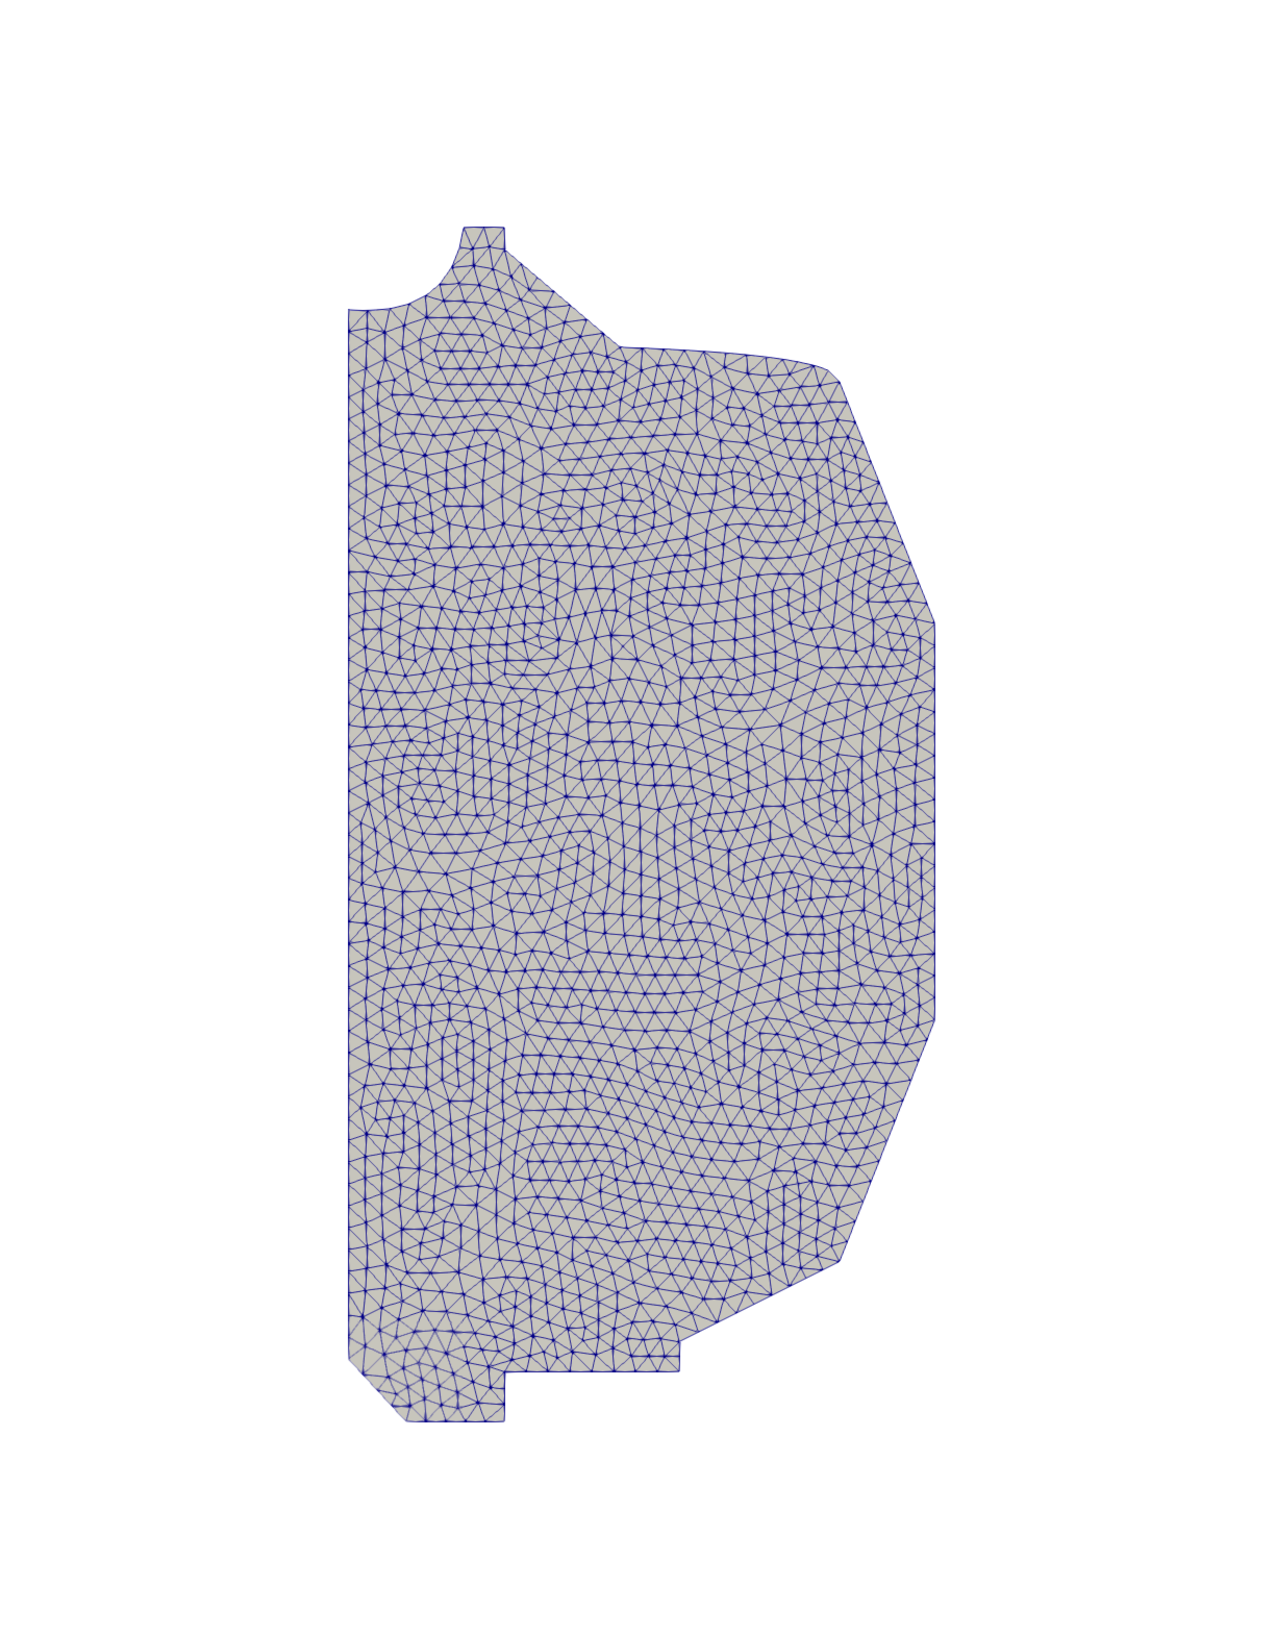
\includegraphics[width=3in]{./figures/meshgen-type2.pdf}
\caption[Mesh with vacuum region defined by piece-wise polynomials]
{A mesh with vacuum region defined by piece-wise polynomials}
\label{fig:meshgen-type2}
\end{figure}

The figure~\ref{fig:meshgen-type2} illustrates a mesh generated by the following input file. The vacuum region's geometry information is defined by piece-wise polynomials and stored in the file \texttt{in-poly}. 

\begin{verbatim}
modelType 2
inFile in-poly
outFile poly
\end{verbatim}

The vacuum region's geometry information is defined by piece-wise polynomials and stored in the file \texttt{in-poly} and the example file can be found in 
\newline\newline
\texttt{/p/tsc/m3dc1/lib/SCORECLib/rhel7/intel2019u3-openmpi4.0.3/16.0-220226/bin}.

%%%%%%%%%%%%%%%%%%%%%%%%%%%%%%%%%%%%%%%%%
\subsubsection{Type 3 (three-regions with inner wall points)}
%%%%%%%%%%%%%%%%%%%%%%%%%%%%%%%%%%%%%%%%%
With the model type 3, a geometric model consists of three model faces where each represents plasma region, resistive region and vacuum region, respectively. An ascii file name which describes inner plasma wall boundary has to be provied with the parameter \texttt{inFile}.

\begin{figure}
\centering
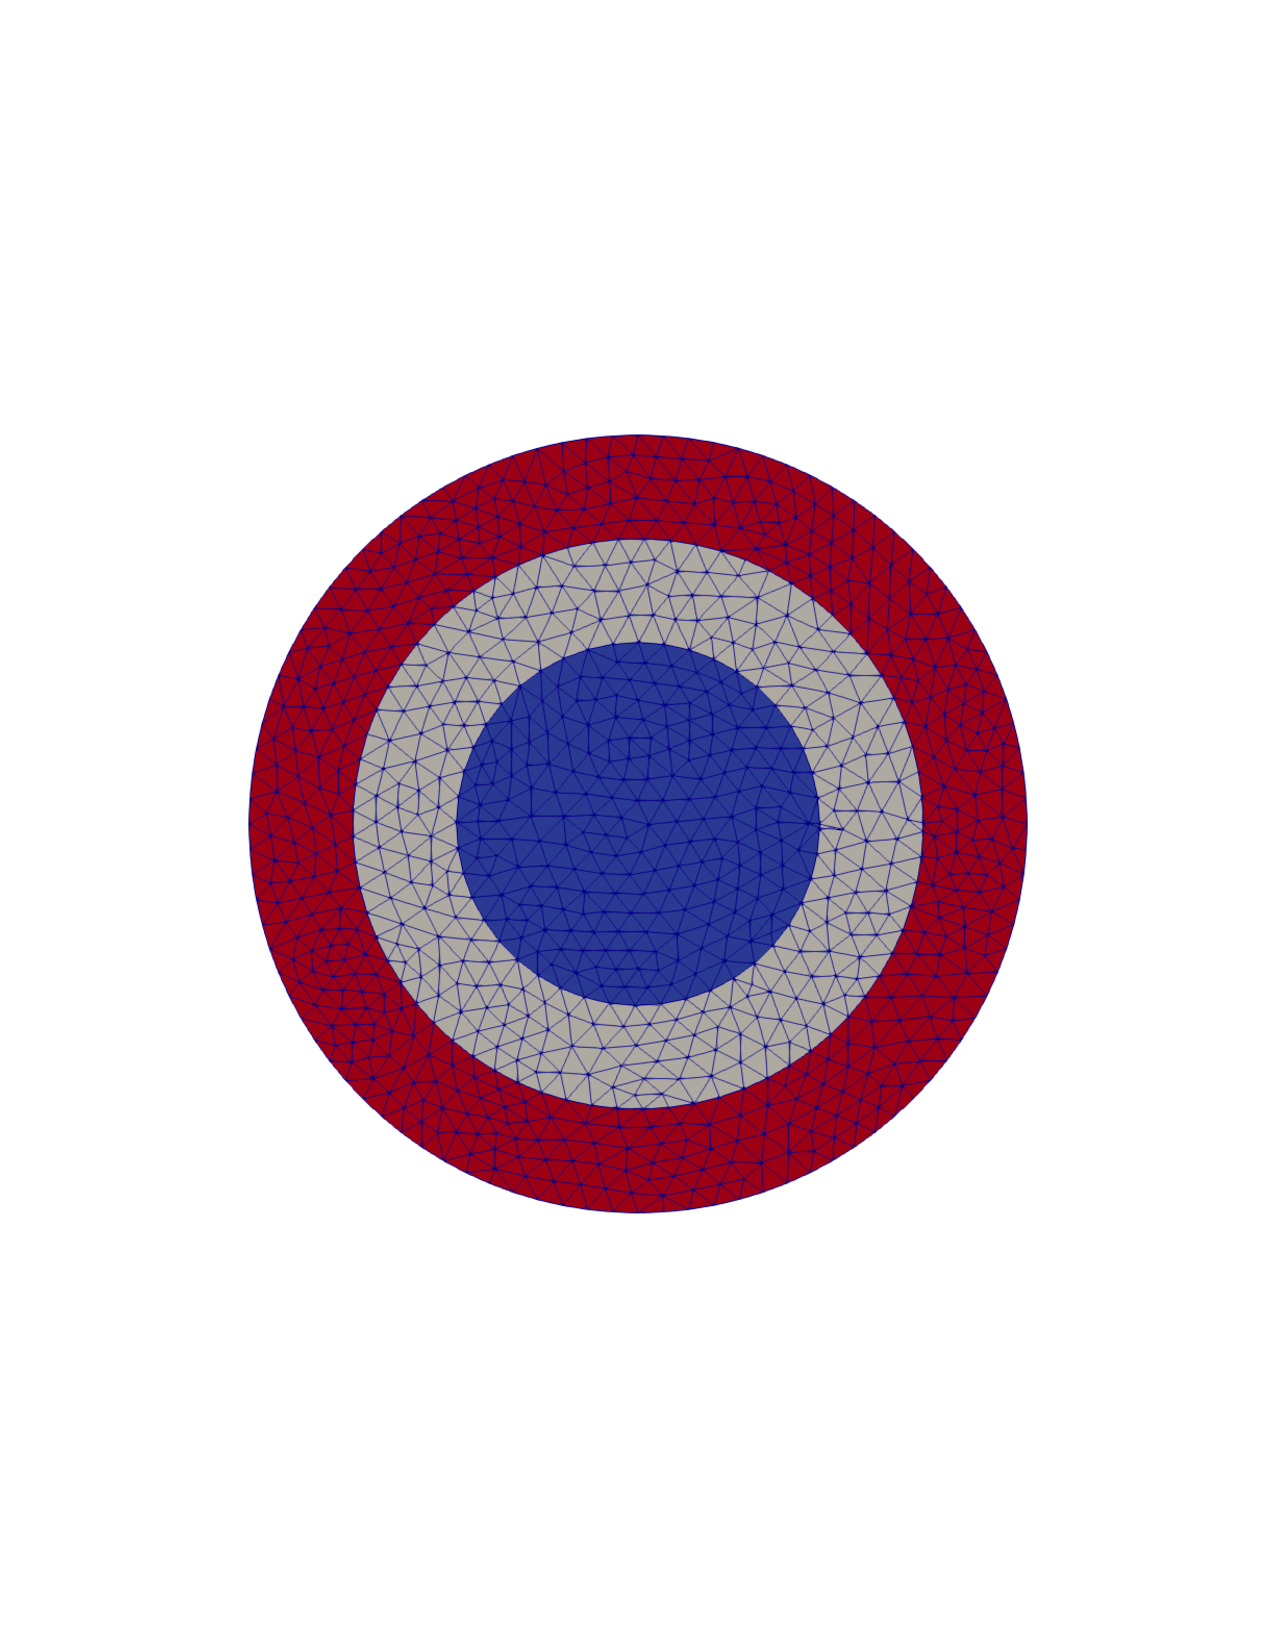
\includegraphics[width=3in]{./figures/meshgen-type3.pdf}
\caption[Mesh with spline-fitted 3-region model]
{A mesh with spline-fitted 3-region model}
\label{fig:meshgen-type3}
\end{figure}

The figure~\ref{fig:meshgen-type3} illustrates a mesh generated by the following input file. In the figure, geometric model faces are different colored.

\begin{verbatim}
modelType 3
inFile in-circle
outFile circle
meshSize 0.1 0.5 0.1
useVacuumParams 1
adjustVacuumParams 1
vacuumParams 5.0 1.5 0.0 0.0 1.5
numVacuumPts 20
meshGradationRate 0.4
resistive-width 0.4
\end{verbatim}

The example files \texttt{circle-input} and \texttt{in-circle} can be found in
\newline\newline
\texttt{/p/tsc/m3dc1/lib/SCORECLib/rhel7/intel2019u3-openmpi4.0.3/16.0-220226/bin}.

%%%%%%%%%%%%%%%%%%%%%%%%%%%%%%%%%%%%%%%%%
\subsubsection{Type 4 (three-regions with inner $\&$ outer wall points)}
%%%%%%%%%%%%%%%%%%%%%%%%%%%%%%%%%%%%%%%%%

With the model type 4, a geometric model consists of three model faces where each represents plasma region, resistive region and vacuum region, respectively.  The parameter \texttt{inFile} denotes a file name that contains inner plasma wall boundary. The parameter \texttt{bdryFile} denotes a file name that contains resistive wall boundary.

\begin{figure}
\centering
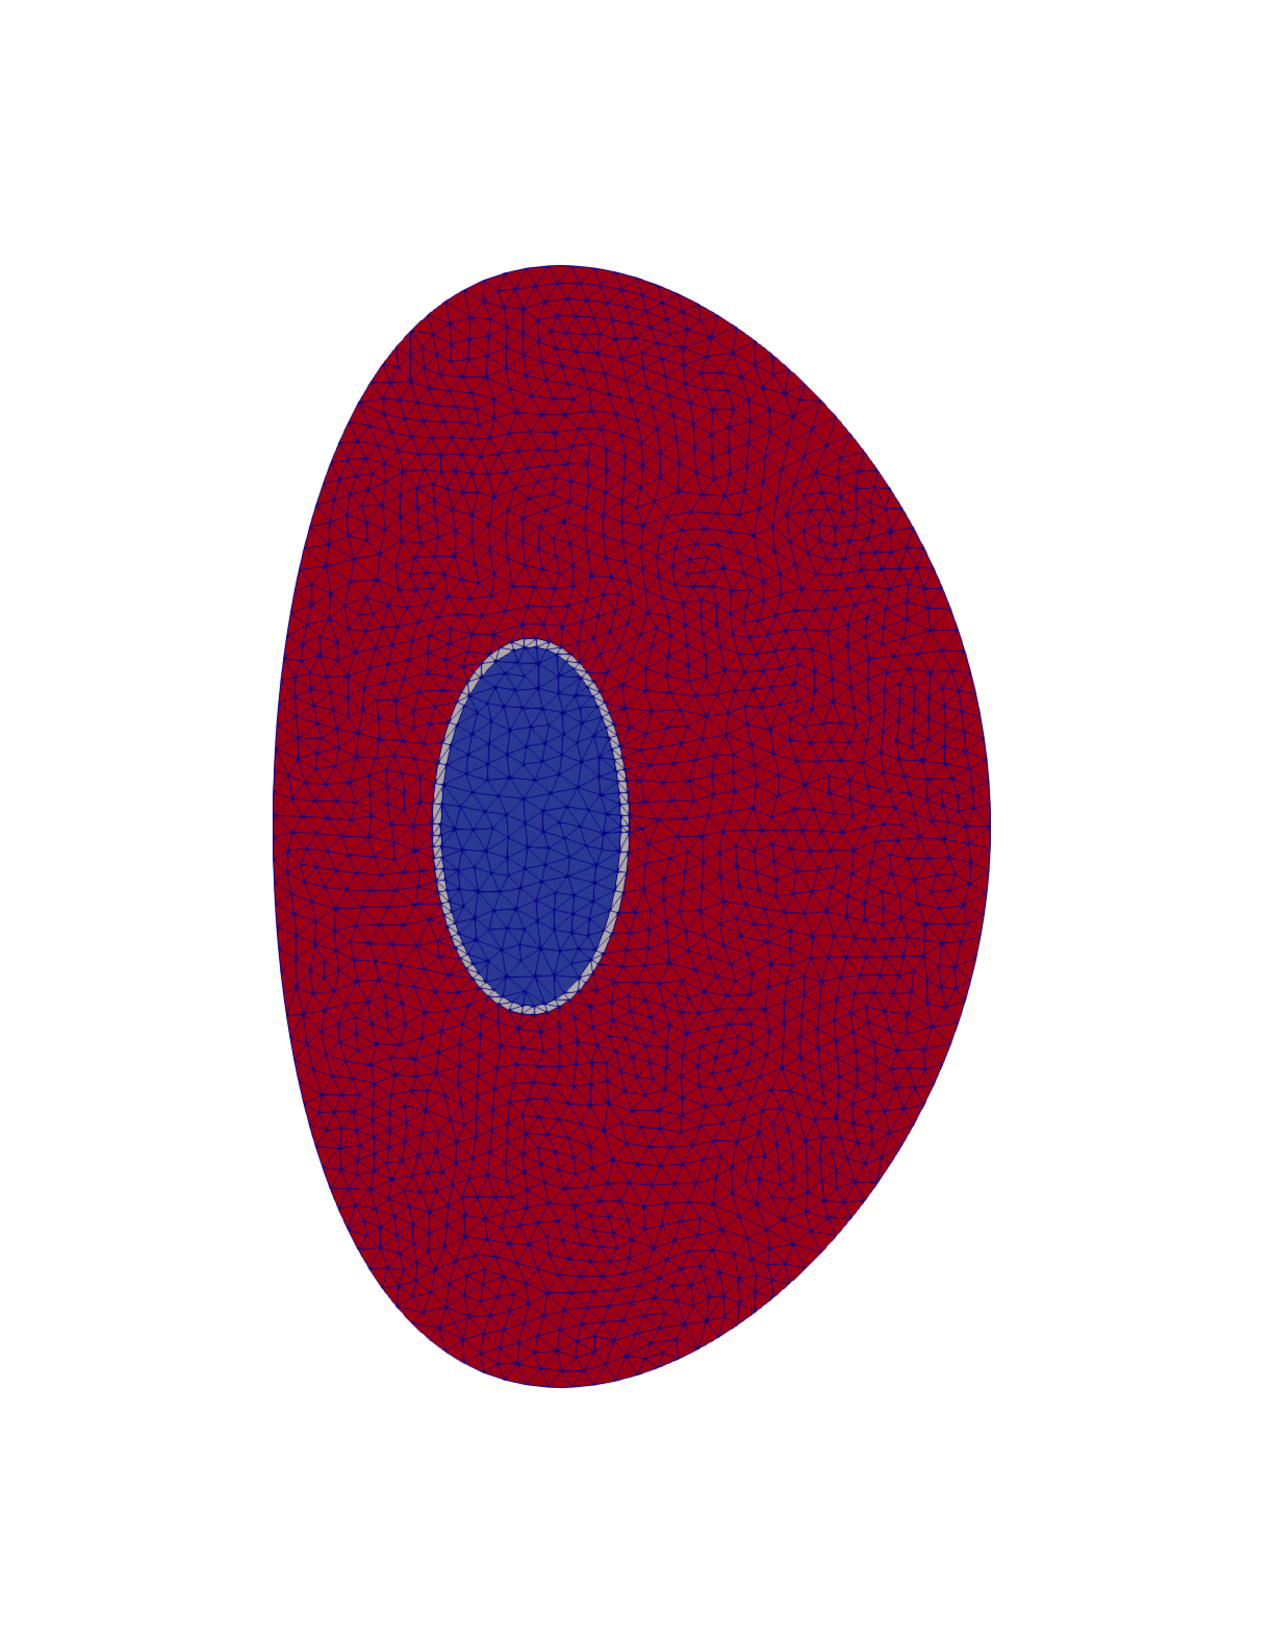
\includegraphics[width=3in]{./figures/meshgen-type4.pdf}
\caption[Mesh with inner $\&$ outer plasma wall boundary points]
{A mesh with inner $\&$ outer plama wall boundary points}
\label{fig:meshgen-type4}
\end{figure}

The figure~\ref{fig:meshgen-type4} illustrates a mesh generated by the following input file. In the figure, geometric model faces are different colored.

\begin{verbatim}
modelType 4
inFile inner_bdry.pts
bdryFile outer_bdry.pts
outFile iter
meshSize 0.7 0.5 0.7
useVacuumParams 1
adjustVacuumParams 1
vacuumParams 8.25 8.0 0.2 0.0 12.5
meshGradationRate 1
\end{verbatim}

The example files \texttt{bdry-input}, \texttt{inner\_bdry.pts} and \texttt{outer\_bdry.pts} can be found in
\newline\newline
\texttt{/p/tsc/m3dc1/lib/SCORECLib/rhel7/intel2019u3-openmpi4.0.3/16.0-220226/bin}.

%%%%%%%%%%%%%%%%%%%%%%%%%%%%%%%%%%%%%%%%%
\subsection{m3dc1\_mfmgen}
\label{ch:mfm-gen}
%%%%%%%%%%%%%%%%%%%%%%%%%%%%%%%%%%%%%%%%%

\texttt{m3dc1\_mfmgen} requires an ascii input file of arbitrary name that contains the following parameters.
The parameters can be in any order.

\begin{itemize}
\item numBdry: the number of boundary files defined by peice-wise linear points given for the construction of the loops (default: 0)
  \begin{itemize}
  \item Each boundary file corresponds to a loop in PUMI
  \item For \texttt{numBdry}=$N$, $N$ lines of \texttt{bdryFile} should be provided, $N \ge 0$
  \end{itemize}
\item bdryFile: For each boundary file, the user has to provide its file name followed by the unique loop ID and desired mesh size on the loop.
  \begin{itemize}
  \item Each boundary file corresponds to a loop in PUMI
  \item The unique ID can be an arbitrary integer defined by the user
  \item The unique ID is used with input parameter ``faceBdry" to specify the boundaries (loops) of model face
  \item For more than one boundary files (numBdry$>$1), the boundary files can be in any order
  \end{itemize}

\item useVacuum: A parameter to control the vacuum boundary
  \begin{itemize}
  \item The first number sets the mode of vacuum boundary and can be 0, 1 or 2. If 0, no vacuum boundary will be created. If 1, vacuum boundary will be created without user defined parameters. If 2, a parameterized vacuum boundary will be created by using the parameters defined in the parameter "vacuumParams".
  \item The second number is the desired unique loop ID for the vacuum loop
  \item  The third number defines the mesh size on the vacuum boundary
  \end{itemize}
\item vacuumParams: if ``useVacuum = 2", the user has to provide five doubles to define parameterized vacuum wall
\item numVacuumPts: if ``useVacuum = 2", \# interpolation points on parameterized vacuum wall (default=20)

\item thickWall: three integers and one double to control finite thickness wall
  \begin{itemize}
  \item The first number can either be 0 or 1. If it is set to 0, no finite thickness wall will be created. If it is set to 1, a finite thickness wall will be created
  \item The second number is the loop ID that will be offset for given thickness
  \item The third number is the desired unique loop ID for the new loop created from offsetting for the finite thickness wall
  \item The last number is the desired wall thickness
  \end{itemize} 

\item layeredMesh: two integers to create an extruded layeded mesh on the finite thickness wall
  \begin{itemize}
  \item The first integer is 0, no layered mesh will be created. If 1 (default), an extruded mesh with desired number of mesh layers will be created
  \item The second integer defines the number of mesh layers
  \end{itemize}

\item numFace: the number of geometric model faces in PUMI (default 1)
    \begin{itemize}
  \item Each geometric face corresponds to regions (e.g. plasma, resistive, vacuum) in M3DC1
  \item For \texttt{numFace}=$N$, $N$ lines of \texttt{faceBdry} should be provided, $N > 0$
  \end{itemize}
\item faceBdry: For each model face, the user has to provide the number of loops, loop ID(s), and desired mesh size
  \begin{itemize}
  \item The first number gives the total number of loops bounding the face
  \item the first number is followed by the loops IDs of the bounding loops. If number of loops = $n$, there should be $n$ loop ID
  \item The last number is the desired mesh size on the geometric face
    \end{itemize}

\item meshGradationRate: Global mesh gradation rate for the meshing. This parameter is optional and if not specified a default mesh gradation rate = 0.3 is used. This value should be greater than or equal to 0.3. Otherwise the mesh will be fine everywhere.
\item outFile: output file name to save model and mesh
\end{itemize}

Locate input parameter file and all files listed as bdryFile (if applicable) in the work folder and do \texttt{m3dc1\_mfmgen input\_param\_file}. The output files are the same as those of \texttt{m3dc1\_meshgen}.

%%%%%%%%%%%%%%%%%%%%%%%%%%%%%%%%%%%%%%%%%
\subsubsection{Mesh with parameterized vacuum wall}
%%%%%%%%%%%%%%%%%%%%%%%%%%%%%%%%%%%%%%%%%

This section presents a mesh created with a parameterized vacuum wall. This is equivalent to \texttt{Type 0} mesh of \texttt{m3dc1\_meshgen}.

\begin{verbatim}
numBdry 0
useVacuum 1 1 0.1
numFace 1
faceBdry 1 1 0.09
outFile analytic-0.09
\end{verbatim}

\begin{figure}
\centering
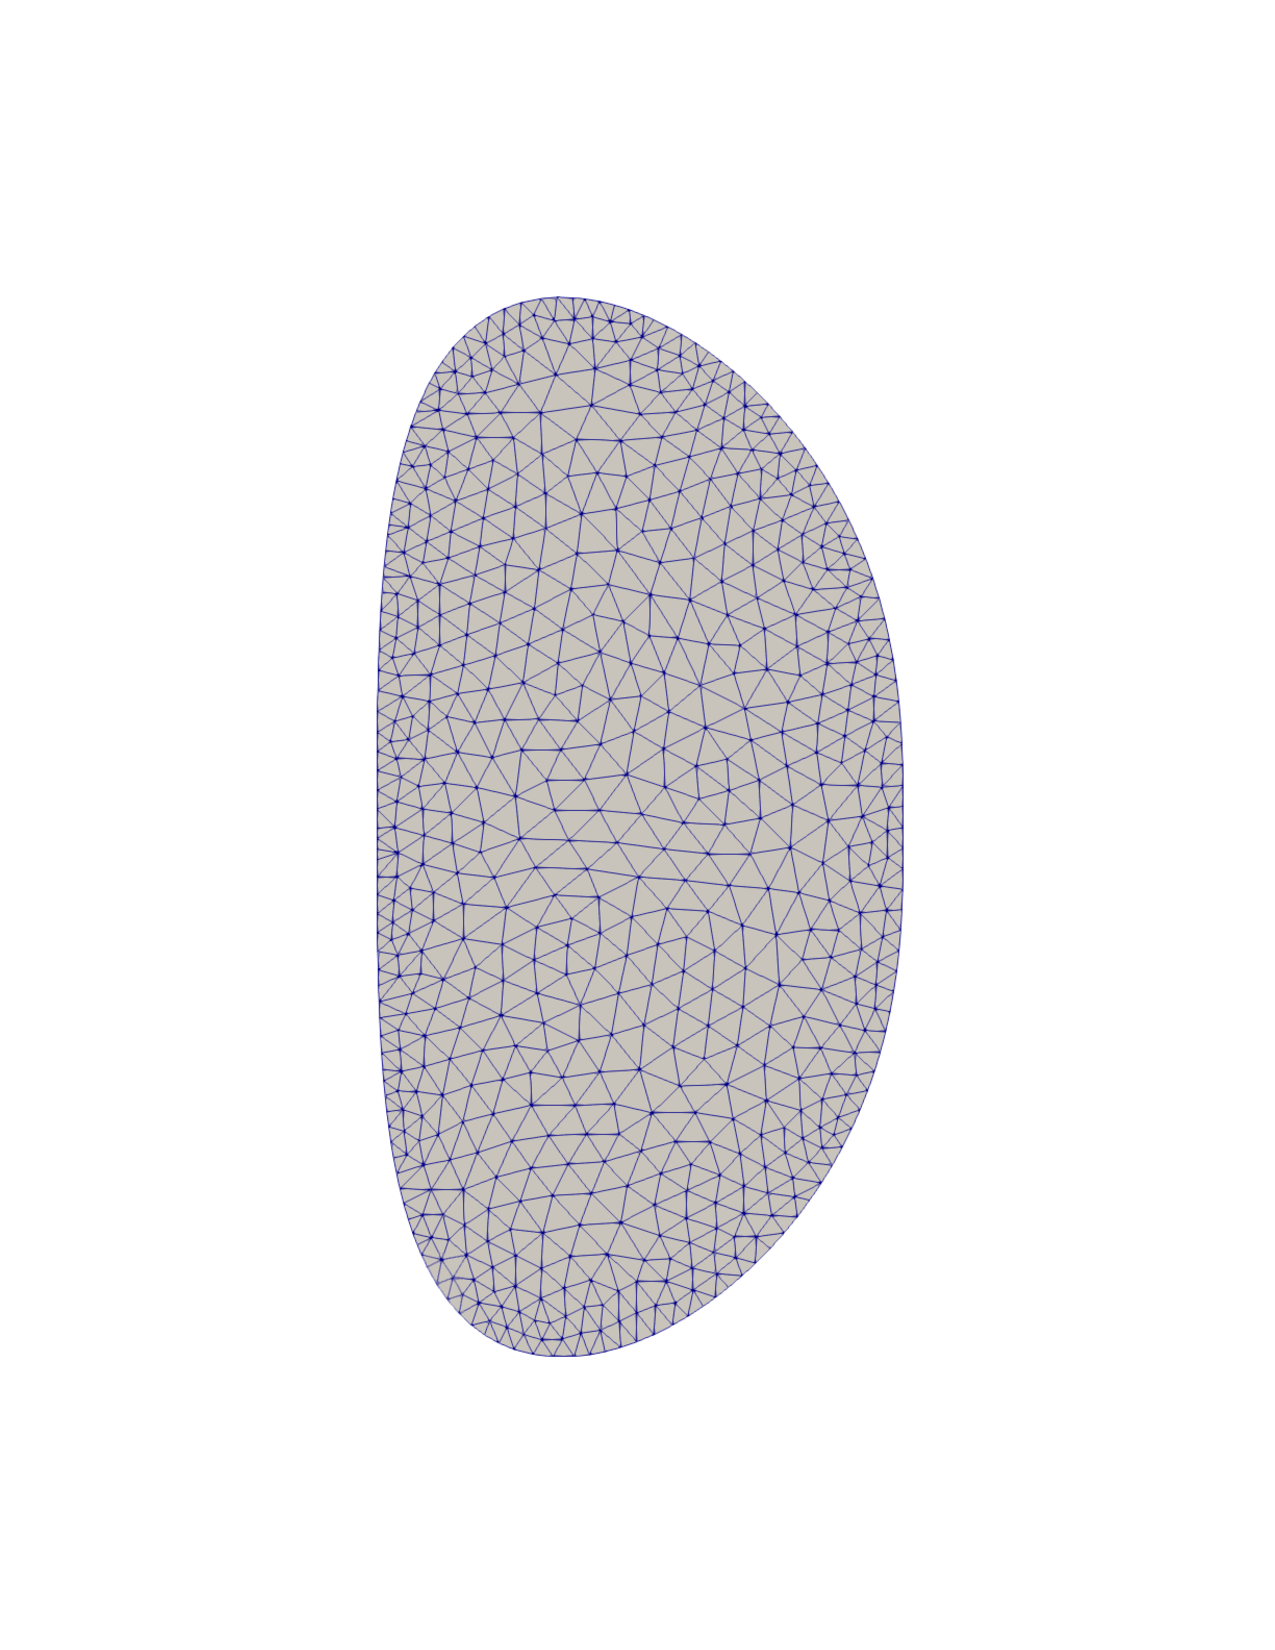
\includegraphics[width=3in]{./figures/meshgen-analytic-20pts-05.pdf}
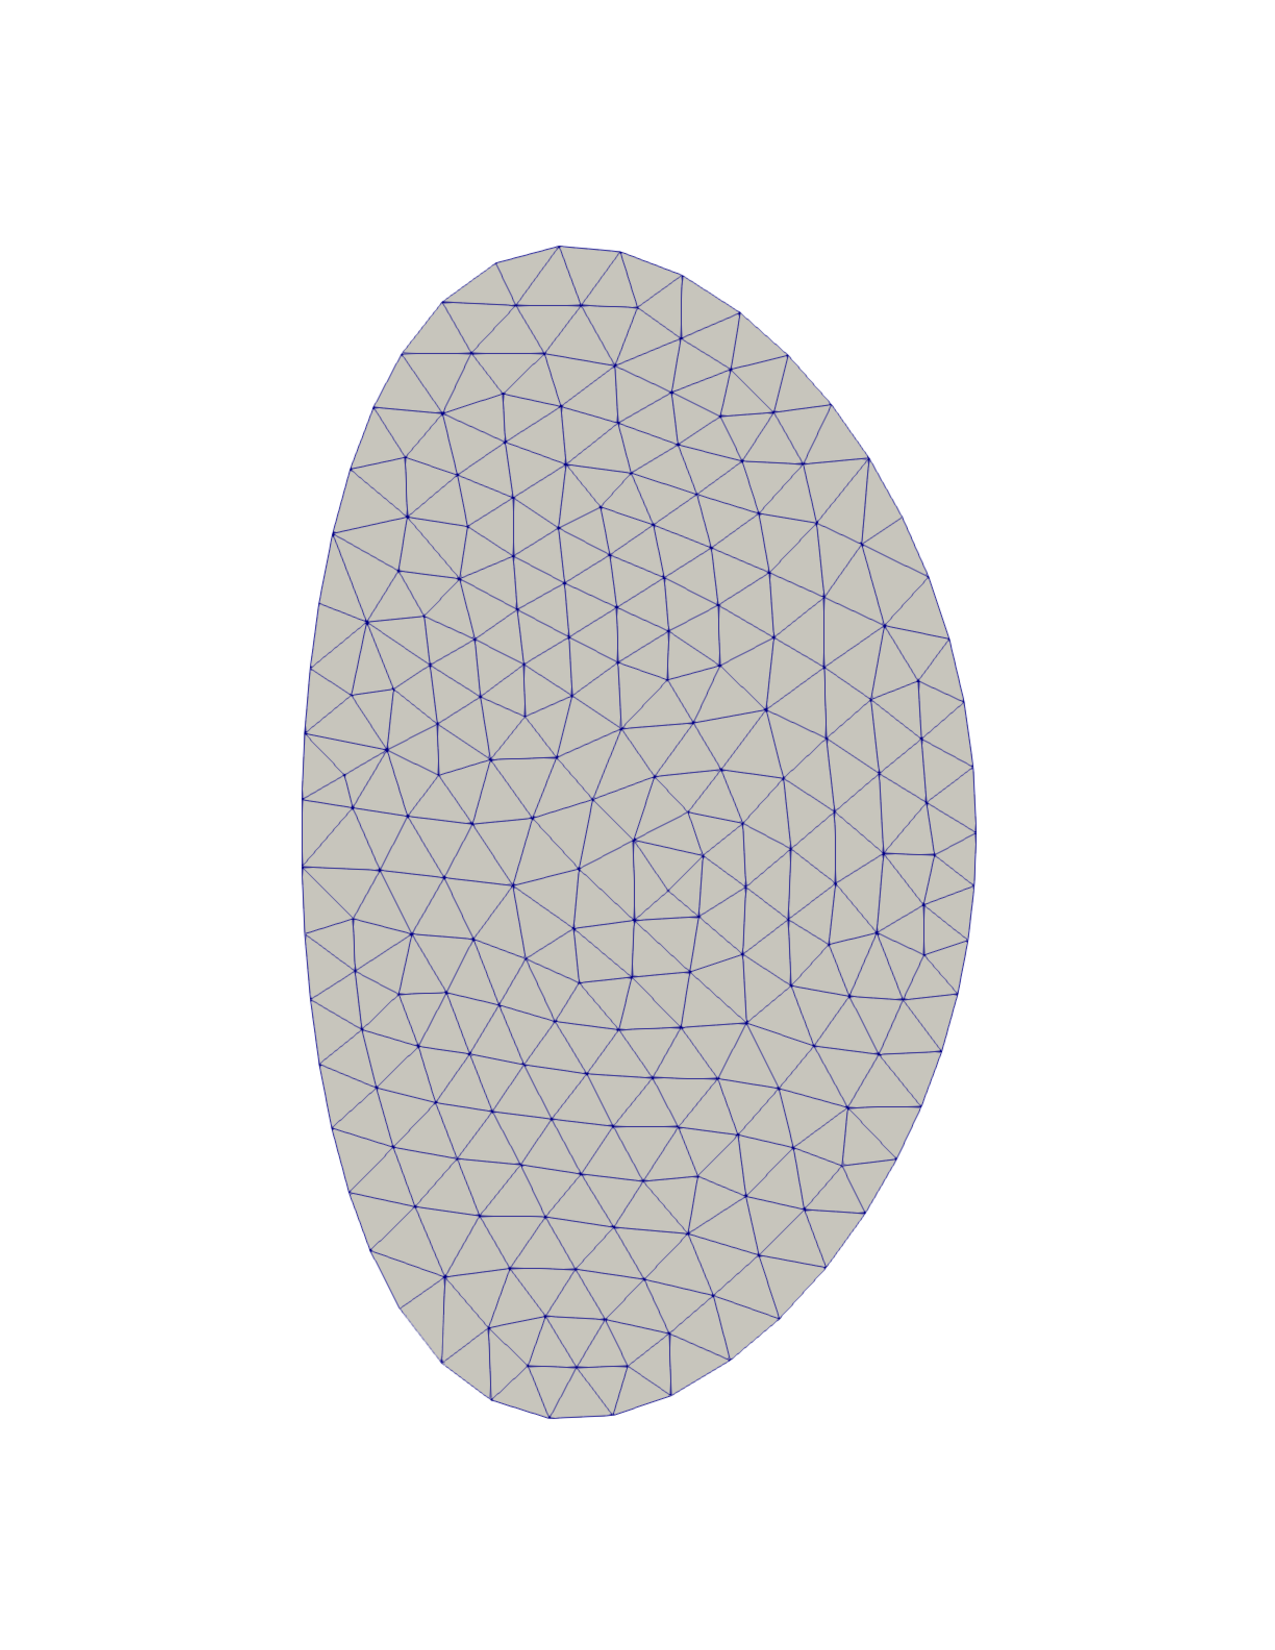
\includegraphics[width=3in]{./figures/meshgen-analytic-20pts-09.pdf}
\caption{Mesh with a parameterized vacuum region and different mesh size for model face (left) 0.2 (right) 0.09}
\label{fig:analytic-mesh}
\end{figure}

The figure~\ref{fig:analytic-mesh} presents the mesh generated by the input file above with two different mesh sizes.

%\begin{verbatim}
%numBdry 0
%numFace 1
%faceBdry 1 1
%outFile analytic-0.05
%meshSize 0.05
%useVacuumParams 1
%vacuumParams 1.65908 0.46 0.2 -0.02504 0.8
%numVacuumPts 50
%\end{verbatim}

%\begin{figure}
%\centering
%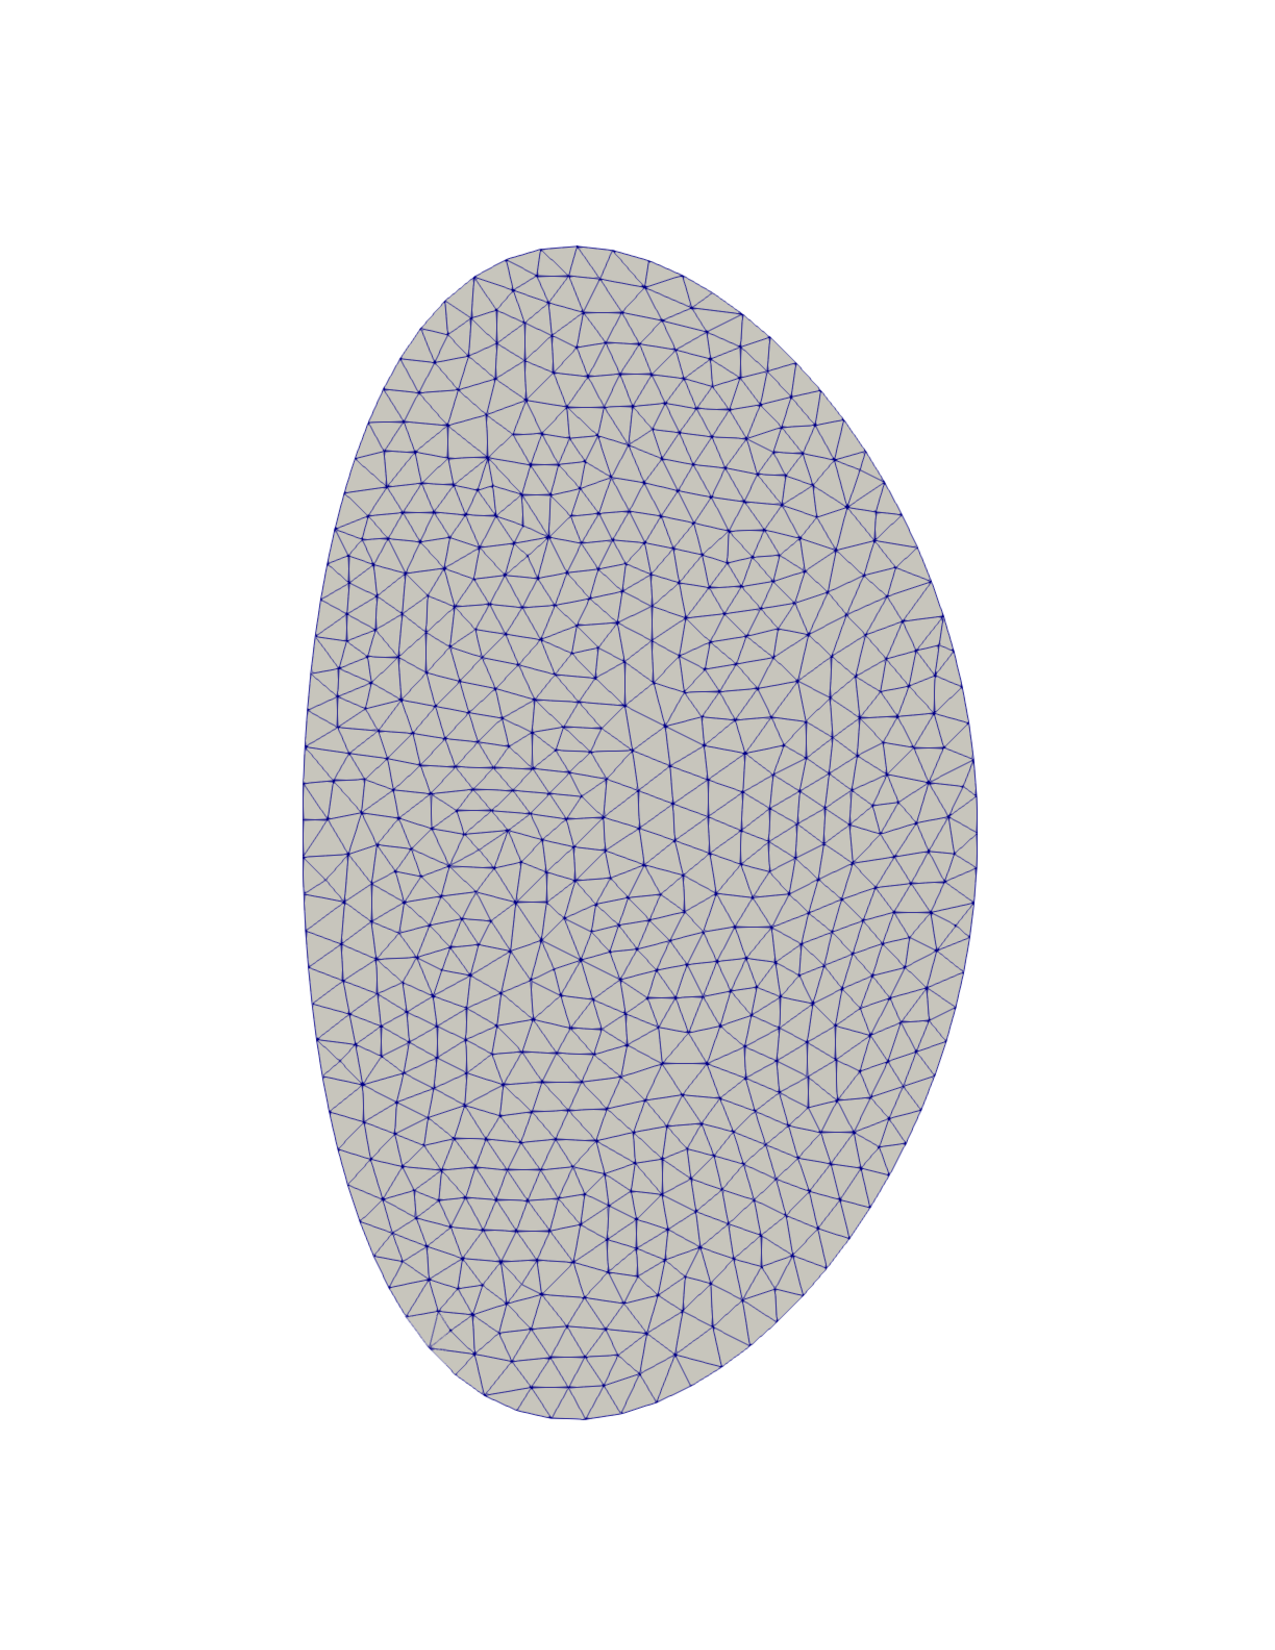
\includegraphics[width=3in]{./figures/meshgen-analytic-50pts-05.pdf}
%\caption[Mesh with parameterized vacuum region II]
%{A mesh with parameterized vacuum region of 50 interpolation points and mesh size 0.05}
%\label{fig:analytic-mesh-2}
%\end{figure}
%
%The figure~\ref{fig:analytic-mesh-2} presents the mesh generated by the input file above.

%%%%%%%%%%%%%%%%%%%%%%%%%%%%%%%%%%%%%%%%%
\subsubsection{Mesh with single boundary file}
%%%%%%%%%%%%%%%%%%%%%%%%%%%%%%%%%%%%%%%%%

\begin{verbatim}
numBdry 1
bdryFile loop1.dat 3 0.1
numFace 1
faceBdry 1 3 0.2
outFile input1
\end{verbatim}

\begin{figure}
\centering
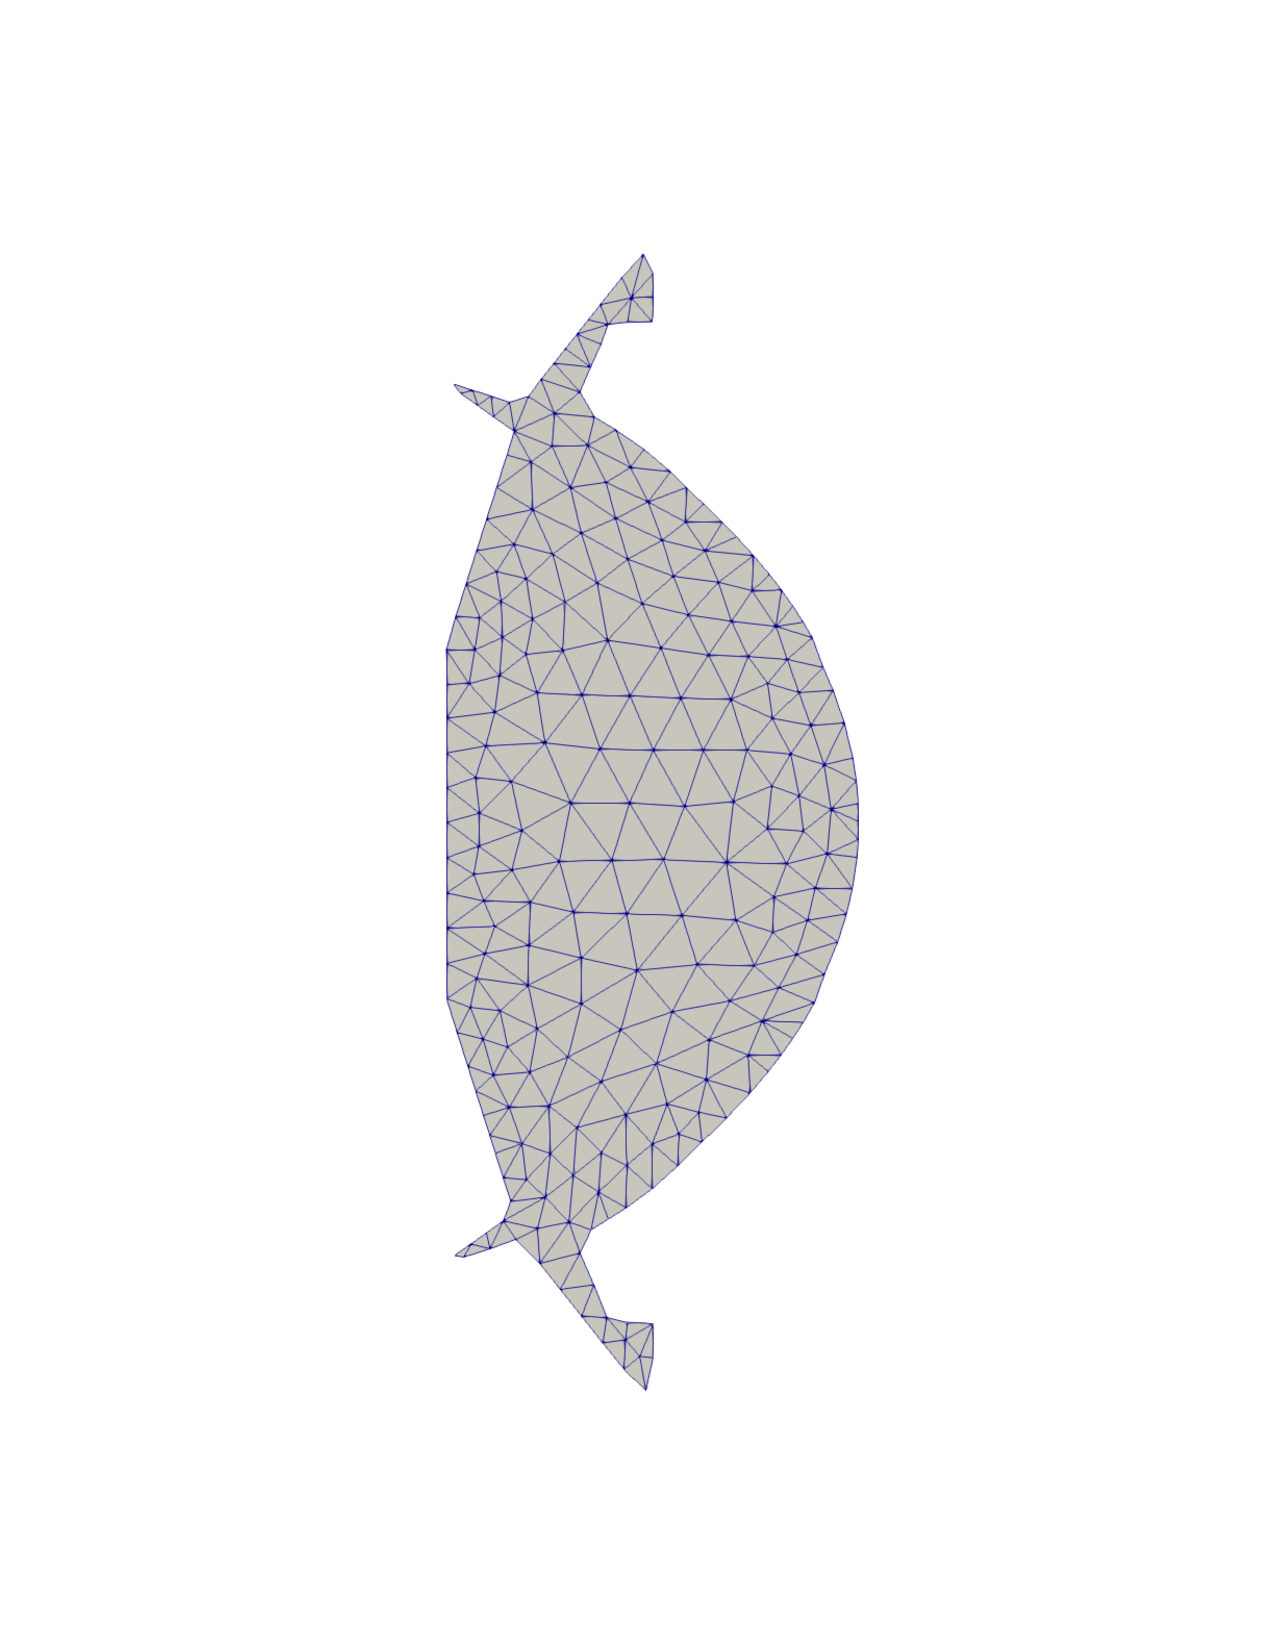
\includegraphics[width=3in]{./figures/meshgen-input1-novacuum.pdf}
\caption{Mesh with single boundary file and no vacuum wall}
\label{fig:input1}
\end{figure}

The figure~\ref{fig:input1} presents the mesh generated by the input file above.

%%%%%%%%%%%%%%%%%%%%%%%%%%%%%%%%%%%%%%%%%
%\subsubsection{Mesh with single boundary file and a vacuum wall} 
%%%%%%%%%%%%%%%%%%%%%%%%%%%%%%%%%%%%%%%%%
%\begin{verbatim}
%numBdry 1
%bdryFile loop1.dat 3 0.1
%
%thickWall 0 19 8 0.07
%useVacuum 2 9 0.01
%vacuumParams 1.8 1.5 0.4 0.0 2.5
%numVacuumPts 20
%
%numFace 1
%faceBdry  1 3 0.2
%outFile input1
%
%meshGradationRate 0.3
%\end{verbatim}
%
%\begin{figure}
%\centering
%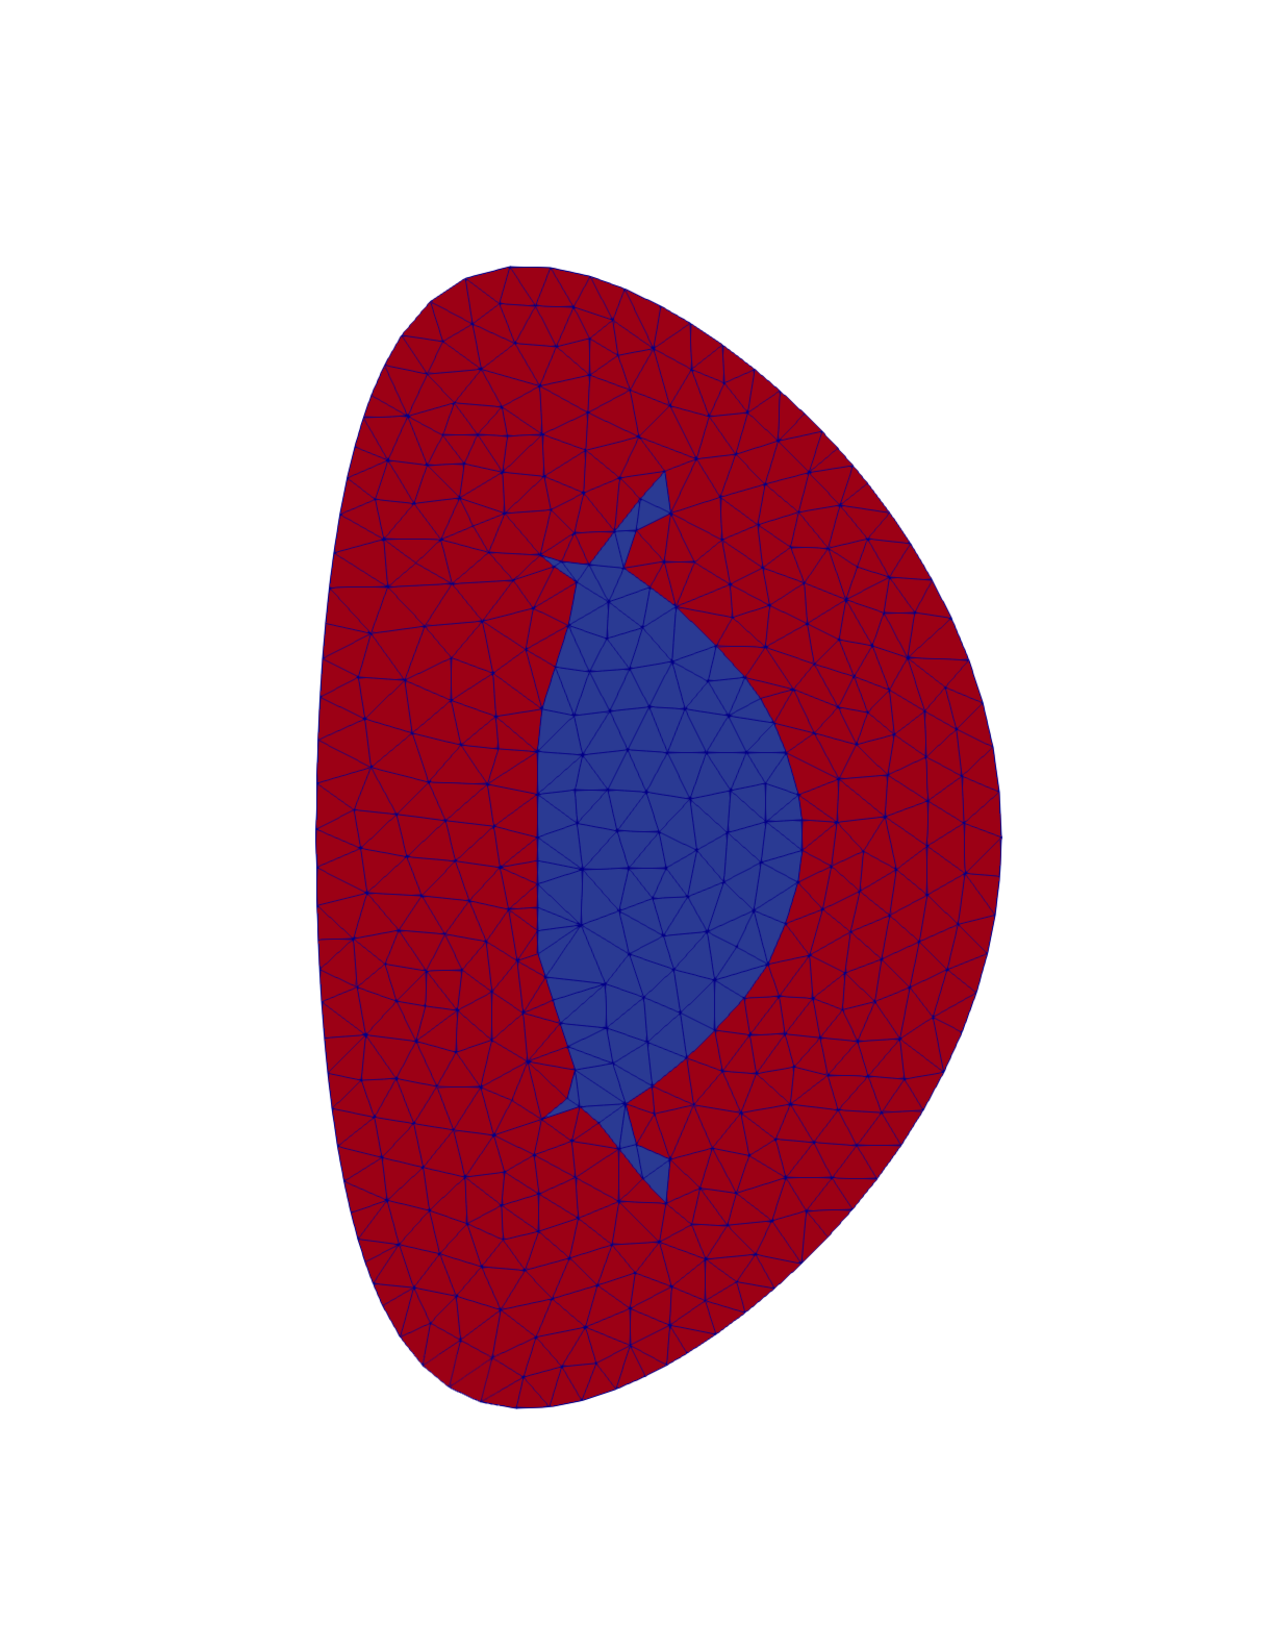
\includegraphics[width=3in]{./figures/meshgen-input1.pdf}
%\caption[Mesh with one boundary file and vacuum wall]
%{Mesh with one boundary file and vacuum wall}
%\label{fig:input1-vacuum}
%\end{figure}

%The figure~\ref{fig:input1-vacuum} presents the mesh generated by the input file above.

%%%%%%%%%%%%%%%%%%%%%%%%%%%%%%%%%%%%%%%%%
\subsubsection{Mesh with two boundary files and a parameterized vacuum wall}
%%%%%%%%%%%%%%%%%%%%%%%%%%%%%%%%%%%%%%%%%

This section presents a mesh created with two boundary files and a parameterized vacuum wall. This is equivalent to \texttt{Type 4} mesh of \texttt{m3dc1\_meshgen}.

\begin{verbatim}
numBdry 2
bddyFile loop1.pts 1 0.5
bdryFile loop2.pts 2 0.5
useVacuum 2 3 0.5
vacuumParams 8.25 8.0 0.2 0.0 12.5
numFace 3
faceBdry 1 1 0.7
faceBdry 2 1 2 0.5
faceBdry 2 2 3 0.7
meshGradationRate 1
outFile iter
\end{verbatim}

\begin{figure}
\centering
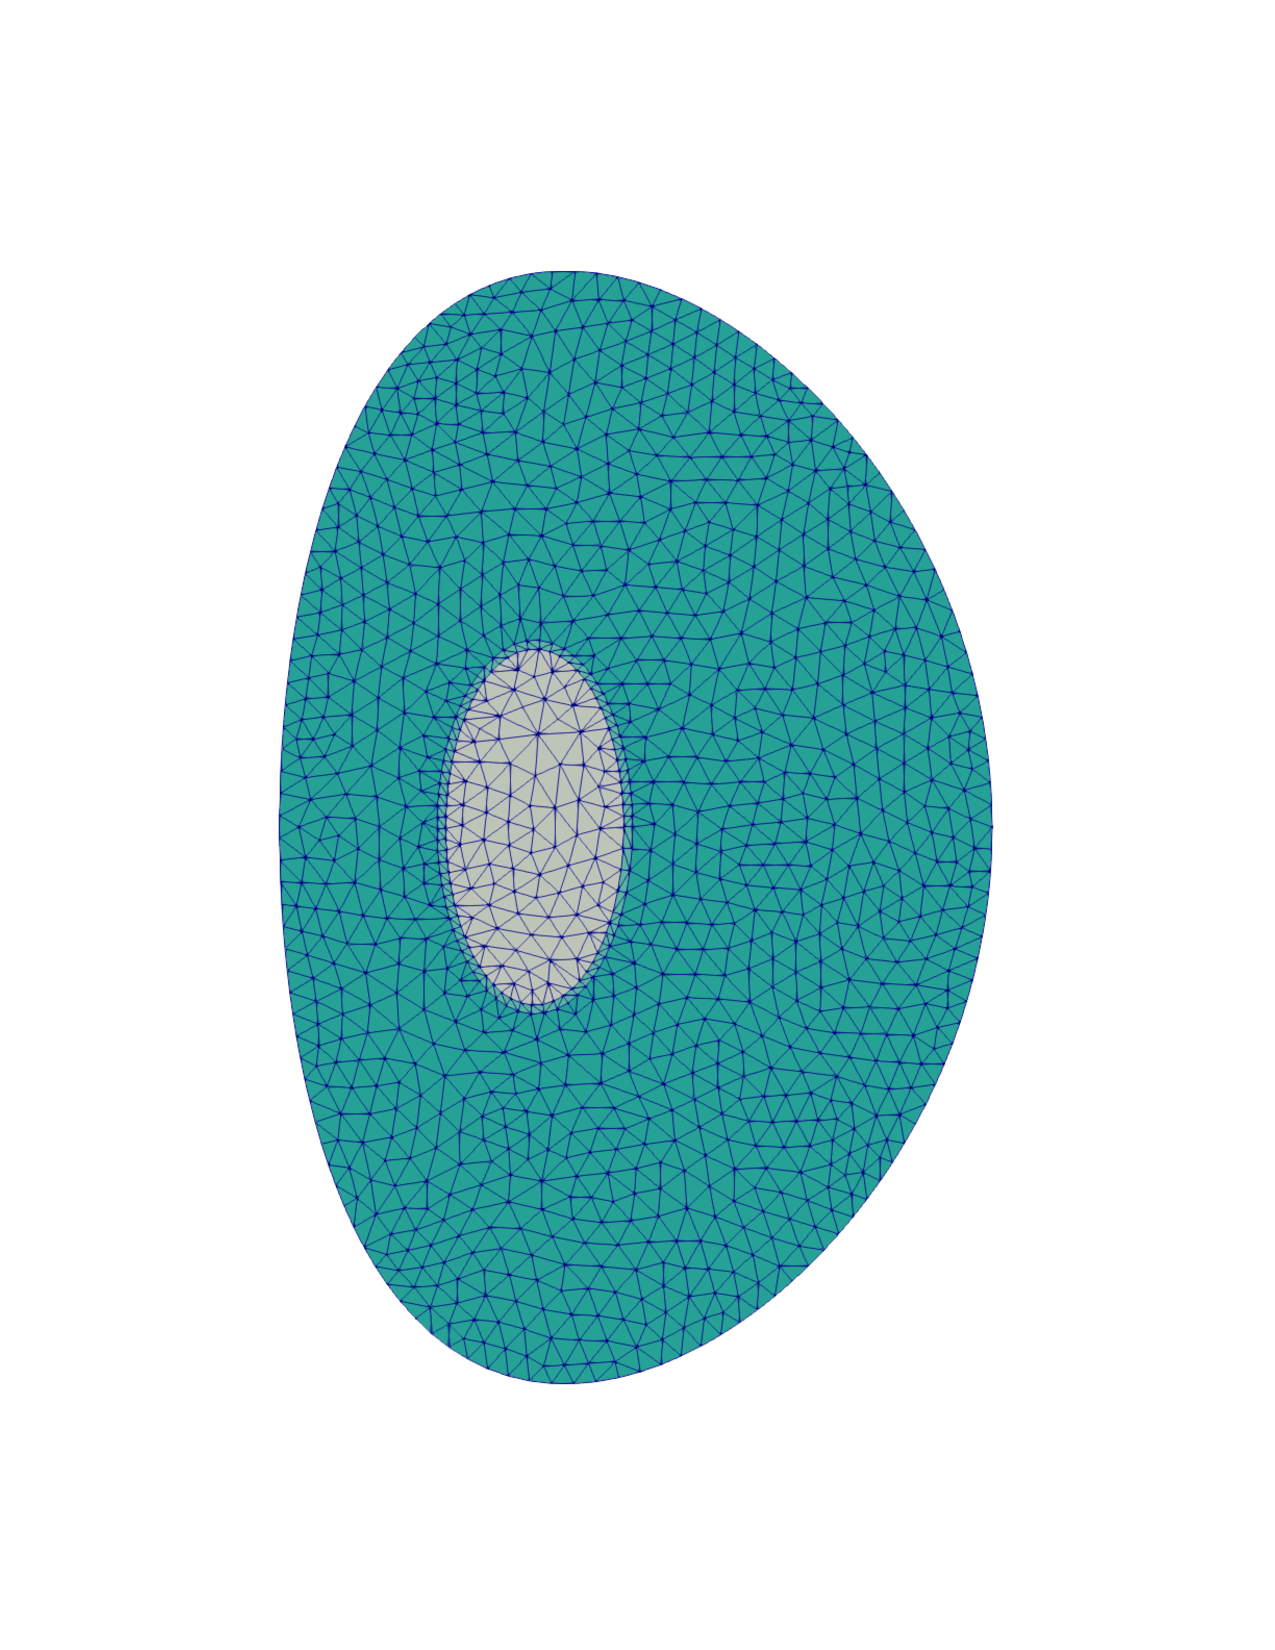
\includegraphics[width=3in]{./figures/meshgen-input2.pdf}
\caption{Mesh with two boundary files and a parameterized vacuum region}
\label{fig:input2}
\end{figure}

The figure~\ref{fig:input2} presents the mesh generated by the input file above. As you can see, the mesh in Figure ~\ref{fig:input2} and ~\ref{fig:meshgen-type4} are almost identical.


%%%%%%%%%%%%%%%%%%%%%%%%%%%%%%%%%%%%%%%%%
\subsubsection{Mesh with three boundary files}
%%%%%%%%%%%%%%%%%%%%%%%%%%%%%%%%%%%%%%%%%

\begin{figure}
\centering
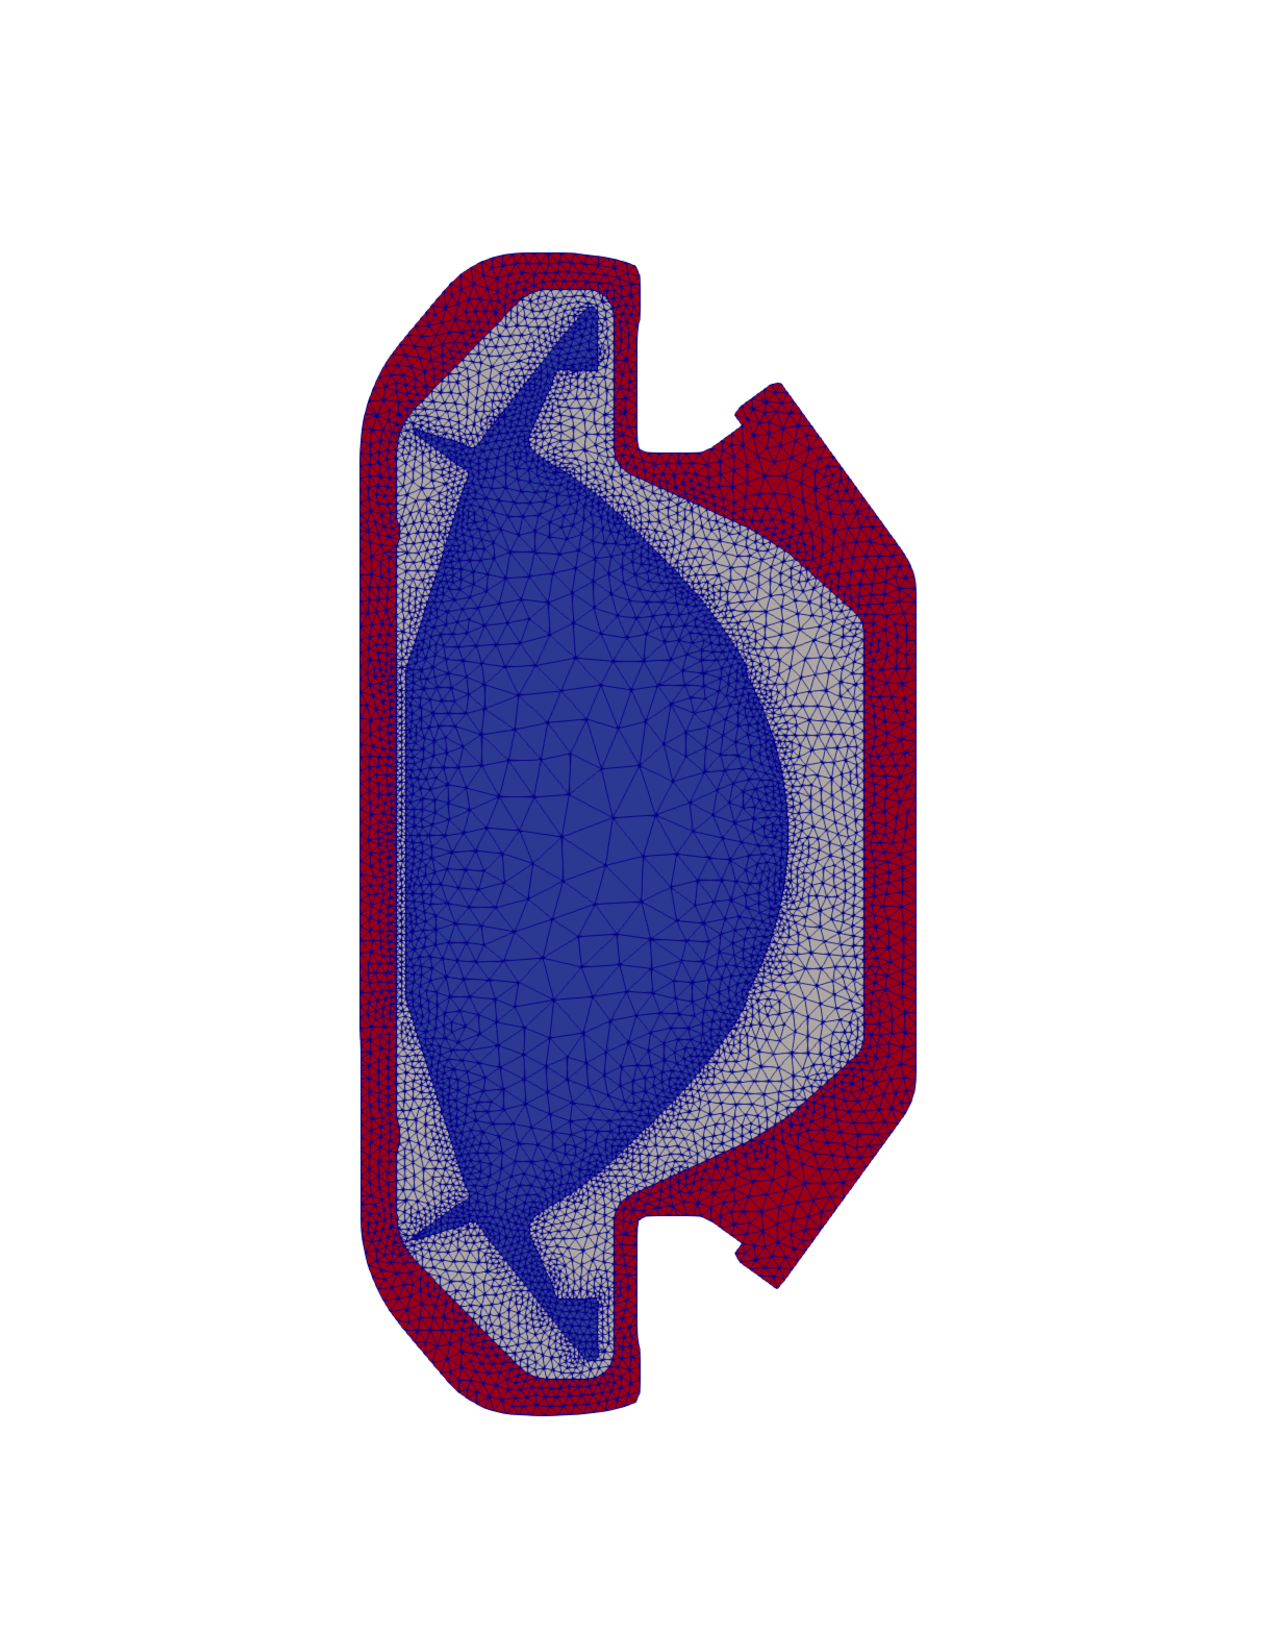
\includegraphics[width=3in]{./figures/meshgen-input3-novacuum.pdf}
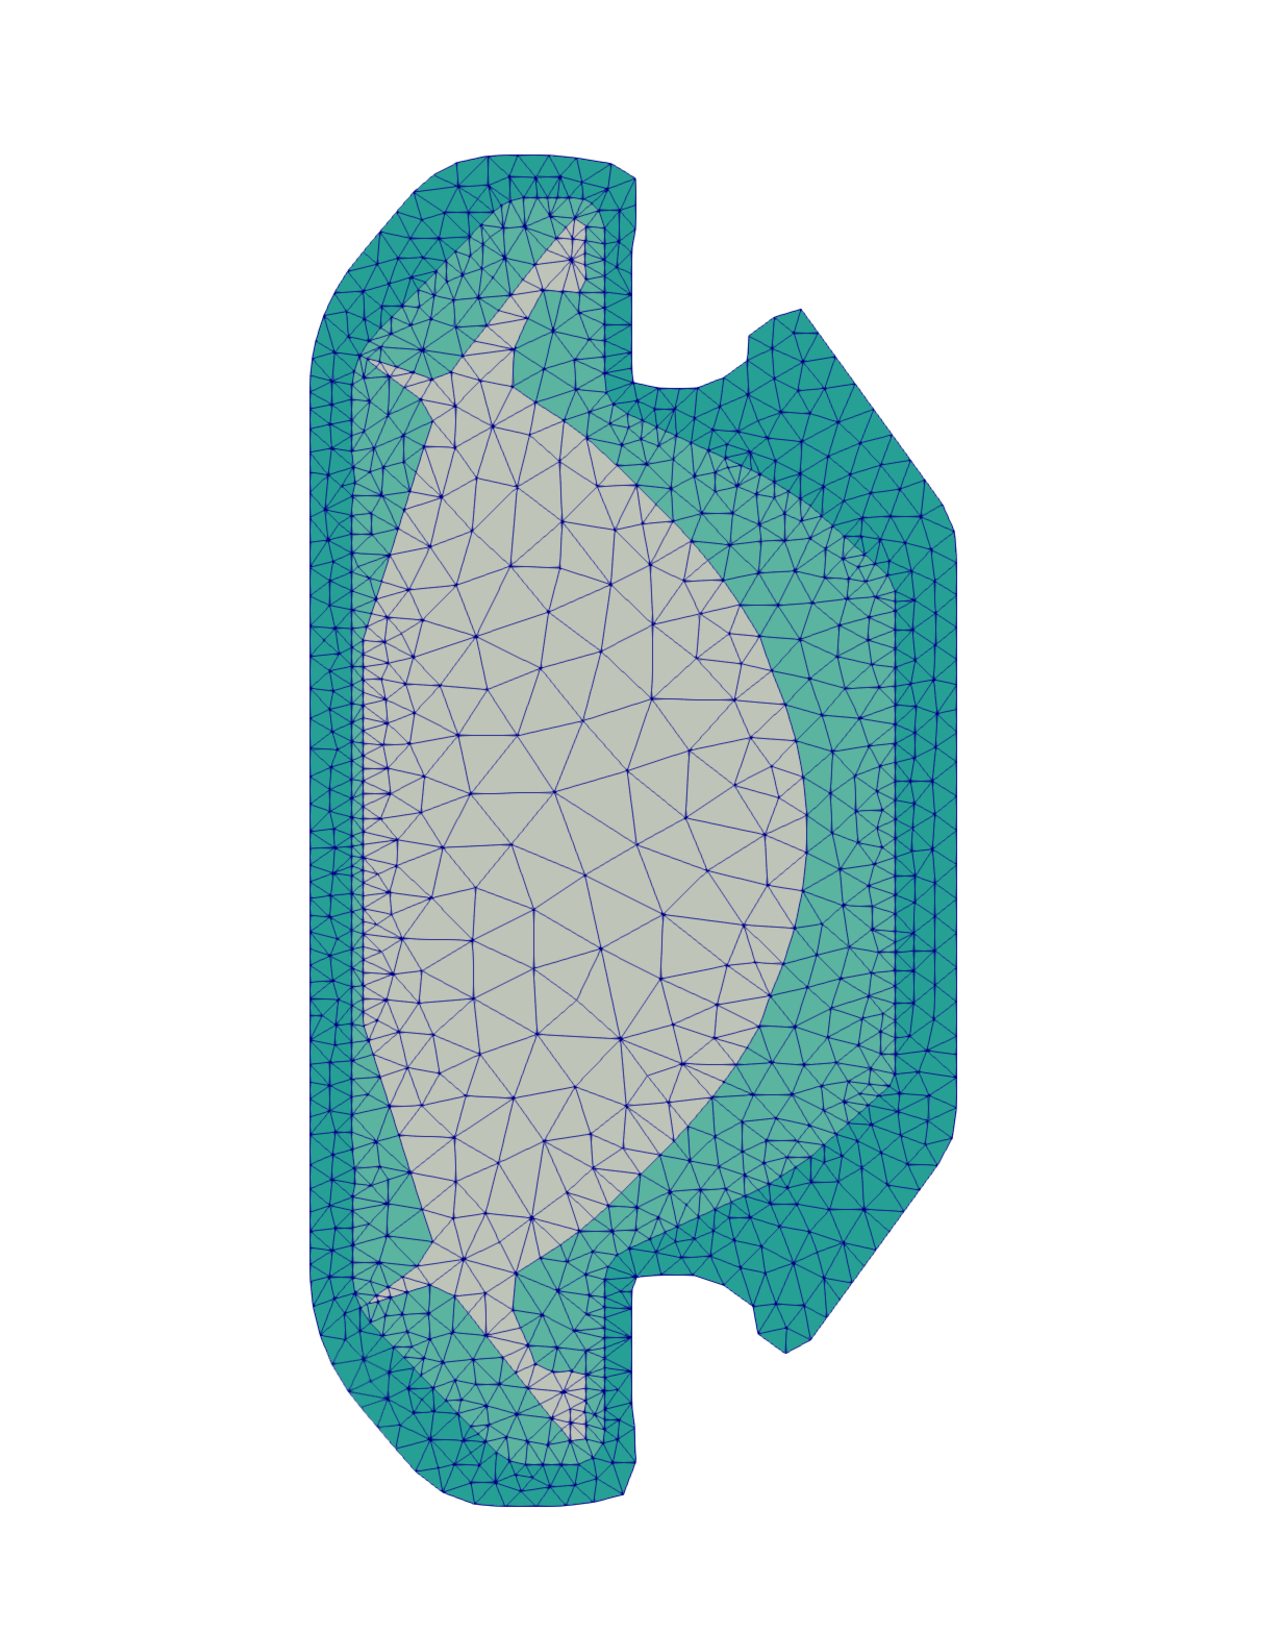
\includegraphics[width=3in]{./figures/meshgen-input3-novacuum2.pdf}
\caption
{Mesh with three boundary files and different meshGradationRate (left) 0.3 (right) 0.9}
\label{fig:input3-novacuum}
\end{figure}

\begin{verbatim}
numBdry 3
bdryFile loop1.dat 3 0.1
bdryFile loop2.dat 10 0.05
bdryFile loop3.dat 11 0.09

numFace 3
faceBdry  1 3 0.2
faceBdry  2 3 10 0.1
faceBdry  2 10 11 0.09

outFile input3
\end{verbatim}

The figure~\ref{fig:input3-novacuum} presents the mesh generated by the input file above.

%%%%%%%%%%%%%%%%%%%%%%%%%%%%%%%%%%%%%%%%%
\subsubsection{Mesh with seven boundary files and a vacuum wall}
%%%%%%%%%%%%%%%%%%%%%%%%%%%%%%%%%%%%%%%%%

\begin{figure}
\centering
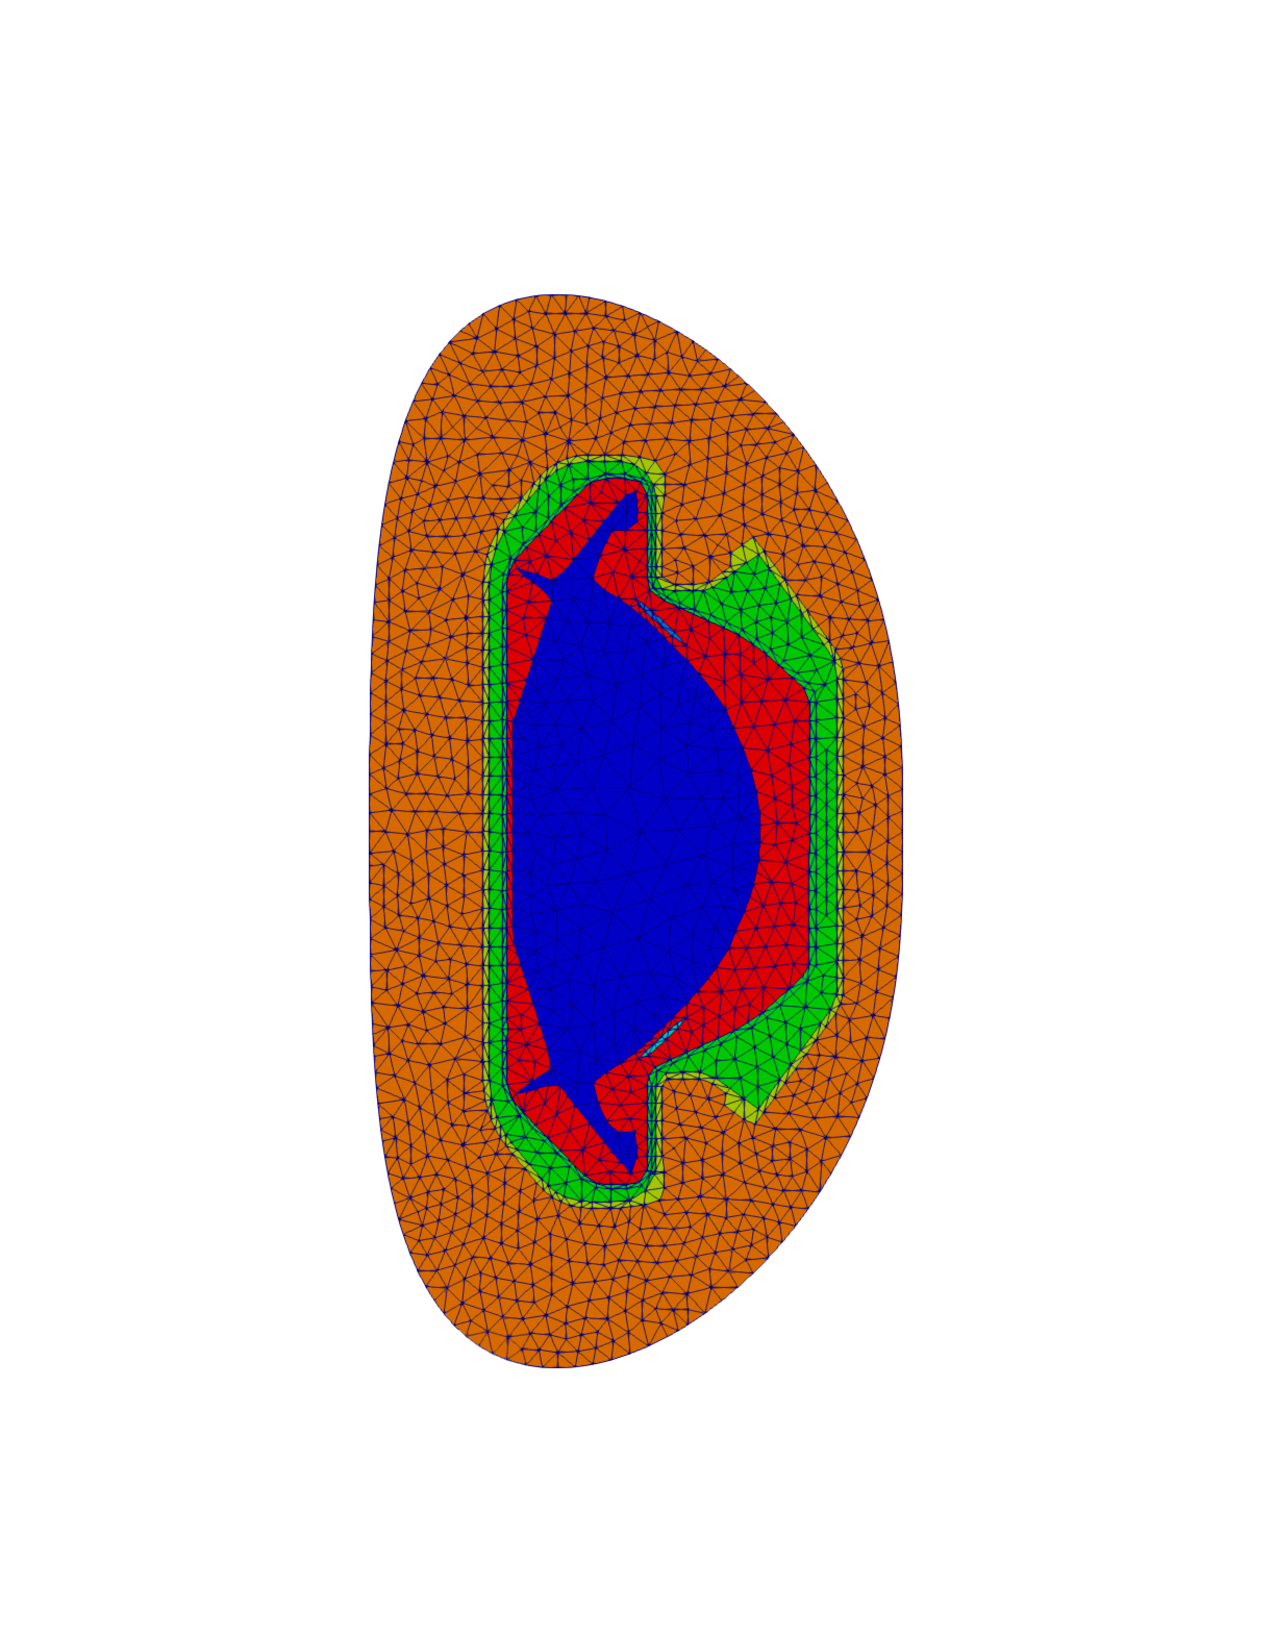
\includegraphics[width=4in]{./figures/meshgen-input7.pdf}
\caption{Mesh with seven boundary files and a parameterized vacuum wall}
\label{fig:input7-vacuum}
\end{figure}

\begin{verbatim}
numBdry 7
bdryFile loop1.dat 3 0.2
bdryFile loop2.dat 10 0.3
bdryFile loop3.dat 11 0.4
bdryFile loop4.dat 21 0.4
bdryFile loop5.dat 25 0.4
bdryFile loop6.dat 17 0.2
bdryFile loop7.dat 19 0.1

useVacuum 1 9 0.1
vacuumParams 1.8 1.5 0.4 0.0 2.5

numFace 8
faceBdry  1 3 0.2
faceBdry  1 10 0.3
faceBdry  1 11 0.1
faceBdry  2 21 25 0.2
faceBdry  2 25 17 0.09
faceBdry  2 17 19 0.1
faceBdry  2 19 9 0.1
faceBdry  4 3 10 11 21 0.11

outFile input7
\end{verbatim}

The figure~\ref{fig:input7-vacuum} presents the mesh generated by the input file above.

%%%%%%%%%%%%%%%%%%%%%%%%%%%%%%%%%%%%%%%%%
\subsubsection{Mesh with finite thickness wall and layers}
%%%%%%%%%%%%%%%%%%%%%%%%%%%%%%%%%%%%%%%%%

\begin{figure}
\centering
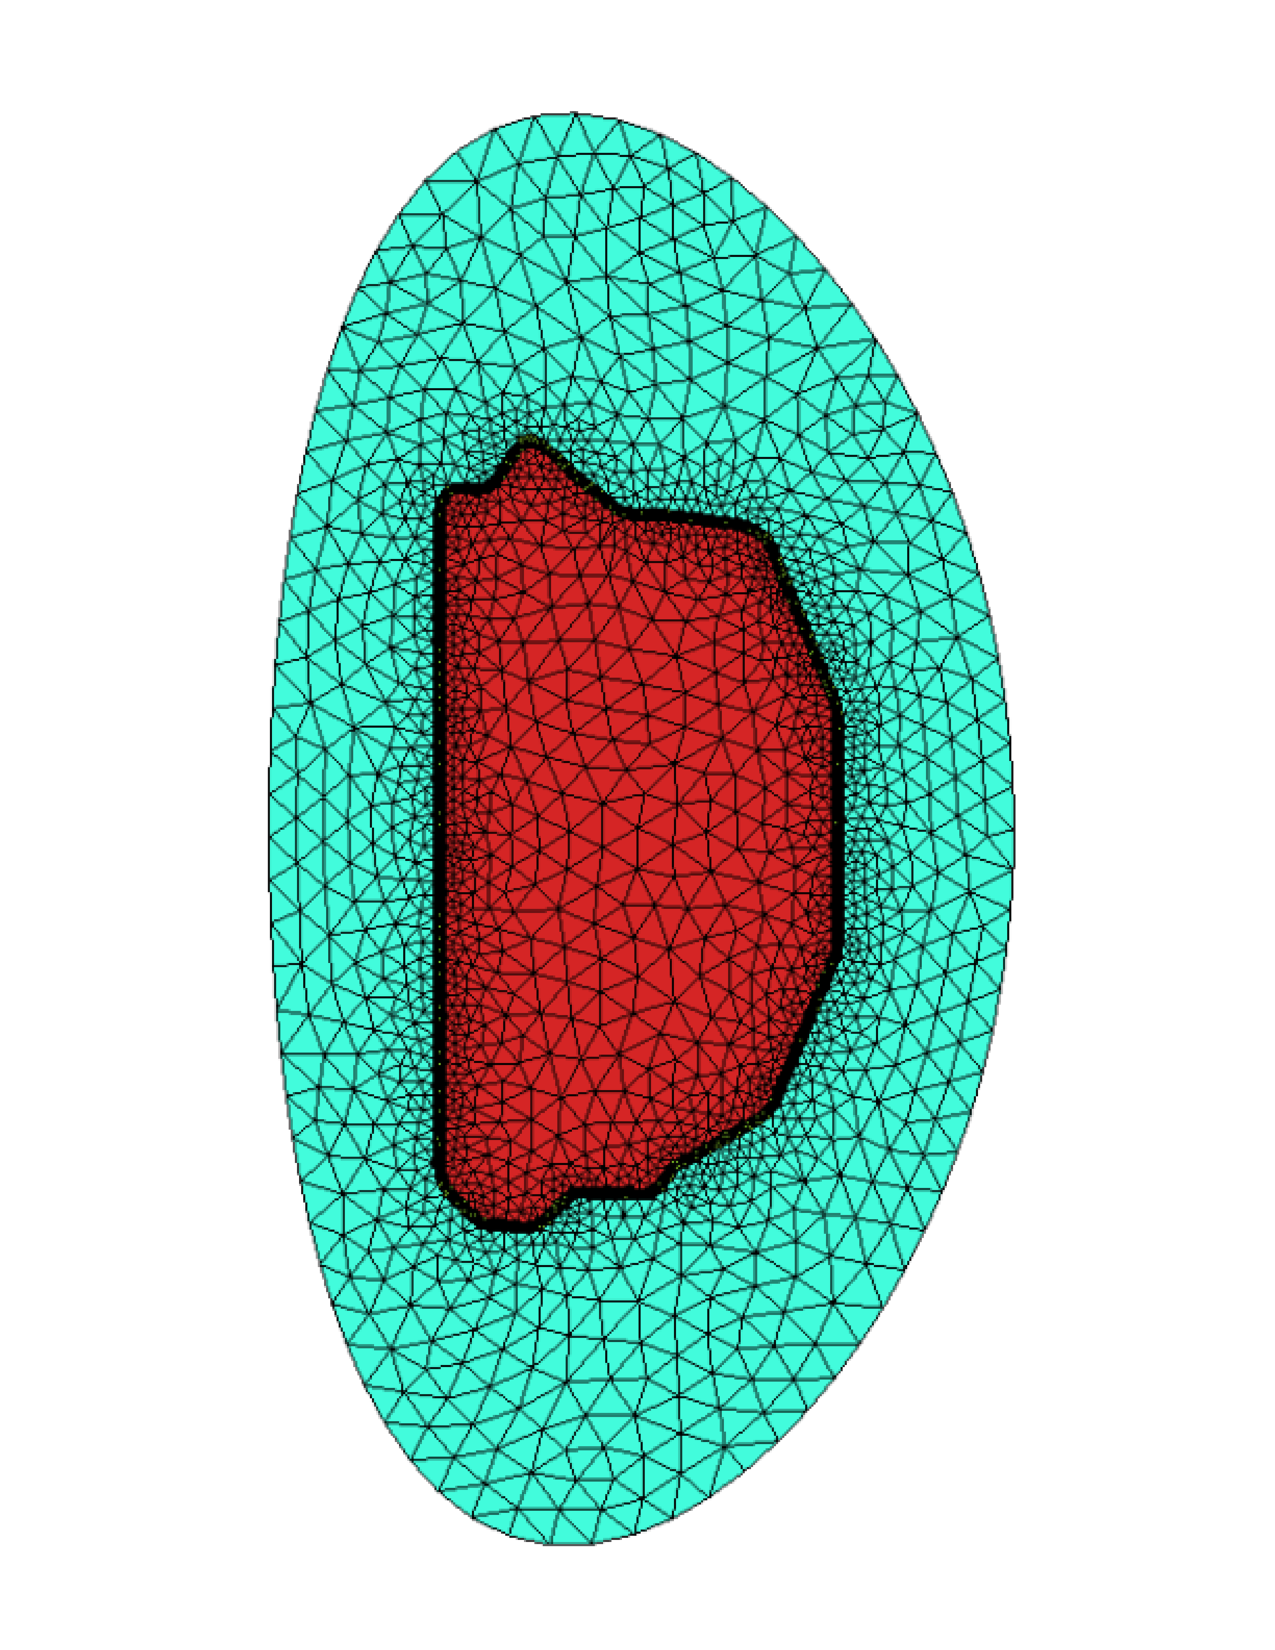
\includegraphics[width=3.5in]{./figures/FiniteThicknessWall-full.pdf}
\caption
{Add Caption Here}
\label{fig:thickness-full}
\end{figure}

\begin{figure}
\centering
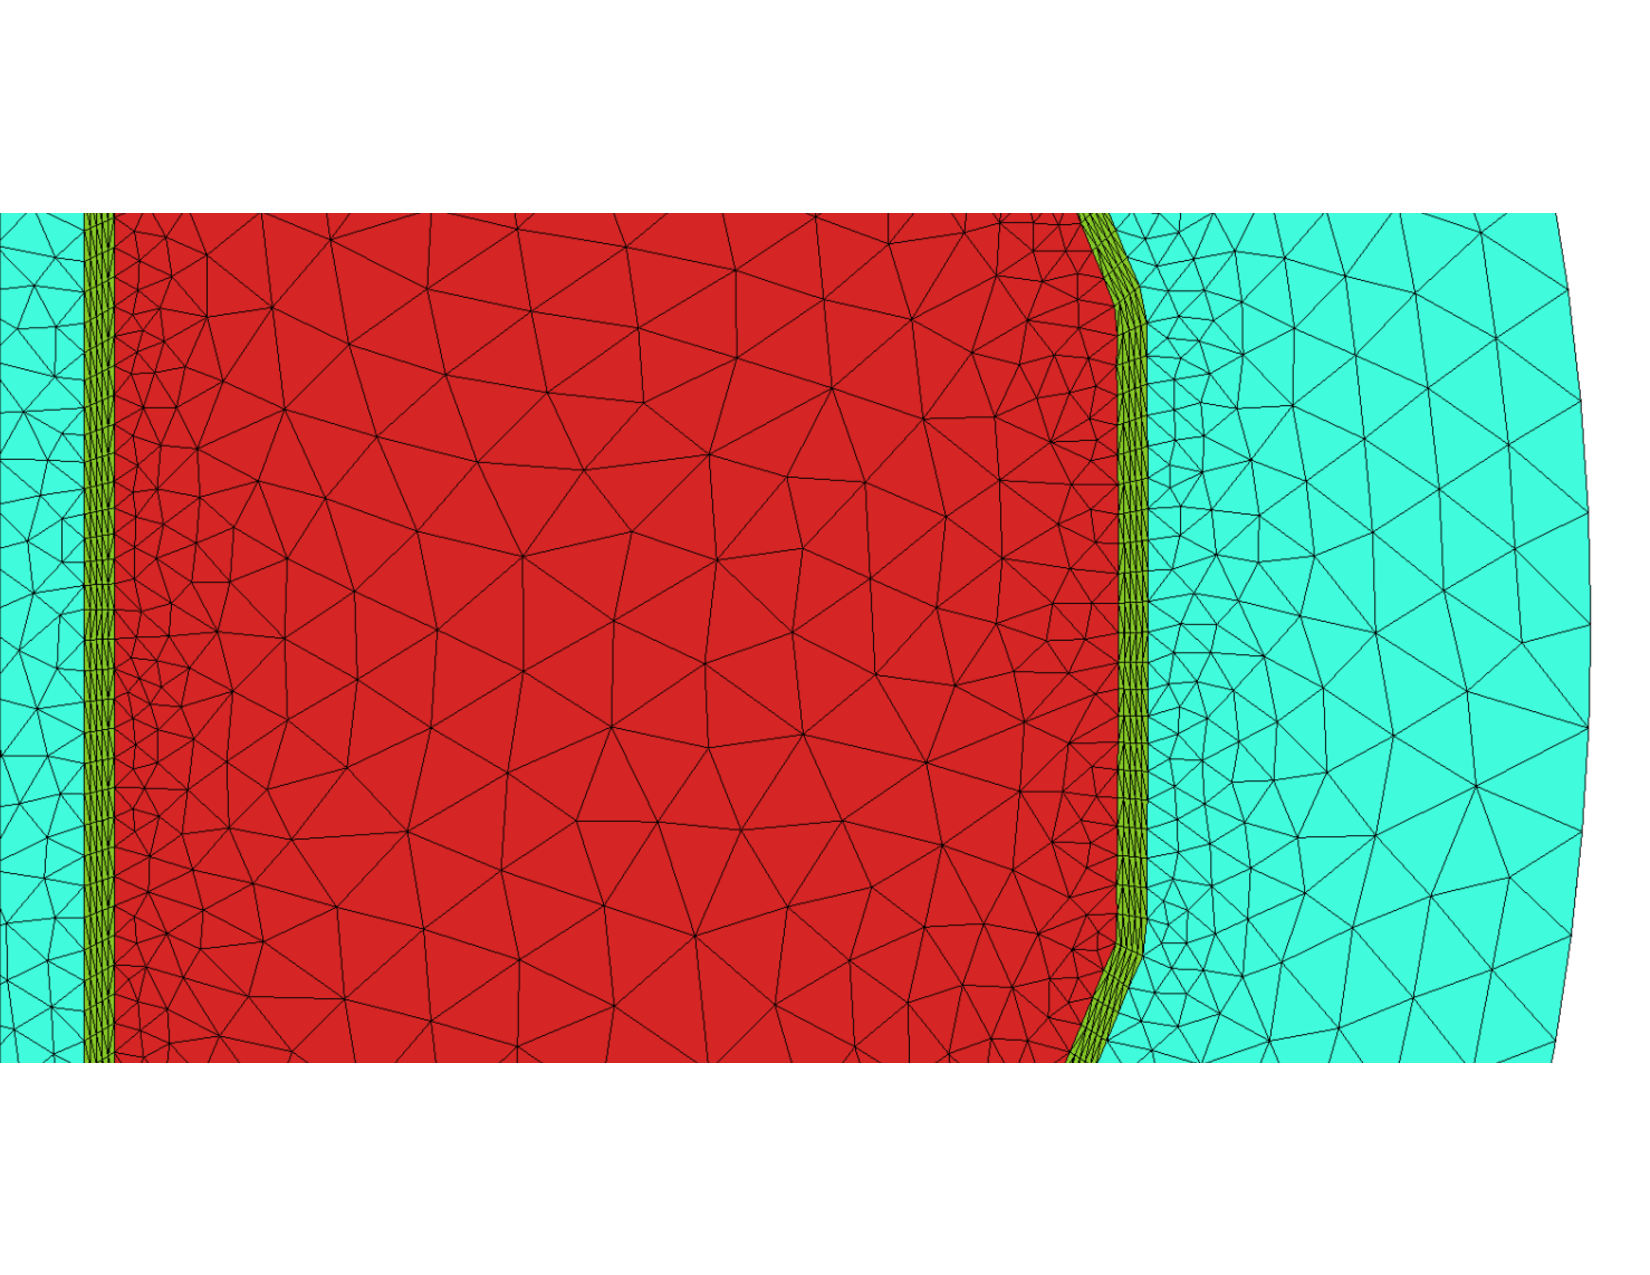
\includegraphics[width=2.5in]{./figures/FiniteThicknessWall-zoom1.pdf}
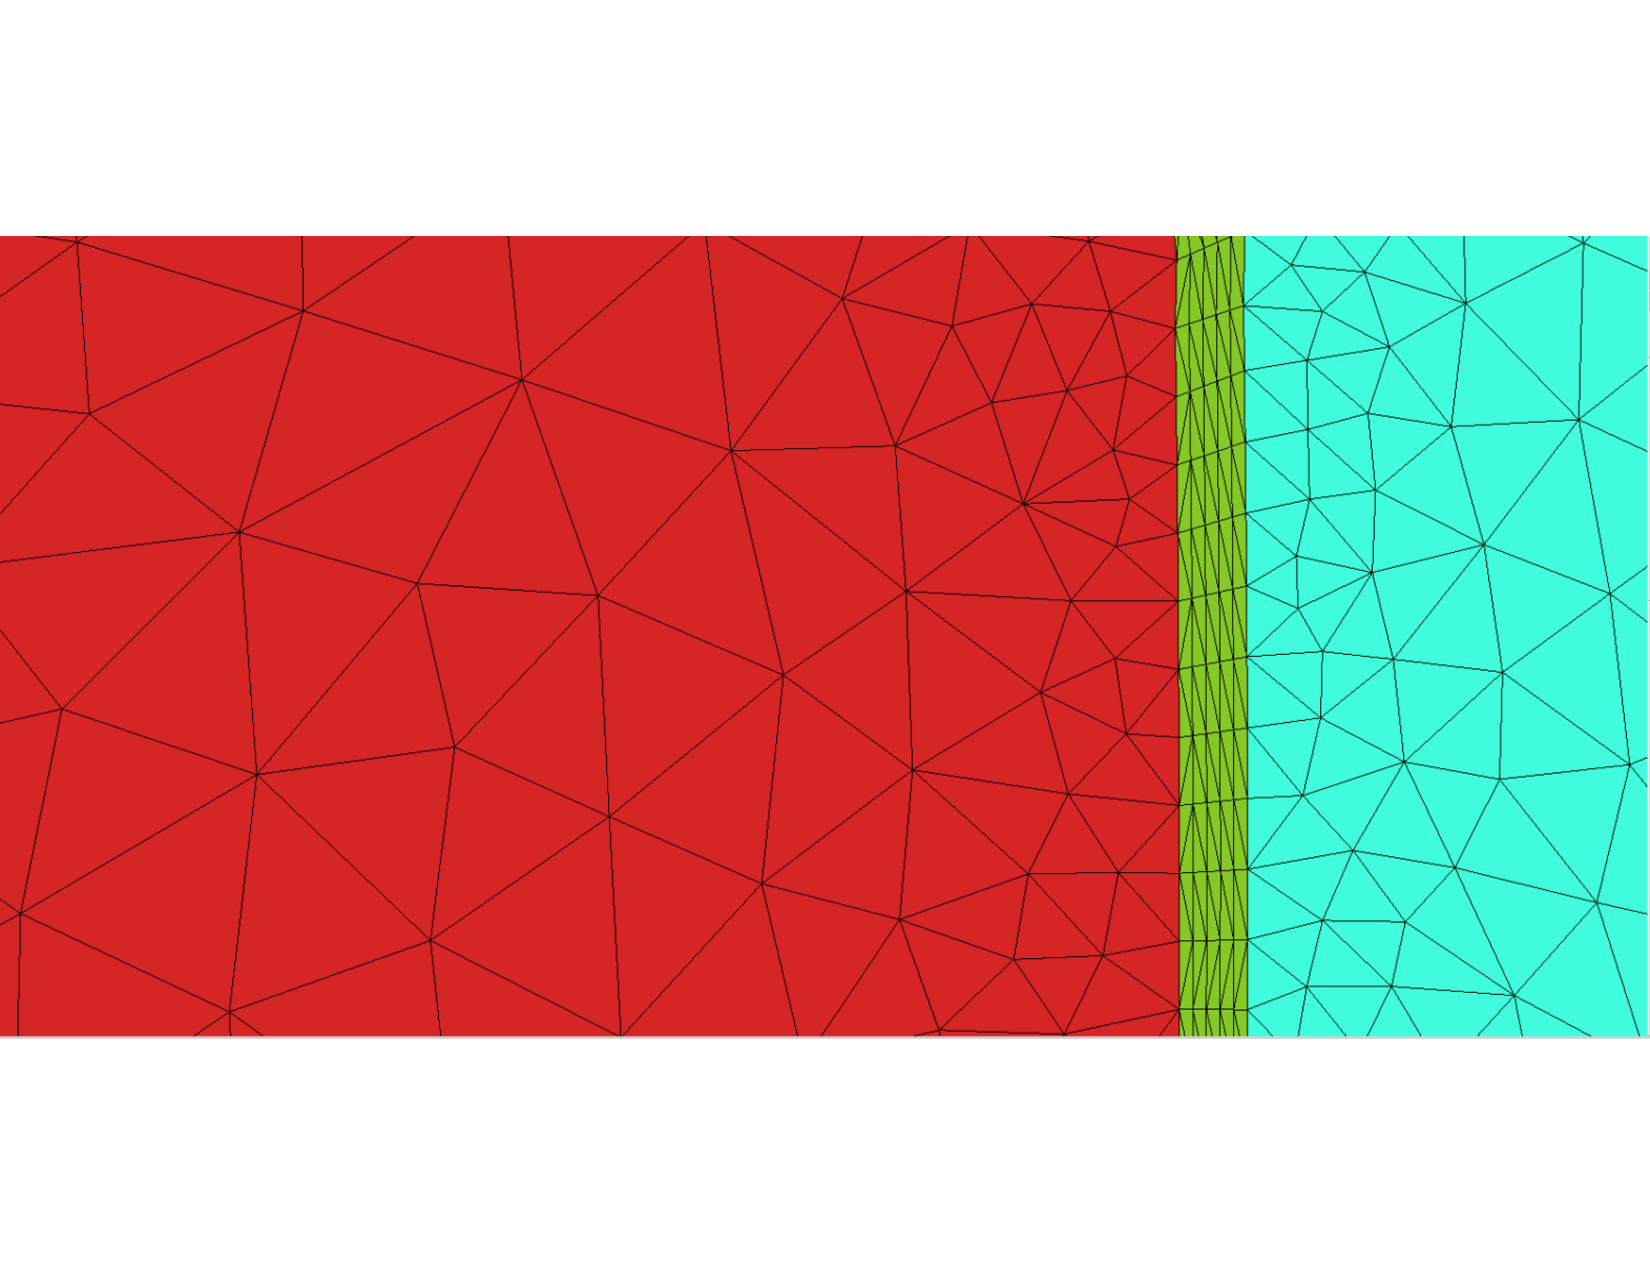
\includegraphics[width=2.5in]{./figures/FiniteThicknessWall-zoom2.pdf}
\caption
{Add Caption Here}
\label{fig:thickness-zoom}
\end{figure}

Add text here

%%%%%%%%%%%%%%%%%%%%%%%%%%%%%%%%%%%%%%%%%
\subsection{polar\_meshgen}
\label{ch:polar-gen}
%%%%%%%%%%%%%%%%%%%%%%%%%%%%%%%%%%%%%%%%%
\texttt{polar\_meshgen} requires an ascii file of arbitrary name that contains input parameters as the following:
\begin{itemize}
\item inFile: input file name containing equilibrium generation by jsolver
\item outFile: output file name to save model and mesh
\item meshSize: relative mesh size for each region (default 0.05)
\item reorder: if 1, reorder PUMI mesh based on adjacency (default: 0) and generate vtk folders for mesh visualization. The mesh before and after reodering is saved in \texttt{original-mesh.vtk} and \texttt{reordered-mesh.vtk}, respectively. Note that the element order of Simmetrix mesh is not affected.
\end{itemize}

The following presents an example input file ``\texttt{polar\_input}''.
\begin{verbatim}
inFile POLAR
outFile polar
meshSize 0.04
\end{verbatim}

To run \texttt{polar\_meshgen}, place \texttt{polar\_input} and \texttt{POLAR} in your work folder and do ``\texttt{polar\_meshgen polar\_input}''. The program will read \texttt{POLAR} and generate various model and mesh files starting with ``polar''. For instance, \texttt{polar-2K0.smb, pol-2K.sms, pol-2K.vtk, polar.dmg, polar.smd, polar.txt}. If the resulting mesh is too fine, increase the value of \texttt{meshSize}. If the resulting mesh is too coarse, decrease the value of \texttt{meshSize}. If \texttt{meshSize} is not specified in the input file, the default value is 0.05.   

The program \texttt{read\_jsolver} generates equilibrium and stores in the file \texttt{POLAR}. Given the input file \texttt{POLAR}, \texttt{m3dc1\_meshgen} generates the following files:
\begin{itemize}
\item	model.dmg: PUMI-readable model file
\item	model.txt: M3DC1-readable model file
\item	mesh0.smb: PUMI/M3DC1-readable mesh file
\item	mesh.vtk: Paraview data files
\item	norm\_curv: ascii file containing nodes' normal/curvature information
\end{itemize} 

%%%%%%%%%%%%%%%%%%%%%%%%%%%%%%%%%%%%%%%%%
\subsection{Mesh Control with SimModeler}
SimModeler is a graphical user interface to the Simmetrix geometry and mesh generation software. In cases where the currently available capabilities of m3dc1\_meshgen do not provide a satisfactory mesh, SimModeler can be used to apply alternative mesh control information to the Tokamak cross section geometry to generate different meshes. The information below indicates the application of a subset of the mesh controls that can be applied. For additional information of the full range of SimModeler mesh control options see: ********** FILL IN POINTER TO SIMMETRIX DOCUMENTATION *****
\label{ch:simmodeler}
%%%%%%%%%%%%%%%%%%%%%%%%%%%%%%%%%%%%%%%%%
(Contributed by D. Pfefferle on 4/27/16) On PPPL Portal, load a module \texttt{simmodeler} and run it.
\begin{enumerate}
\item From the menu \texttt{"File$\rightarrow$Open Model"}, load a model file (\texttt{.smd}) generated by \texttt{m3dc1\_meshgen}
\item In the upper panel, in the views section, click on \texttt{Front} to view the model, then go to \texttt{Meshing} tab
\item Select outer region, click \texttt{+} in \texttt{Mesh Attributes} and select \texttt{Mesh Size$\rightarrow$relative}. 
Enter a value (typically 0.1)
\item Select wall region, click \texttt{+} in \texttt{Mesh Attributes} and select \texttt{Mesh Size$\rightarrow$relative}. 
Enter a value (typically 0.02)
\item Select inner region, click \texttt{+} in \texttt{Mesh Attributes} and select \texttt{Mesh Size$\rightarrow$relative}. 
Enter a value (typically 0.04). Here, one can already generate the mesh by clicking on \texttt{Generate Mesh} and verify if the mesh sizes are suitable 
\item 	Select both inner and wall regions (holding shift key), click \texttt{+} in \texttt{Mesh Attributes} and select \texttt{Mesh Size$\rightarrow$relative}. Enter a function, e.g. \texttt{0.01$\times$abs(\$y+1.5)\^{}2+0.004} to specify an anisotropic mesh density on top of previous settings
\\ There are many available parameters for fine-tuning the mesh density.  For example, \texttt{Mesh Curvature Refinement} with parameter packs more elements near the edges of the resistive wall. 
\item \texttt{Generate Mesh} and \texttt{Show Mesh} to view result in new windows
\item If the result is satisfactory, from the menu \texttt{File$\rightarrow$Save Mesh}, give it a meaningful name with the extension \texttt{.sms}. The original model file \texttt{.smd} has been automatically saved by the program with your mesh modifications.
\item Close \texttt{simmodeler} then it will release a license. Until you quit Simmodeler, no one cannot run neither \texttt{m3dc1\_meshgen} nor \texttt{simmodeler}.
\item Copy the \texttt{.txt, .smd} and \texttt{.sms} files to the simulation directory and run the following splitting routine to obtain PUMI-readable \texttt{.smb} mesh files.
\newline\newline
\texttt{/p/tsc/C1/m3dc1-sunfire.r6-1.5/bin/part\_mesh.sh model\_file.smd mesh\_file.sms X}, 
where \texttt{X} is the number of parts you need in the \texttt{.smb} mesh.
\item Modify the \texttt{C1input} file accordingly
\newline\newline
\texttt{mesh\_filename = `part.smb'
\\
mesh\_model = `filename.txt'
}
\end{enumerate}

%%%%%%%%%%%%%%%%%%%%%%%%%%%%%%%%%%%%%%%%%
\subsection{Mesh Partitioning}
\label{ch:mesh-ptn}
%%%%%%%%%%%%%%%%%%%%%%%%%%%%%%%%%%%%%%%%%

\subsubsection{Splitting}

The program \texttt{split\_smb} increases the number of parts in a mesh from \texttt{P} to \texttt{N} (\texttt{P$<$N}). 
In each machine, the program \texttt{split\_smb} is availble in \texttt{\$SCOREC\_UTIL\_DIR} provided in \texttt{hostname.mk} file.

In order to split \texttt{P}-part mesh to \texttt{N} parts (\texttt{N$>$P}), run
\texttt{"mpirun -np N ./split\_smb input-mesh(.smb) output-mesh(.smb) X"}
\begin{itemize}
\item	the file extension of input-mesh should be .smb 
\item	the file extension of output-mesh should be .smb
\item	\texttt{N} is the number of parts in the output mesh
\item	For a \texttt{P}-part input mesh, \texttt{X} must be \texttt{N/P}
\item	For both input and output mesh, do not specify a number before the file extension
\item	\texttt{split\_smb} will insert a number in the output mesh file. The number represents a global part ID.
\item	Make sure that the output mesh doesn't have any empty part. Otherwise, the program crashes with the following error message:
\newline
\texttt{APF warning: 1 empty parts}
\newline
\texttt{split\_smb: \ldots/mds/mds.c:614: check\_ent: Assertion `e $>$= 0' failed}
\end{itemize}

Examples on portal:
\begin{enumerate}
\item To split a serial (1-part) mesh to 6 parts, run\\
 \texttt{"mpirun -np 6 ./split\_smb struct-curveDomain.smb part.smb 6"}
\begin{itemize}
\item	Input mesh: struct-curveDomain0.smb 
\item	Output mesh: part0.smb, part1.smb, part2.smb, part3.smb, part4.smb, part5.smb
\end{itemize}

\item To split a 2-part mesh to 6 parts, run
 \texttt{"mpirun -np 6 ./split\_smb  struct-curveDomain.smb part.smb 3"}
\begin{itemize}
\item	Input mesh: struct-curveDomain0.smb, struct-curveDomain1.smb
\item	Output mesh: part0.smb, part1.smb, part2.smb, part3.smb, part4.smb, part5.smb
\end{itemize}
\end{enumerate}

See \texttt{readme.split\_smb} for detailed instructions and trouble shooting tips.

%%%%%%%%%%%%%%%%%%%%%%%%%%%%%%%%%%%%%%%%%
\subsubsection{Mesh Merging}
\label{ch:mesh-mg}
%%%%%%%%%%%%%%%%%%%%%%%%%%%%%%%%%%%%%%%%%

The program \texttt{collapse} decreases the number of parts in a mesh from \texttt{N} to \texttt{P} (\texttt{P$<$N}). 
In each machine, the program \texttt{collapse} is availble in \texttt{\$SCOREC\_UTIL\_DIR} provided in \texttt{hostname.mk} file.

In order to merge \texttt{N}-part .smb mesh to \texttt{P} parts (\texttt{P$>$0}), run
\texttt{"mpirun -np N ./collapse input-mesh(.smb) output-mesh(.smb) X"}
\begin{itemize}
\item	the file extension of input-mesh should be .smb 
\item	the file extension of output-mesh should be .smb
\item	\texttt{N} is the number of parts in the input mesh
\item	For a \texttt{P}-part output mesh, \texttt{X} must be \texttt{N/P}
\item	For both input and output mesh, do not specify a number before the file extension
\item	\texttt{collapse} will insert a number in the output mesh file. The number represents a global part ID.
\end{itemize}

Example on portal:
\newline
In order to merge 4-part mesh into a serial (1-part) mesh, run
\texttt{"mpirun -np 4 ./collapse part.smb serial.smb 4"}
\begin{itemize}
\item	Input mesh: part0.smb, part1.smb, part2.smb, part3.smb
\item	Output mesh: serial0.smb
\end{itemize}

See \texttt{readme.collapse} for detailed instructions and trouble shooting tips.

%%%%%%%%%%%%%%%%%%%%%%%%%%%%%%%%%%%%%%%%%
\subsection{Miscellaneous}
\label{ch:mesh-misc}
%%%%%%%%%%%%%%%%%%%%%%%%%%%%%%%%%%%%%%%%%

\subsubsection{Verification}

The program \texttt{check\_smb} investigates an input mesh and prints any invalid aspects of the mesh. At the end, the mesh size (the number of global, local, and owned entities per dimension) is printed. 

In order to run, do \texttt{"mpirun -np N ./check\_smb input-mesh(.smb)"}.


\section{Mesh Adaptation by Error Estimator}


\include{numerical-methods}

\section{Output}

\subsection{HDF5 Output}

By default, M3D-C1 will output data to a HDF5 file named \texttt{C1.h5}.  The file is organized as follows:

\begin{itemize}
\item state variables
\item \texttt{scalars/}
\item \texttt{equilibrium/}
\item \texttt{time\_\#\#\#/}
\end{itemize}  

\subsubsection{State variables}

\subsubsection{The \texttt{scalars/} group}

The \texttt{scalars/} group contains one-dimensional time series data,
output at every MHD timestep.  Some of the time series that are output
include the following:

\begin{tabular}{lll}
\textbf{Scalar}   & \textbf{Units} & \textbf{Description} \\
\hline
time              & $t_0$          & The physical time at each MHD timestep\\
dt                & $t_0$          & The physical time per MHD timestep\\ 
loop\_voltage     & $V_0$          & The loop voltage applied at the domain boundary\\
toroidal\_current & $I_0$          & The total toroidal current in the MHD region\\
particle\_number  & $n_0 L_0^3$    & The total number of main ions in the MHD region\\
electron\_number  & $n_0 L_0^3$    & The total number of electrons in the MHD region\\
power\_injected   & $p_0 L_0^3 / t_0$ & The total power from the heat source in the MHD region
\end{tabular}

For simulations that make use of the KPRAD module, the following time
series are also output:

\begin{tabular}{lll}
\textbf{Scalar}   & \textbf{Units} & \textbf{Description} \\
\hline
radiation & $p_0 L_0^3 / t_0$ & Total power loss due to all radiation sources\\
line\_rad & $p_0 L_0^3 / t_0$ & Power loss due to line radiation\\
brem\_rad & $p_0 L_0^3 / t_0$ & Power loss due to bremsstrahlung\\
ion\_loss & $p_0 L_0^3 / t_0$ & Power loss due to ionization\\
reck\_rad & $p_0 L_0^3 / t_0$ & \\
recp\_rad & $p_0 L_0^3 / t_0$ & \\
kprad\_n  & $n_0 L_0^3$ & Total number of impurity nuclei (both ionized and neutral)\\
kprad\_n0 & $n_0 L_0^3$ & Total number of neutral impurity atoms\\
kprad\_dt & $t_0$       & Time step of KPRAD subcycle
\end{tabular}


\subsubsection{The \texttt{equilibrium/} and \texttt{time\_\#\#\#/} groups}

The \texttt{equilibrium/} and \texttt{time\_\#\#\#/} groups contain the
mesh and field data upon initialization (\texttt{equilibrium/} and
\texttt{time\_000/}) and at each field output time slice
(\texttt{time\_\#\#\#}).  The number of MHD timesteps per field output
time slice is determined by the C1input parameter \texttt{ntimepr}.

In calculations with eqsubtract=1, the \texttt{equilibrium/} group
contains the equilibrium part of the fields whereas \texttt{time\_\#\#\#/}
contain the perturbed part of the fields.

The data in \texttt{equilibrium/} and \texttt{time\_\#\#\#} are written to
separate files named \texttt{equilibrium.h5} and
\texttt{time\_\#\#\#.h5}.  These files are linked to \texttt{C1.h5} using
the linking feature of HDF5 so that the data can be accessed as if it
were a regular group in \texttt{C1.h5}.

\begin{tabular}{lll}
\textbf{Variable} & \textbf{Units} & \textbf{Description}\\
\hline
time              & $t_0$ & Physical time of time slice\\
nspace            & 1     & 2 for 2D / complex; 3 for 3D simulations\\
ntimestep         & 1     & MHD timestep associated with this times lice\\
version           & 1     & Version number for output data\\
mesh/             &       & Mesh data group\\
mesh/nelms        & 1     & Number of mesh elements\\
mesh/period       & 1     & Toroidal period of mesh\\
mesh/ifull\_torus & 1     & 1 if full-torus simulation; 0 if partial-torus simulation\\
mesh/nperiods     & 1     & If partial torus, number of periods per full torus\\
mesh/phi          & 1     & 1D array containing the toroidal angles of the toroidal planes\\
mesh/elements     &       & 2D array containing mesh data\\
mesh/adjacency    &       & 2D array containing adjacency data\\
fields/           &       & Group containing field data
\end{tabular}

\begin{figure}
\begin{center}
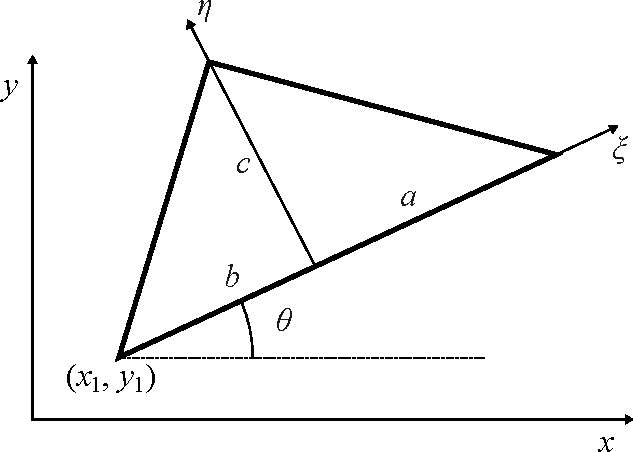
\includegraphics{figures/C1_element.pdf}
\caption{\label{fig:C1}The geometry of a mesh element in the toroidal plane\cite{Jardin04}}
\end{center}
\end{figure}

\paragraph{\texttt{mesh/elements}} is a 2D array consisting of
\texttt{nelms} rows (one per mesh element), with 8 (for 2D
simulations) or 10 (for 3D simulations) columns:

\[ a, b, c, \theta, x_1, y_1, \text{ibound}, \text{izone}, d, \varphi_1 \]

The first five columns ($a$ through $y_1$) describe the geometry of
the element in the toroidal plane, as illustrated in
figure~\ref{fig:C1}.  $d$ and $\varphi_1$ represent the toroidal
extent of the element and the toroidal coordinate of the first
bounding plane (in radians if itor=1, in units of $L_0$ otherwise),
and are only present for 3D simulations.

\paragraph{Fields/} is a group containing the field data.  Each field
is a 2D array consisting of \texttt{nelms} rows (one per element) and
20 (in 2D) or 80 (in 3D) columns, representing the coefficients of
each shape function within the given mesh element.

The field $\phi$ at the coordinate system $(\xi,\eta,\zeta)$ local to the mesh element is given by
\[ 
  \phi(\xi,\eta,\zeta) = \sum_{j=0}^{J} \sum_{i=1}^{20} a_{i + 4(j-1)} \xi^{m_i} \eta^{n_i} \zeta^j
\]
where
\begin{eqnarray*}
   m & = & \{0,1,0,2,1,0,3,2,1,0,4,3,2,1,0,5,3,2,1,0 \}\\
   n & = & \{0,0,1,0,1,2,0,1,2,3,0,1,2,3,4,0,2,3,4,5 \}\\
\end{eqnarray*}
and where $J=3$ for 3D simulations and $J=0$ for 2D / complex simulations.

The fields that are written include the following.  (Note that in 2D
complex simulations, these field names contain the real part of the
field data; for each field an additional field with the suffix "\_i"
is written to contain the imaginary part.)

\begin{tabular}{llll}
\textbf{Field} & \textbf{Units (itor=1)} & \textbf{Units (itor=0)} & \textbf{Description}\\
\hline
psi  & $B_0 L_0^2$ & $B_0 L_0$   & $\psi$\\
I    & $B_0 L_0$   & $B_0$       & $F$ \\
f    & $B_0 L_0$   & $B_0 L_0^2$ & $f$ \\
phi  & $v_0$       & $v_0 L_0$   & $U$ \\
V    & $v_0/L_0$   & $v_0$       & $\omega$ \\
chi  & $v_0 L_0^3$ & $v_0 L_0$   & $\chi$ \\
P    & $p_0$       & $p_0$       & $p$ \\
Pe   & $p_0$       & $p_0$       & $p_e$ \\
ti   & $T_0$       & $T_0$       & $T_i$ \\
te   & $T_0$       & $T_0$       & $T_e$ \\
den  & $n_0$       & $n_0$       & $n_i$ \\
ne   & $n_0$       & $n_0$       & $n_e$
\end{tabular}



\section{PETSc Option}
\label{petscoption}

\subsection{2D}

\noindent
The petsc option to run 2D modes is default to superlu\_dist. You can add the following line on your "srun" command line
to change to to mumps:

\begin{verbatim}
-pc_factor_mat_solver_type mumps
\end{verbatim}

\subsection{3D}

\noindent
When running M3D-$C^1$ in the 3D nonlinear mode, you need to include PETSc Options file.
There is a number "8" in the file below. It must be equal to the number of toroidal planes. It
should be changed whenever you change the number of toroidal planes in the C1input file. The recommended
{\it options\_bjacobi} file is as follows:

\begin{verbatim}
-pc_type bjacobi
-pc_bjacobi_blocks 8
    (for 8 toroidal planes should be equal to nplanes in C1input)
-sub_pc_type lu
-sub_pc_factor_mat_solver_package superlu_dist
    (can exchange mumps for superlu_dist)
-mat_superlu_dist_rowperm NOROWPERM (only needed for superlu_dist)
-mat_mumps_icntl_14 50 (only needed for mumps)
    (50 means 50% of memory increase when needed.
     Users can make it 100 or more if encountering a runtime memory issue.)
-sub_ksp_type preonly
-ksp_type fgmres
-ksp_gmres_restart 220
-ksp_rtol 1.e-9
-ksp_max_it 10000
-on_error_abort

-hard_pc_type bjacobi
-hard_pc_bjacobi_blocks 8
    (for 8 toroidal planes…should be equal to nplanes in C1input)
-hard_sub_pc_type lu
-hard_sub_pc_factor_mat_solver_type superlu_dist
    (can change mumps for superlu_dist)
-mat_superlu_dist_rowperm NOROWPERM
    (only needed for superlu_dist)
-mat_mumps_icntl_14 50
    (only needed for mumps.)
    (50 means 50% of memory increase when needed.
     Users can make it 100 or more if encountering a runtime memory issue.)
-hard_sub_ksp_type preonly
-hard_ksp_type lgmres
-hard_ksp_lgmres_argument 4
-hard_ksp_gmres_restart 220
-hard_ksp_rtol 1.e-9
-hard_ksp_max_it 10000
\end{verbatim}

\subsection{More}

\noindent
More examples are in regtest/pellet/base/ directory, such as 

\begin{verbatim}
options_bjacobi.type_superludist
options_bjacobi.type_mumps 
\end{verbatim}

\noindent
The following are additional optional arguments:

\begin{verbatim}
-ksp_converged_reason
-ksp_view

-help

-options_table
-options_left

-trdump
-malloc_log
\end{verbatim}

for diagnosing purpose.


\section{Running Jobs}

\noindent
Users can find almost all of the needed example batch scripts and input files to run a job on available computing facilities from 
\begin{verbatim}
unstructured/regtest/*/base/
\end{verbatim}

\noindent
directories.

\subsection{Running 2D or Linear Jobs}

\noindent
In 2D, the run can be either linear or nonlinear, depending on the C1input parameter $linear$:

$linear=0$ (non-linear run: must compile with the option RL=1)

$linear=1$ (linear run: must compile with the option COM=1)

\noindent
In both cases, set 

$nplanes=1$

For the linear case, use

$ntor=nn$

set the toroidal mode number.

\noindent
To run your job on a scratch directory, copy the following files over:
\begin{verbatim}
executable (m3dc1_2d for non-linear run or m3dc1_2d_complex for linear run)
C1input
AnalyticModel (or MultiEdgeAnalyticModel)
struct-dmg.sms
(and geqdsk if needed)
\end{verbatim}

To run non-linear job
\begin{verbatim}
mpirun –np 8 ./m3dc1_2d
\end{verbatim}

To run linear job
\begin{verbatim}
mpirun –np 24 ./m3dc1_2d_complex -pc_factor_mat_solver_package mumps 
\end{verbatim}

\subsection{Running 3D Nonlinear Jobs}

\noindent
For the 3D nonlinear run, set $linear=0$ and set $nplanes$ equal to the number of toroidal planes in $C1input$ file. The
number of bjacobi blocks in the PETSc options file must also be equal to $nplanes$. The
total number of processors to request must be the product of nplanes and M (the number of processors per plane, which equals the number of mesh partitions per plane).

\noindent
Files required to be present to the local directory are:
\begin{verbatim}
executable (m3dc1 or m3dc1_st)
C1input,
partnn.smb (one for each poloidal plane partition)
options_bjacobi
m3dc1.xml (if using ADIOS)
geqdsk (if needed)
\end{verbatim}

\noindent
To run linear job
\begin{verbatim}
mpirun –np 16 ./ m3dc1 –ipetsc –options_file options_bjacobi (nplane=2, M=8)
\end{verbatim}
\noindent
See the previou section for the format of the PETSc option file options\_bjacobi. In this example job, there are $M=8$ mesh partition files:
\begin{verbatim}
part0.smb part1.smb part2.smb part3.smb part4.smb part5.smb part6.smb part7.smb
\end{verbatim}

\subsection{Running Jobs with the Bootstrap Model}

\noindent
To run simulations with the bootstrap model enabled, the following procedure should be followed: 
\begin{enumerate}
    \item \textit{Initial Simulation Without Bootstrap Model}:  
    Run a simulation for a single timestep with the bootstrap model disabled. 

    \item \textit{Generate M3D-C1 output file}:  
    Using fusion-io, generate the \texttt{neo\_input.nc} file containing the density, temperature, magnetic field, and rotational transform outputs required to calculate the bootstrap coefficients ($L_{31}$, $L_{32}$, $L_{34}$, $\alpha$). These coefficients are necessary to run the bootstrap model.

    \item \textit{Generate Bootstrap Coefficients Input File}:  
    Execute the MATLAB script located in the fusion-io's \texttt{/util/matlab\_bootstrap} directory. Use the appropriate flags as specified in the script's README file.  
    This will generate a file named either:
    \begin{itemize}
        \item \texttt{ProfileJBSCoeff\_Te\_L31\_32\_34\_alpha\_B2\_dtedpsit\_G} or 
        \item \texttt{ProfileJBSCoeff\_Psi\_L31\_32\_34\_alpha\_B2\_dtedpsit\_G},
    \end{itemize}
    which will serve as input for the bootstrap model in M3D-C1.

    \item \textit{Rerun Simulation with Bootstrap Model Activated}:  
    Run the simulation again, this time using the file generated in the previous step and setting the appropriate model options. The following settings are recommended for the \texttt{C1input} file to activate the bootstrap model for stellarator configurations:
    \begin{itemize}
        \item \texttt{ibootstrap = 2}
        \item \texttt{ibootstrap\_model = 4}  
        \item \texttt{bootstrap\_alpha = 1}  
        \item \texttt{ibootstrap\_map\_te = 1}  
        \item \texttt{ibootstrap\_regular = 1e-8}  
        \item \texttt{iwrite\_aux\_vars = 1} \texttt{(This setting is required to generate the bootstrap model outputs in M3D-C1.)}
    \end{itemize}
\end{enumerate}

The non-local quantities $L_{31}$, $L_{32}$, $L_{34}$, and $\alpha$ are currently computed outside M3D-C1 using the $n$, $T_e$, and $B$ field outputs from M3D-C1 (via fusion-io). These values are assumed not to change significantly throughout the simulation but can be updated when restarting the simulations.

\subsection{Graphics Files}
\noindent
The graphics files are of two types. There is a single file called: C1.h5 that contains all the timedependent scalar information. This must be saved and be present in the directory of a job so that it can be added to.

\noindent
In addition to this file, each plot cycle will produce a file: time\_nnn.h5, where nnn is the plot cycle
number. The equilibrium is written into a file called equilibrium.h5. These must be stored in the same
directory as the C1.h5 file.

\subsection{Restarting Jobs}

\noindent
By default  hdf5 files are written in every time step. Therefore jobs can be restarted from the hdf5 “plot file”, the same one that is used by the idl routines to make plots.

\noindent
By default, the hdf5 files are written in single precision. If idouble\_out is set to 1 in C1input file, hdf5 files are written in double precision.

\subsubsection{Reading restart files for 2D real, 2D complex, or 3D real runs}
To start a normal simulation with the hdf5 files, set the C1input parameter “irestart” to 1.

However, the files C1.h5 and the final time\_nnn.h5 file must be present in the working directory. You may also
restart from an intermediate time by setting irestart\_slice=nn where nn is the nnth plot file. If this is not
set, it will restart from the final plot file. 

\subsubsection{Reading real restart files to initialize 2D complex calculation}
\begin{itemize}
\item  Run 2D linear=0
\item  Copy 2D C1.h5 and the final time\_nnnn.h5 to the working directory
\item  Run 2D (complex) linear=1. In the initial restart, the time and cycle number will start from t=0
and N=0 for the complex run
\end{itemize}

\subsubsection{Running 3D real simulation from 2D real restart files}
To start a 3D simulation with 2D restart files, do the following:
\begin{itemize}
\item  Run 2D
\item  Copy 2D C1.h5 and the final time\_nnn.h5 to the working directory
\item  In 3D work folder, set the C1input parameter “irestart= 1”
Regardless of the time step when the restart files were written, the 3D simulation starts with time step 1. 
\end{itemize}

\subsection{Monitoring Jobs}
You can monitor the progress of your running job in several ways:

A. C1ke file. Each time step, one line will be added to the ASCII C1ke file in the run directory that you can open with a text editor. The first 4 fields are:

\begin{verbatim}
cycle time kinetic_energy growth_rate
\end{verbatim}

B. C1.h5 file: You can monitor a time dependent run by using the idl utility described below.  Especially useful is the 

\begin{verbatim}
plot_scalar,‘ke’
\end{verbatim}

\noindent
command and also 

\begin{verbatim}
plot_scalar,’ke’,/growth
\end{verbatim}

C. You can use a text editor to monitor the log file slurm-nnnn.out file (where nnnn is the job number assigned by SLURM)

\subsection{Exporting Node/Vector/Matrix for Standalone Study}
\subsection{Archiving Data at PPPL}



\include{physics-model}

\documentclass[letterpaper]{book}

\usepackage[dvips]{graphicx}
\usepackage{epsfig} % for epsfig
\usepackage{amsmath}
\usepackage{amssymb}
\usepackage{graphicx}
\usepackage[usenames]{color}
%\graphicspath{{figures/}}

\newcommand{\dt}{\ensuremath{\delta t}}
\newcommand{\ddt}[1]{\frac{\partial #1}{\partial t}}
\newcommand{\thimp}{\ensuremath{\theta}}

\newcommand{\order}[1]{\ensuremath{\mathcal{O}(#1)}}

\renewcommand{\vec}[1]{\ensuremath{\mathbf{#1}}}
\newcommand{\tensor}[1]{\mathsf{#1}}
\newcommand{\tor}{\varphi}              % toroidal coordinate
\newcommand{\B}{\vec{B}}
\newcommand{\E}{\vec{E}}
\newcommand{\R}{\vec{R}}
\newcommand{\x}{\vec{x}}
\renewcommand{\v}{\vec{v}}
\renewcommand{\u}{\vec{u}}
\newcommand{\F}{\vec{F}}
\renewcommand{\j}{\vec{J}}
\newcommand{\q}{\vec{q}}
\newcommand{\g}{\vec{g}}
\newcommand{\jn}{\frac{\j}{n}}
\renewcommand{\P}{\tensor{\Pi}}
\renewcommand{\b}{\vec{b}}
\newcommand{\W}{\tensor{W}}
\newcommand{\codename}{M3D-$C^1$}

\newcommand{\grad}[1]{\nabla #1}
\renewcommand{\div}[1]{\nabla \cdot #1}
\newcommand{\curl}[1]{\nabla \times #1}

\newcommand{\dotdot}{:}
\newcommand{\dottimes}{\dot\times}
\newcommand{\timestimes}{\stackrel{\times}{\times}}

\newcommand{\gs}[1]{\Delta^* #1}
\newcommand{\lp}[1]{\nabla^2 #1}
\newcommand{\pb}[2]{\left[#1,#2\right]}
\newcommand{\ip}[2]{\left\langle  #1,#2\right\rangle}
\newcommand{\funcss}[2]{
  \left\langle\left\langle #1,#2 \right\rangle\right\rangle}
\newcommand{\funcsa}[2]{\left[\left\langle #1,#2 \right\rangle\right]}
\newcommand{\funcaa}[2]{\left[\left[ #1,#2 \right]\right]}

\newcommand{\cola}[1]{\textcolor{Red}{#1}}
\newcommand{\colb}[1]{\textcolor{Blue}{#1}}

\newcommand{\uvec}[1]{\ensuremath{\vec{\hat{#1}}}}
\newcommand{\n}{\ensuremath{\uvec{n}}}


\title{Documentation for \codename}
\author{Nathaniel M. Ferraro \and Andrew C. Bauer}

\begin{document}

\maketitle

\tableofcontents

\chapter{Model}

\section{Extended-MHD}

The extended-MHD model consists of the following equations:
\begin{subequations} \label{eq:xmhd}
\begin{eqnarray}
  \label{eq:continuity}
  \ddt{n} + \div n \u & = & D,
  \\
  \label{eq:momentum}
  n \left( \ddt{\u} + \u \cdot \nabla \u \right) 
  & = & \j \times \B - (\nabla p + \div \P) + \R + \F - \u D,
  \\
  \frac{1}{\Gamma-1} \left( \ddt{p} + \div{p\u} \right)
  & = & -p \div\u +
  \frac{d_i}{\Gamma-1}\jn\cdot\left(\nabla p_e -
  \Gamma \frac{p_e}{n}\nabla n \right)
  \\ & & \mbox{}
  - \div{\q} + Q - \P\dotdot\nabla \u + d_i \P_e\dotdot\nabla \jn + \frac{1}{2} u^2 D,
  \nonumber \\
  \frac{1}{\Gamma-1} \left( \ddt{p_e} + \div{p_e\u} \right)
  & = & -p_e \div\u +
  \frac{d_i}{\Gamma-1}\jn\cdot\left(\nabla p_e -
  \Gamma \frac{p_e}{n}\nabla n \right)
  \\ & & \mbox{} 
  - \div{\q_e} + Q_e - \P_e\dotdot\nabla \u + d_i \P_e\dotdot\nabla \jn,
  \nonumber 
  \\
  \label{eq:Faraday}
  \ddt{\B} & = & -\curl \E,
  \\
  \j & = &\curl \B,
  \\
  \label{eq:ohm}
  \E + \u \times \B & = &  
  \frac{d_i}{n} \left(\j\times\B - \nabla p_e 
  - \div{\P_e} + \R + \F \right)
\end{eqnarray}
\end{subequations}


\subsection{Scalar Form}

\subsubsection{Scalar Operator Definitions}

The ``Poisson bracket'' and ``inner product'' operators
are defined as
\[ 
\pb{a}{b} = \nabla \tor \cdot \grad{a} \times \grad{b}, 
\quad
\ip{a}{b} = \grad{a} \cdot \grad{b}
\]
and the Grad-Shafranov operator is
\[
\gs{a} = r^2 \div{\left(\frac{\grad{a}}{r^2}\right)}.
\]
When dealing with tensors, the following bilinear operators are often
useful:
\begin{eqnarray*}
  \tensor{a} \dotdot \tensor{b} & = & a_{i j} b_{i j}
  \\
  (\tensor{a} \dottimes \tensor{b})_i & = & \epsilon_{i j k}
  a_{l j} b_{l k}
  \\
  (\tensor{a} \timestimes \tensor{b})_{i j} & = & 
  \epsilon_{i k l} \epsilon_{i m n} a_{k m} b_{l n},
\end{eqnarray*}
where sums over repeated indices are implicit, and $\tensor{\epsilon}$
is the fully anti-symmetric Levi-Civita tensor.  Also useful are the
following bilinear second-order differential operators based on the
above binary operators:
\begin{eqnarray*}
  \funcss{a}{b} & = & \grad{\grad{a}} \dotdot \grad{\grad{b}} \\
  \funcsa{a}{b} & = & \grad{\tor} \cdot 
  \grad{\grad{a}} \dottimes \grad{\grad{b}}\\
  \funcaa{a}{b} & = & \grad{\tor} \cdot 
       \grad{\grad{a}} \timestimes \grad{\grad{b}}
       \cdot \grad{\tor}.
\end{eqnarray*}

\subsubsection{Scalar Equations}


The magnetic and velocity fields are written flux/potential form:
\[
\B = \grad{\psi} \times \grad{\tor} + I \grad{\tor},
\quad
\u = \grad{U} \times \grad{\tor} + V \grad{\tor} + \grad{\chi}.
\]
To get time-evolution equations for the scalar components of the
velocity and magnetic field, one may act upon the momentum equation
and Faraday's Law (equations (\ref{eq:momentum}) and
(\ref{eq:Faraday})) with the operators
\begin{subequations}
  \label{eq:operators}
  \begin{eqnarray}
    -r^2 \grad{\tor} \cdot \curl{\mbox{}},\quad 
    r^2 \grad{\tor} \cdot \mbox{},\quad \mbox{and }
    \div{\mbox{}}.
  \end{eqnarray}
\end{subequations}
This yields
\begin{subequations}
  \label{eq:scalar_equations}
\begin{eqnarray}
  \label{eq:scalar_n}
  \cola{\dot{n}} & \cola{=} & \cola{-\pb{n}{U}} - \ip{n}{\chi} 
  - n \lp{\chi} + \cola{D_n \lp{n}}
  \\
  \label{eq:scalar_p}
  \dot{p} & = & - \pb{p}{U} - \ip{p}{\chi} - \Gamma p \lp{\chi} 
  - \frac{1}{n}\pb{I}{p_e} - \Gamma p_e \pb{I}{\frac{1}{n}} 
  \\ & & \mbox{} + (\Gamma-1) (Q - \div\q )
  \nonumber \\
  \label{eq:scalar_pe}
  \dot{p_e} & = & - \pb{p_e}{U} - \ip{p_e}{\chi} - \Gamma p_e \lp{\chi} 
  - \frac{1}{n}\pb{I}{p_e} - \Gamma p_e \pb{I}{\frac{1}{n}} 
    \\ & & \mbox{}
  + (\Gamma-1) (Q_e - \div\q_e)
  \nonumber \\
  \label{eq:scalar_psi}
  \cola{\dot{\psi}} & \cola{=} & \cola{-\pb{\psi}{U}} - \ip{\psi}{\chi} 
  + \colb{\frac{1}{n}\pb{\psi}{I}}
  + \cola{\eta \gs{\left(\psi - \lambda_B \gs{\psi} \right)}}
  \\
  \label{eq:scalar_I}
  \colb{\dot{I}} & \colb{=} & \colb{- r^2 \pb{\frac{I}{r^2}}{U} 
    - r^2 \pb{\psi}{\frac{V}{r^2}}} - I \gs{\chi} - \ip{I}{\chi}
   \\ && \mbox{}
  + \colb{r^2\pb{\frac{\gs{\psi}}{r^2 n}}{\psi}
    + \frac{r^2}{2} \pb{\frac{1}{r^2 n}}{I^2}}
  + r^2 \pb{\frac{1}{n}}{p_e}  \nonumber \\ && \mbox{}
  + \colb{\eta \gs{\left(I - \lambda_B \gs{I} \right)}
    + \ip{\eta}{I - \lambda_B \gs{I}}} 
  \nonumber \\
  \label{eq:scalar_U}
  \lefteqn{\cola{n \gs{\dot{U}} + \ip{n}{\dot{U}}} - r^2
  \pb{n}{\dot{\chi}}}\\
  & = &
  \cola{r^2 \pb{\frac{\gs{\psi}}{r^2}}{\psi}} 
  + \colb{\frac{\left(I^2 \right)_z}{r^2}}
  - \cola{r^2 \pb{n \frac{\gs{U}}{r^2}}{U}
    - \frac{r^2}{2} \pb{\frac{\ip{U}{U}}{r^2}}{n}} \nonumber \\ && \mbox{}
  - \colb{\frac{\left(n V^2 \right)_z}{r^2}}
  - \ip{n \gs{U}}{\chi} - n \gs{U}\gs{\chi}
  - r^2 \pb{n}{\pb{U}{\chi}} \nonumber \\ && \mbox{}
  - \frac{1}{2} \pb{\ip{\chi}{\chi}}{n} 
  - \cola{D \gs{U} -\ip{D}{U}} + r^2 \pb{D}{\chi}
  \nonumber \\ &&
  \cola{\mbox{} - r^2 \grad{\tor} \cdot \curl{(\F - \div \P)}}\nonumber
  \\
  \label{eq:scalar_vz}
  \colb{n \dot{V}} & \colb{=} & \colb{\pb{I}{\psi} - n \pb{V}{U}} 
  - n\pb{V}{\chi}
  - \colb{D V + r^2 \grad{\tor} \cdot (\F - \div\P)}
  \\
  \label{eq:scalar_chi}
  \lefteqn{n \gs{\dot{\chi}} + \ip{n}{\dot{\chi}} + \pb{n}{\dot{U}}} \\ 
  & = & - \lp{p} - \frac{1}{r^2} \left[(\gs{\psi})^2 +
  \ip{\gs{\psi}}{\psi} \right]
  - \frac{1}{2 r^2}\gs{\left(I^2\right)} \nonumber  \\ && \mbox{}
  + \frac{1}{r^2} \left[ n (\gs{U})^2 + \ip{n \gs{U}}{U} \right]
   \nonumber \\ && \mbox{} 
  - \frac{1}{2} \left[n\lp{\left(\frac{\ip{U}{U}}{r^2}\right)}
    + \ip{n}{\frac{\ip{U}{U}}{r^2}} \right] \nonumber \\ && \mbox{}
  + \frac{1}{r}\left(\frac{n V^2}{r^2}\right)_r 
  - n \lp{\pb{\chi}{U}}
  - \pb{n \gs{U}}{\chi} + \ip{n}{\pb{U}{\chi}}
   \nonumber \\ && \mbox{}
  - \frac{1}{2} \left(n \ip{\chi}{\chi} + \ip{n}{\ip{\chi}{\chi}}
  \right)
  -\pb{D}{U} - D \lp{\chi} - \ip{D}{\chi} \nonumber \\
  && \mbox{} + \div(\F - \div\P) \nonumber
  \nonumber
\end{eqnarray}
\end{subequations}
In the above, it has been assumed that the electron pressure tensor
$\P_e$ is of the form specified in
equation~(\ref{eq:electron_pressure_tensor}).  For compactness, the
terms involving the ion pressure tensor $\P$, the heat flux density
$\q$, the heat flux $Q$, and the external force $\F$ have not been
expanded in the above equations.  The expanded, scalar forms of these
terms are given in sections~\ref{sec:transport_coefficients} and
\ref{sec:phenom_models}.

\section{Transport Coefficients \label{sec:transport_coefficients}}


\subsection{Density Source $D$}

The density source term is assumed to have the form of a density
diffusion, with some arbitrary density source
\begin{eqnarray}
  D = D_n \nabla^2 n + \sigma.
\end{eqnarray}


\subsection{Collisional Force $\R$}

The collisional force is assumed to be of the form
\begin{equation}
  \label{eq:collisional_force}
  \R = n \eta \j.
\end{equation}


\subsection{Pressure tensor $\P$ \label{sec:pressure_tensor}}
A total pressure tensor of the form
\begin{equation}
  \P = \P_\parallel + \P_\times + \P_\circ
\end{equation}
is assumed, where $\P_\parallel$ and $\P_\times$ are respectively
Braginskii's form of the parallel viscosity and gyroviscosity.
$\P_\circ$ is a general isotropic viscosity, which is not present in
Braginskii's model for a magnetized plasma.
\begin{eqnarray}
  \label{eq:parallel_viscosity}
  \P_\parallel & = & \mu_\parallel \left( \tensor{I} - 3 \b \b \right)
  \\
  \label{eq:gyroviscosity}
  \P_\times & = & \frac{p_i}{4 \omega_{c i}} \left\{
    \b \times \W \cdot (\tensor{I} + 3 \b\b) +
    \left[\b \times \W \cdot (\tensor{I} + 3 \b\b)\right]^\top
    \right\}
  \\
  \label{eq:general_viscosity}
  \P_\circ & = & -\mu \left(\grad{\u} + \grad{\u}^\top\right)
   -2 \left(\mu_c - \mu \right)\ \tensor{I}\ \div{\u}.
\end{eqnarray}
The rate-of-strain tensor is
\begin{displaymath}
  \W = \nabla \u + (\nabla \u)^\top 
  - \frac{2}{3}\ \tensor{I}\ \div{\u}
\end{displaymath}
and where, in the Braginskii model,
\begin{eqnarray*}
  \mu_\parallel = \eta_0 \frac{p_i \tau_i}{2} 
  \left( \b \cdot \W \cdot \b \right)
  \\
  \eta_0 \approx 0.96.  
\end{eqnarray*}
The choice of values for the general dissipative viscosity
coefficients $\mu$ and $\mu_c$ is constrained by the positivity
conditions $\mu > 0$ and $\mu_c > (2/3)\mu$.

For the isotropic viscosity, it is found that
\begin{eqnarray*}
  -\div{\P_\circ} = \mu \lp{\u} + \ip{\mu}{\u} + \ip{\u}{\mu}
  + (2 \mu_c - \mu) \grad{(\div{\u})}
\end{eqnarray*}
and
\begin{eqnarray}
   r^2 \grad{\tor} \cdot \curl{\div \P^d} & = & 
   \gs{(\mu \gs{U})} - 2 r^2 \funcaa{\mu}{U} + 2\pb{\mu_z}{U}
   \\ \nonumber && \mbox{} 
   - 2 r^2 \left( \funcsa{\mu}{\chi} + \pb{\mu}{\lp{\chi}} \right)
   \\
   -r^2 \grad \tor \cdot \div \P^d & = & \mu \gs{V} 
   + r^2 \ip{\mu}{\frac{V}{r^2}}
   \\
   -\div \div \Pi^d & = & 2 \left\{ \lp{(\mu_c \lp{\chi})} 
   + \funcss{\mu}{\chi} - \lp{\mu}\lp{\chi}
   \right. \\ && \left. \nonumber \mbox{}
   + \funcsa{\mu}{U} + \pb{\mu}{\gs{U}} - \pb{\frac{\mu_r}{r}}{U} 
   \right\}.
\end{eqnarray}

\subsubsection{Viscous Heating}

The viscous heating associated with the above form of the ion pressure
tensor is
\begin{eqnarray}
  - \Pi_\circ \dotdot \grad{\u} & = & 2 \mu \left\{
    \frac{1}{2 r^2} (\gs{U})^2 
    - \funcaa{U}{U} + \frac{2}{r} \pb{U}{\pb{r}{U}}
    \right. \\ \nonumber & & \left. \mbox{} 
    - 2 \funcsa{U}{\chi} + 2 \pb{U}{\frac{\ip{r}{\chi}}{r}}
    \right. \\ \nonumber & & \left. \mbox{}
    + \frac{r^2}{2} \ip{\frac{V}{r^2}}{\frac{V}{r^2}}
    + \funcss{\chi}{\chi} \right\}
  + 2 (\mu_c - \mu) (\lp{\chi})^2
\end{eqnarray}
\begin{eqnarray}
  \lefteqn{-\Pi_\parallel \dotdot \grad{\u} = - \mu_\parallel
    \left( 1-3 \frac{\ip{\psi}{\psi}}{r^2 B^2} \right) \lp{\chi}}
  \\ && \mbox{}
    - \frac{3 \mu_\parallel}{r^2 B^2} \left( \begin{array}{l}
      \frac{1}{2} r^2 \pb{U}{\frac{\ip{\psi}{\psi}}{r^2}}
      -\ip{\psi}{\pb{U}{\psi}} + \frac{1}{r^2} I^2 \partial_z U
       \\ \mbox{}
    + r^2 I \pb{\psi}{\frac{V}{r^2}}
       \\ \mbox{}
    - \frac{1}{2}r^2 \ip{\chi}{\frac{\ip{\psi}{\psi}}{r^2}}
    + \ip{\psi}{\ip{\chi}{\psi}} - \frac{1}{r}I^2 \partial_r \chi
    \end{array}    \right)\nonumber
\end{eqnarray}
\begin{equation}
  - \Pi_\times \dotdot \grad{\u} = 0.
\end{equation}


\subsection{Electron Pressure Tensor $\P_e$ 
  \label{sec:electron_pressure_tensor}}

The electron pressure tensor is assumed to take the form
\begin{equation}
  \label{eq:electron_pressure_tensor}
  \P_e = \lambda \eta n \grad{\j}.
\end{equation}
Physically, this represents an approximation of isotropic electron
viscosity, assuming that $\grad{\u_e} = \grad{(\u - \j/n)} \sim
\grad{\j}/n$ and $\mu_e \sim \lambda \eta n^2$.  Numerically, this
term is effectively a hyper-resistivity, as its inclusion in the
generalized Ohm's law (equation~(\ref{eq:ohm})) results in a
biharmonic operator acting on the magnetic field in Faraday's law.

\subsubsection{Electron Viscous Heating}

The viscous heating of electrons is
\begin{eqnarray}
  \lefteqn{\P_e \dotdot \grad{\frac{\j}{n}} = }
  \\ & &
  \frac{\lambda \eta}{r^2} \left\{ 
  \funcss{I}{I} 
  + \frac{1}{2} r^4 n \ip{\frac{1}{r^2 n}}{\frac{\ip{I}{I}}{r^2}}
  -\frac{2}{r^2} I_r^2
  \nonumber \right. \\ & & \left. \mbox{}
  + r^2 n \ip{\frac{\gs{\psi}}{r n}}{\frac{\gs{\psi}}{r}}
  + \frac{1}{r^2} (\gs{\psi})^2 \right\}.
\end{eqnarray}


\subsection{Heat Density Flux $\q$, $\q_e$}
\label{sec:heat_flux}

The heat flux density allows for general isotropic, parallel, and
crosswise thermal diffusion.
\begin{eqnarray}
  \label{eq:heat_flux}
  \q & = & -\kappa \grad{T} - \kappa_\parallel \b \b \cdot \grad{T} 
  - \kappa_\times \b \times \grad{T} \\
  \q_e & = & -\kappa^e \grad{T_e} - \kappa_\parallel^e \b \b \cdot \grad{T_e}
  - \kappa_\times^e \b \times \grad{T_e}.
\end{eqnarray}
The divergence of the heat flux density, in scalar form, is
\begin{eqnarray}
  -\div \q & = & \kappa \lp{T} + \ip{\kappa}{T} 
  + \pb{\psi}{\kappa_\parallel \frac{\pb{\psi}{T}}{B^2}}
  - \pb{\frac{\kappa_\times I}{B}}{T}.
\end{eqnarray}

\subsection{Resistive Heating $Q$, $Q_e$}

The heating due to resistive friction is:
\begin{eqnarray*}
  Q_e & = & \eta J^2  - Q_\Delta,\\
  Q   & = & \eta J^2.
\end{eqnarray*}
The equipartition term, $Q_\Delta = 3 (m_e/m_i) (p_e - p_i) / \tau_e$,
is due to the flow of heat from the hotter to the cooler specie, and
does not contribute to $Q$.  In scalar form,
\begin{displaymath}
  Q = \frac{1}{r^2} \eta \left[ (\gs{\psi})^2 + \ip{I}{I} \right]
\end{displaymath}


\section{Phenomenological Models \label{sec:phenom_models}}

\subsection{Gravity}

Gravity is implemented separately from other momentum sources in order
that the density factors in the gravity terms may be analytically
expanded in the velocity advance.  This increases the value of the
maximum stable timestep when simulating gravitational instabilities
such as the Rayleigh-Taylor instability.
\begin{equation}
  \label{eq:gravity}
  \F_g = n \g = -\frac{n g_r}{r^2}\uvec{r} - n g_z \uvec{z}
\end{equation}
\begin{eqnarray*}
  -r^2 \grad \tor \cdot \curl \F_g & = & \frac{g_r \partial_z n}{r} 
  - r g_z \partial_r n,
  \\
  r^2 \tor \cdot \F_g & = & 0,
  \\
  \div{\F_g} & = & - \frac{g_r}{r} \frac{\partial}{\partial_r} \left(
  \frac{n_x}{r} \right) - g_z \partial_z n.
\end{eqnarray*}

\subsection{Ohmic Current Drive}

Ohmic current drive is modeled by the application of a
loop voltage $V_L$ at the boundary of the simulation domain.  This is
implemented by ramping up the value of $\psi$ on the boundary at a
constant rate, $\partial_t \psi = V_L/(2 \pi)$.

\subsection{Pellet Injection \label{sec:pellet_injection}}

Pellet injection in \codename is simplistically modeled by the
inclusion of a density source centered at a specified location, $(r_p,
z_p)$.  The density source is axisymmetric, with a Gaussian poloidal
cross-section, having constant, arbitrary rate ($\alpha_p$) and
variance ($l_p$).  Specfically,
\begin{equation}
  \sigma_p = \frac{\alpha_{p}}{2 \pi l_{p}^2}
  \exp \left[ -\frac{(r-r_p)^2 + (z-z_p)^2}{2 l_p^2}\right].
\end{equation}
It is assumed that the injected plasma is cold and stationary, and
therefore there is no associated energy or momentum source.


\subsection{Ionization of neutrals \label{sec:ionization}}

A model simulating the ionization of an ambient neutral gas is
included in \codename as follows.  It is assumed that the density
source due to this ionization takes the form
\begin{equation}
  \sigma_i = \alpha_i \frac{n_n}{n_{n 0}} e^{-E_i / T},
\end{equation}
where $n_n$ is the neutral density, $E_i$ is the ionization energy,
and $\alpha_i$ is a free ionization rate coefficient.  Since the
neutral density is not physically evolved in \codename, it is assumed
that the neutral density is constant in regions where $T < T_0$, and
decreases exponentially with temperature in hotter regions:
\begin{equation}
  n_n =
  \begin{cases}
    n_{n 0} & \text{if $T \le E_i$}\\
    n_{n 0} e^{-(T - E_i) / l_i} & \text{if $T > E_i$}
  \end{cases},
\end{equation}
where $l_i$ is the temperature scale-length of the neutral burn-out.
It is assumed that the newly ionized plasma is cold and stationary,
and therefore there is no associated energy or momentum source.



\subsection{Toroidal Current Controller \label{sec:current_controller}}

In order to reach a steady state, current lost through resistive
dissipation must be offset by some form of current drive.  A feedback
loop which adjusts the rate of current drive in response to changes in
toroidal current allows the toroidal current to be maintained at a
steady level.  A PID (proportional, integral, derivative) controller
is implemented in \codename which accomplishes this by adjusting the
loop voltage $V_L$ at each time step in the following way:
\begin{equation}
  V_L^{(n+1)} = V_L^{(n)} - \dt\, V_L \left\{ c_p (I_p - I_0) + c_i
  \int_0^t dt'\,[I_p(t') - I_0] + c_d \ddt{I_p} \right\},
\end{equation}
where $I_p$ is the total toroidal current and $I_0$ is the target
toroidal current.  The parameters $c_p$, $c_i$, and $c_d$ determine
the response of the feedback loop.


\section{Energy Conservation}

Equations~(\ref{eq:xmhd}) obey the energy density equation
\begin{eqnarray}
 \lefteqn{\ddt{}\left(\frac{1}{2}B^2 + \frac{1}{2}n u^2 + \frac{1}{\Gamma-1}p
  \right)} \nonumber \\ & & \mbox{}+ \div{\left[
      \frac{\Gamma}{\Gamma-1} \left(p \u - d_i p_e \jn\right)
      + \E \times \B + \P \cdot \u - d_i \P_e \cdot \jn
      + \frac{1}{2} n u^2 \u + \q \right]} \nonumber
 \\ & & = \F \cdot \u \label{eq:energy}
\end{eqnarray}

The terms acted upon by the divergence operator represent power
density fluxes.  Integrating equation~(\ref{eq:energy}) over the
volume enclosed by the simulation domain shows that, in the absence of
external work done on the system ($\F \cdot \u$), energy is conserved,
less the power carried out of the volume by these fluxes.  Each of
these power density fluxes is described in the following sections, as
well as their contribution to the overall power flux out of the
boundary under various boundary conditions.

\subsection{Advective Thermal Flux}

The first of the terms within the divergence operator in
equation~(\ref{eq:energy}) represents the advective flux of thermal
energy per unit time.
\begin{equation}
  \frac{\Gamma}{\Gamma - 1} \div \left[ p \u - p_e \frac{\j}{n}
  \right] = \frac{\Gamma}{\Gamma - 1} \left( 
  p \lp\chi + \ip{p}{\chi} + \pb{p}{U} - d_i \pb{T_e}{I} \right)
\end{equation}
The total power flux due to the advective thermal flux is
\begin{eqnarray*}
  \frac{\Gamma}{\Gamma - 1} \int dV\ \div 
  \left( p \u - p_e \frac{\j}{n} \right) 
  & = & \frac{\Gamma}{\Gamma - 1} \int dS\ \uvec{n} \cdot
  \left( p \u - p_e \frac{\j}{n} \right) \\ 
  & = & \frac{\Gamma}{\Gamma - 1} \int dS\ 
  \left( p \uvec{n} \cdot \u - \frac{1}{r} T_e \uvec{t}\cdot \grad I \right).
\end{eqnarray*}
This flux vanishes when both no-normal-flow ($\uvec{n} \cdot \u =
0$) and no-normal-current ($\uvec{n} \cdot \j = \uvec{t} \cdot \grad I
= 0$) boundary conditions are enfoced.

\subsection{Poynting Flux}

The second term represents the flux of electromagnetic energy per unit
time.  In the case where $\E$ is determined by the generalized Ohm's
law, equation~(\ref{eq:ohm}), on the boundary,
\begin{eqnarray}
  \div (\E\times\B) & = & -\frac{1}{r^2} 
  \left[\eta (\gs{\psi})^2 + \ip{\eta \gs\psi}{\psi}
    + \eta I \gs{I} + \ip{\eta I}{I} \right]
  \\ && \mbox{}
  + \frac{1}{r^2}\left(\gs\psi\pb{\psi}{U} 
  + \ip{\pb{\psi}{U}}{\psi} \right)
  + \pb{\frac{I^2}{r^2}}{U}
  \nonumber \\ && \mbox{}
  + \pb{\psi}{\frac{1}{r^2} I V}
  \nonumber \\ && \mbox{}
  + \frac{1}{r^2}\left(\gs\psi\ip{\psi}{\chi}
  + \ip{\ip{\psi}{\chi}}{\psi} \right)
  + \frac{1}{r^2}\left(I^2\gs\chi + \ip{I^2}{\chi}\right)
  \nonumber \\ && \mbox{}
  + I \pb{\psi}{\frac{\gs{\psi}}{r^2 n}}
  + \frac{1}{r^2} \ip{\frac{\pb{I}{\psi}}{n}}{\psi}
  + I^2 \pb{I}{\frac{1}{r^2 n}} 
  + \pb{p_e}{\frac{I}{n}} \nonumber
\end{eqnarray}
where terms due to $\Pi_e$ have been omitted.  However, if the
boundary conditions are such that $\E = -\frac{V_L}{2 \pi} \grad\tor$
(as is the case with perfectly-conducting boundaries with ohmic
heating), then, on the boundary
\begin{equation}
  \uvec{n} \cdot (\E\times\B) = 
  -\frac{V_L}{2 \pi r^2} \uvec{n} \cdot \grad\psi.
\end{equation}
The total power flux out of boundaries is then
\begin{eqnarray*}
  \int dV\ \div (\E\times\B) 
  & = & \oint dS\ \uvec{n} \cdot (\E\times\B) \\
  & = & -\oint dS\ \uvec{n} \cdot \frac{V_L}{2 \pi r^2} \grad\psi \\
  & = & -\int dV\ \frac{V_L}{2 \pi r^2} \gs\psi\\
  & = & I_p V_L,
\end{eqnarray*}
where $I_p$ is the total toroidal current within the boundaries


\subsection{Advective Kinetic Flux}

The fifth term represents the advective flux of kinetic energy per
unit time.
\begin{eqnarray*}
  \lefteqn{\div \left(\frac{1}{2} n u^2 \u \right)}  \\
  & = & 
  \frac{1}{2} \left(\frac{\ip{U}{U}}{r^2} + \frac{V^2}{r^2} +
  \ip{\chi}{\chi} + 2\pb{\chi}{U}\right) \left(n \lp \chi +
  \ip{n}{\chi} + \pb{n}{u} \right) 
   \\ & & \mbox{} 
  + \frac{1}{2} n \pb{\frac{\ip{U}{U}}{r^2}}{U}
  + \frac{1}{2} n \ip{\frac{\ip{U}{U}}{r^2}}{\chi}
  + n \pb{U}{\pb{U}{\chi}}
   \\ & & \mbox{} 
  + \frac{1}{2} n \pb{\frac{V^2}{r^2}}{U}
  + \frac{1}{2} n \ip{\frac{V^2}{r^2}}{\chi}
   \\ & & \mbox{} 
  + \frac{1}{2} n \ip{\ip{\chi}{\chi}}{\chi}
  + \frac{1}{2} n \pb{\ip{\chi}{\chi}}{U}
  + n \ip{\pb{\chi}{U}}{\chi}.
\end{eqnarray*}
Of course, in the case of no-slip or no-normal-flow boundary
conditions, 
\begin{equation}
  \frac{1}{2} \int dV\ \div \left(n u^2 \u\right) = 
  \frac{1}{2} \oint dS\ n u^2 \uvec{n} \cdot \u
  = 0.
\end{equation}


\subsection{Heat Flux}

The final term represents the heat flux:
\begin{eqnarray*}
  \div \q & = & -\kappa \lp{T} - \ip{\kappa}{T} 
  - \pb{\psi}{\kappa_\parallel \frac{\pb{\psi}{T}}{B^2}}
  + \pb{\kappa_\times I}{T}
\end{eqnarray*}
The total energy flux due to the divergence of the heat flux density
is
\begin{eqnarray*}
  \int dV\ \div \q & = & 
  \oint dS\ \uvec{n} \cdot \left(-\kappa \grad T 
   - \kappa_\parallel \frac{\B \B}{B^2} \cdot \grad T\right)
   \\
   & = & \oint dS\ \left(-\kappa \uvec{n} \cdot \grad T 
   - \frac{1}{r} \kappa_\parallel \uvec{t}\cdot \grad \psi 
   \frac{\B}{B^2} \cdot \grad T 
   + \frac{1}{r} \kappa_\times I \uvec{t} \cdot \grad T \right),
\end{eqnarray*}
the isotropic diffusion part of which vanishes in the case of
no-normal-tem\-per\-a\-ture-grad\-i\-ent boundary conditions.

\chapter{Discretization}

\section{Finite Elements}

Each field is represented as a linear combination of $N$ basis
functions $\nu_i$ on the computational domain
\[ U = \sum_{i=1}^N \nu_i U_i. \]
The finite element used in \codename is the reduced quintic element
\cite{Jardin04}, in which the basis functions are fifth order
polynomials.  At each time step, the projection of the equations onto
the basis functions are computed and solved.  For example, the
equation
\[ \ddt{U} = F(U) \]
becomes the system of projection equations
\[ \int dV\, \nu_i \ddt{U} = \int dV\, \nu_i F(U). \]
These projections equations are known collectively as the \emph{weak
form} of the equation.  Solving the equation in this manner is known
as the \emph{Galerkin method}.  Hereafter the index $i$ will be
dropped from $\nu_i$.

Once the equations are cast in the weak form, integrations by parts
may be carried out in order to reduce the order of the differential
operators acting on the physical fields.  For example, 
\begin{eqnarray*}
  \int dV\, \nu \nabla^2 U 
  & = & \int dV\, \div{(\nu \grad{U})} - \grad{\nu} \cdot \grad{U}\\
  & = & \oint d\vec{A} \cdot \grad{U} \nu - \int dV\, \ip{\nu}{\nabla U}\\
  & = & - \int dV\, \ip{\nu}{U}.
\end{eqnarray*}
It is found that using integrations by parts to re-cast the equations
into a form in which a roughly equal number of derivatives acts on the
trial function as on the physical fields improves the numerical
stability of methods for solving the equations.  Thus, in the above
example, the form $-\ip{\nu}{U}$ is preferable to $\nu \nabla^2
U$.

\subsection{Weak form of Physical Equations}

\subsubsection{Integration Identities}

Rather than performing integrations by parts directly on each term in
equations~(\ref{eq:scalar_equations}), it is simpler to begin directly
from the vector form, equations~(\ref{eq:xmhd}) and use the following
identities when applying the operations to extract the scalar
equations:
\begin{eqnarray*}
  -\int dV\, r^2 \nu \grad{\tor} \cdot \curl{\vec{A}} & = & 
  -\int dV\, \vec{A} \cdot \left[\grad{(r^2 \nu)} \times \grad{\tor}
    \right]
  \\
  \int dV\, \nu \div{\vec{A}} & = & 
  -\int dV\, \grad{\nu} \cdot \vec{A}.
\end{eqnarray*}
(Note that the torodal operator, $r^2 \nu \grad{\tor} \cdot$, is not a
differential operator and therefore the integration by parts cannot be
performed \emph{a priori}.)  

Similary, useful identities for the operators that will act on the
stress tensor $\P$ are:
\begin{subequations}
\label{eq:tensor_identities}
\begin{eqnarray}
  r^2 \nu \grad{\tor} \cdot \curl{(\div{\P})} & = & 
  r^2 \partial_z \nu \grad{\tor} \cdot \P \cdot \grad{\tor}
  - \grad{\nu} \cdot \P \cdot \grad{z}
  \\ && \mbox{}
  + r \grad{\tor} \cdot \left[\grad{\grad{(\nu r)}} \dottimes \P\right]
  + \div{ \vec{A}_1 }\nonumber
  \\
  -r^2 \nu \grad{\tor} \cdot (\div{\P}) & = &
  r^2 \grad{\nu} \cdot \P \cdot \grad{\tor}
  + \div{\vec{A}_2}
  \\
  -\nu \div{(\div{\P})} & = & -\grad{\grad{\nu}} \dotdot \P + \div{\vec{A}_3}
\end{eqnarray}
\end{subequations}
where
\begin{eqnarray*} 
  \vec{A}_1 & = & 
  - r^2 \nu \grad{\tor} \times (\div{\P})
  - r \P \cdot \left[ \grad{\tor} \times \grad{(r \nu)} \right]
  + \nu \P \cdot \grad{z}
  \\
  \vec{A}_2 & = & -r^2 \nu \P \cdot \grad{\tor}
  \\
  \vec{A}_3 & = & \grad{\nu} \cdot \P - \nu \div{\P}.
\end{eqnarray*}
(These identities hold for any symmetric tensor $\P$.)  The total
divergences vanish upon integration.

\subsection{Physical Equations after Integrations by Parts}

\begin{subequations}
  \label{eq:equations_ibp}
\begin{eqnarray}
  \int dV\, N_n & = & \int dV\, \left[
    N_{n U} + N_{n \chi} + N_{n D} \right]
  \\
  \int dV\, \left[U_{U n} + U_{\chi n}\right] & = & \int dV\, 
  \left[ 
    U_{U U n} + U_{V V n} + U_{U \chi n} + U_{\chi \chi n} 
    \right. \\ && \nonumber \left. \mbox{} 
    + U_{\psi \psi} + U_{I I} + U_{U \mu} + U_{\chi \mu} + U_g
    \right. \\ && \nonumber \left. \mbox{} 
    + U_{U D} + U_{\chi D} + U_{\P_\parallel} + U_{\P_\times}
    \right]
  \\
  \int dV\, V_{V n} & = & \int dV\, \left[
    V_{V U n} + V_{V \chi n} + V_{\psi I} + V_{V \mu} 
    \right. \\ && \nonumber \left. \mbox{} + V_{V D}  
    + V_{\P_\parallel} + V_{\P_\times} \right]
  \\
  \int dV\, \left[X_{U n} + X_{\chi n}\right] & = & \int dV\, \left[
    X_{U U n}+ X_{V V n}+ X_{U \chi n}+ X_{\chi \chi n} 
    \right.\\  && \nonumber \left. \mbox{} 
    + X_p + X_{\psi \psi} + X_{I I} + X_{U \mu} + X_{\chi \mu} + X_g 
    \right. \\ && \nonumber \left. \mbox{} 
    + X_{U D} + X_{\chi D} + X_{\P_\parallel} + X_{\P_\times}
    \right]
  \\
  \int dV\, \Psi_\psi & = & \int dV\, \left[
    \Psi_{\psi U} + \Psi_{\psi \chi} + \Psi_{\psi I n}
    + \Psi_{\psi \eta} \right]
  \\
  \int dV\, I_I & = & \int dV\, \left[
    I_{I U} + I_{\psi V} + I_{I \chi} + I_{\psi n} + I_{I n} 
    \right. \\ && \nonumber \left. \mbox{} + I_{p_e n} + I_{I \eta} \right]
  \\
  \int dV\, P_p & = & \int dV\, \left[
    P_{p U} + P_{p \chi} + P_{p_e I n} + P_{\eta \psi} + P_{\eta I} 
    \right. \\ && \nonumber \left. \mbox{} 
    + P_\kappa + P_{\kappa_\parallel} + P_{\kappa_\times} \right]
\end{eqnarray}
\end{subequations}

The terms in the above equations are categorized and defined in the
following sections.  Each term has been integrated by parts to arrive
at the simplest expression having for which the order of
differentiation on the trial function is roughly equal to that on the
physical fields.

\subsubsection{Basic Terms}

The terms in this section are the basic terms in the two-fluid
equations, which do not depend on any specific choice of closure.

\begin{equation}
  \begin{array}{ll}
  N_n(\nu, \dot{n}) & = \nu \dot{n}\\
  N_{n U}(\nu, n, U) & = \nu \pb{U}{n}\\
  N_{n \chi}(\nu, n, \chi) & = n \ip{\nu}{\chi}\\
  N_{n D}(\nu, n, D) & = - D \ip{\nu}{n}
  \end{array}
\end{equation}

\begin{equation}
  \begin{array}{lcl}
    U_{U n}(\nu, \dot U, n) & = & -\frac{1}{r^2} n \ip{r^2 \nu}{\dot{U}}
    \\
    U_{\chi n}(\nu, \dot \chi, n) & = & -r^2 \nu \pb{n}{\dot{\chi}}
    \\
    U_{U U n}(\nu, U, U, n) & = & \frac{1}{r^2} n \gs{U} \pb{r^2\nu}{U}
      + \frac{1}{2 r^2} \ip{U}{U}\pb{r^2\nu}{n}
    \\
    U_{V V n}(\nu, V,  V, n) & = &  \frac{1}{2 r^2} \pb{\nu}{r^2} V V n
    \\
    U_{U \chi n}(\nu, U, \chi, n) & = & 
      \frac{1}{r^2}n \gs{U}\ip{r^2\nu}{\chi} 
      - \pb{U}{\chi} \pb{r^2\nu}{n}
    \\
    U_{\chi \chi n}(\nu, \chi, \chi, n) & = &
      \frac{1}{2} \ip{\chi}{\chi} \pb{r^2 \nu}{n}
    \\
    U_{\psi \psi}(\nu, \psi, \psi) & = &
      -\frac{1}{r^2} \pb{r^2 \nu}{\psi} \gs{\psi}
    \\
    U_{I I}(\nu, I, I) & = & -r^2 \nu I \pb{I}{\frac{1}{r^2}}
    \\
    U_{U D}(\nu, U, D) & = & \frac{1}{r^2} \ip{r^2 \nu}{U} D
    \\
    U_{\chi D}(\nu, \chi, D) & = & -\pb{r^2 \nu}{\chi} D
  \end{array}
\end{equation}

\begin{equation}
  \begin{array}{lcl}
    V_{V n}(\nu, V, n) & = & \nu n \dot{V}\\
    V_{V U n}(\nu, V, U, n) & = & \nu n \pb{U}{V}\\
    V_{V \chi n}(\nu, V, \chi, n) & = & -\nu n \ip{\chi}{V}\\
    V_{\psi I}(\nu, \psi, I) & = & \nu \pb{I}{\psi}\\
    V_{V D}(\nu, V, D) & = & -\nu V D
  \end{array}
\end{equation}    

\begin{equation}
  \begin{array}{lcl}
    X_{U n}(\nu, \dot U, n) & = & \nu \pb{n}{\dot{U}}
    \\
    X_{\chi n}(\nu, \dot \chi, n) & = & -n \ip{\nu}{\dot{\chi}}
    \\
    X_p(\nu, p) & = & \ip{\nu}{p}
    \\
    X_{U U n}(\nu, U, U, n) & = & -\frac{1}{r^2} n \gs{U} \ip{\nu}{U}
      + \frac{1}{2} n \ip{\nu}{\frac{\ip{U}{U}}{r^2}}
    \\
    X_{V V n}(\nu, V,  V, n) & = & 
      \frac{1}{2} n V V \ip{\frac{1}{r^2}}{\nu}
    \\
    X_{U \chi n}(\nu, U, \chi, n) & = & 
      \left( n \lp{\nu} + \ip{n}{\nu} \right) \pb{U}{\chi}
      + n \gs{U} \pb{\nu}{\chi}
    \\
    X_{\chi \chi n}(\nu, \chi, \chi, n) & = & \frac{1}{2} n 
      \ip{\nu}{\ip{\chi}{\chi}}
    \\
    X_{\psi \psi}(\nu, \psi, \psi) & = & 
      \frac{1}{r^2} \gs{\psi} \ip{\nu}{\psi}
    \\
    X_{I I}(\nu, I, I) & = & \frac{1}{r^2} I \ip{\nu}{I}
    \\
    X_{U D}(\nu, U, D) & = & \pb{\nu}{U} D
    \\
    X_{\chi D}(\nu, \chi, D) & = & \ip{\nu}{\chi} D
  \end{array}
\end{equation}


\begin{equation}
  \begin{array}{lcl}
    \Psi_{\psi}(\nu, \dot{\psi}) & = & \nu \dot{\psi}\\
    \Psi_{\psi U}(\nu, \psi, U) & = & \nu \pb{U}{\psi}\\
    \Psi_{\psi \chi}(\nu, \psi, \chi) & = & -\nu \ip{\chi}{\psi}\\
    \Psi_{\psi I n}(\nu, \psi, I, n) & = & d_i \nu \frac{1}{n} \pb{\psi}{I}\\
    \Psi_{\psi \eta}(\nu, \psi, \eta) & = & 
        -\frac{1}{r^2} \ip{\psi}{r^2 \nu \eta} 
  \end{array}
\end{equation}

\begin{equation}
  \begin{array}{lcl}
    I_I (\nu, \dot{I}) & = & \nu \dot{I}\\
    I_{I U}(\nu, I, U) & = & r^2 \nu \pb{U}{\frac{I}{r^2}}\\
    I_{\psi V}(\nu, \psi, V) & = & r^2 \nu \pb{\frac{V}{r^2}}{\psi}\\
    I_{I \chi}(\nu, I, \chi) & = & \frac{I}{r^2} \ip{r^2 \nu}{\chi}\\
    I_{\psi n}(\nu, \psi, \psi, n) & = &
       d_i \frac{\gs{\psi}}{r^2 n}\pb{\psi}{r^2\nu}\\
    I_{I n}(\nu, I, I, n) & = &
       d_i r^2 \nu I \pb{\frac{1}{r^2 n}}{I}\\
    I_{p_e n}(\nu, p_e, n) & = & d_i r^2 \nu \pb{\frac{1}{n}}{p_e}\\
    I_{I \eta}(\nu, I, \eta) & = & -\frac{1}{r^2} \eta \ip{r^2 \nu}{I}
  \end{array}
\end{equation}

\begin{equation}
  \begin{array}{lcl}
  P_p(\nu, \dot{p}) & = & \nu \dot{p}
  \\
  P_{p U}(\nu, p, U) & = & \nu \pb{U}{p}
  \\
  P_{p \chi}(\nu, p, \chi) & = & \Gamma p \ip{\nu}{\chi} 
    + (\Gamma - 1) \nu \ip{p}{\chi}
  \\
  P_{p_e, I, n}(\nu, p_e, I, n) & = & d_i \left( 
      \frac{1}{n} \nu \pb{p_e}{I} 
    + \Gamma \nu p_e \pb{\frac{1}{n}}{I} \right)
  \\
  P_{\eta, \psi}(\nu, \eta, \psi, \psi) & = & (\Gamma - 1) \nu
  \frac{(\gs{\psi})^2}{r^2}
  \\
  P_{\eta, I}(\nu, \eta, I, I) & = & (\Gamma - 1) \nu \frac{I^2}{r^2}
  \end{array}
\end{equation}

\subsubsection{Gravity}

These terms are obtained assuming a gravitational force of the form given by
equation~(\ref{eq:gravity}).

\begin{equation}
  \begin{array}{lcl}
    U_g(\nu, n) & = & g_r \nu \pb{n}{r} - g_z r \nu \ip{n}{r}
    \\
    X_g(\nu, n) & = & \frac{n}{r^2} \left( 
    g_r \ip{\nu}{r} + g_z r \pb{\nu}{r} \right)
  \end{array}
\end{equation}



\subsubsection{Heat Flux Terms}

These terms are obtained assuming a heat flux density of the form
described in section~\ref{sec:heat_flux}.

\begin{equation}
  \begin{array}{lcl}
    P_\kappa(\nu, \kappa, T) & = &
    -(\Gamma - 1) \kappa \ip{\nu}{T}
    \\
    P_{\kappa_\parallel}(\nu, \kappa_\parallel, T, \psi, \psi, B^{-2}) & = &
    -(\Gamma - 1) \kappa_\parallel \frac{1}{B^2} \pb{\psi}{\nu} \pb{\psi}{T}
    \\
    P_{\kappa_\times}(\nu, \kappa_\times, T, I, B^{-2}) & = & 
    (\Gamma - 1) \kappa_\times \frac{I}{B} \pb{\nu}{T}
  \end{array}
\end{equation}

\begin{eqnarray*}
  T & = & p/n \\
  B^2 & = & \frac{1}{r^2} \left[ \ip{\psi}{\psi} + I^2 \right]
\end{eqnarray*}


\subsubsection{Isotropic Viscosity}

These terms result from isotropic viscosity of the form given by
equation~(\ref{eq:general_viscosity}).

\begin{equation}
  \begin{array}{lcl}
    U_{U \mu}(\nu, U, \mu) & = & \frac{1}{r^2} \left [ \left(
      \ip{\mu}{r^2 \nu} + \mu \gs{(r^2 \nu)} \right) \gs{U} \right. \\
      & & \left. \mbox{} + \lp{\mu} \ip{r^2 \nu}{U} 
      + \gs{(r^2 \nu)} \ip{\mu}{U} \right]
    \\
    U_{\chi \mu}(\nu, \chi, \mu) & = & -\lp{(r^2 \nu)} \pb{\mu}{\chi}
      - \gs{\mu}\pb{r^2\nu}{\chi} \\ & & \mbox{}
      - \frac{1}{r^2}\gs{(r^2 \chi)} \pb{r^2 \nu}{\mu}
    \\
    V_{V \mu}(\nu, V, \mu) & = & \left[\ip{\nu}{\mu} 
      + \frac{1}{r^2}\mu \gs{(r^2 \nu)} \right] V
    \\
    X_{U \mu}(\nu, U, \mu) & = & \lp{\nu} \pb{\mu}{U} 
      + \lp{\mu} \pb{\nu}{U} + \gs{U} \pb{\nu}{\mu}
    \\
    X_{\chi \mu}(\nu, \chi, \mu, \mu_c) & = & 
      \lp{\nu} \ip{\mu}{\chi} + \lp{\mu} \ip{\nu}{\chi}
      + 2 \mu_c \lp{\nu} \lp{\chi}
  \end{array}
\end{equation}

\subsubsection{Parallel Viscosity}

These terms are obtained assuming a parallel viscosity of the form
given in equation~(\ref{eq:parallel_viscosity}).  These equations were
obtained using equations~(\ref{eq:tensor_identities}).  For
compactness, derivatives are written as subscripts in the following
expressions (\textit{i.e.} $\nu_z = \partial_z \nu$).

\begin{equation}
  \begin{array}{lcl}
    U_{\P_\parallel U}(\nu, U) & = & {\mu_\parallel}_U D_U
    \\
    U_{\P_\parallel V}(\nu, V) & = & {\mu_\parallel}_V D_U
    \\
    U_{\P_\parallel \chi}(\nu, \chi) & = & {\mu_\parallel}_\chi D_U
  \end{array}
\end{equation}

\begin{equation}
  \begin{array}{lcl}
    V_{\P_\parallel U}(\nu, U) & = & {\mu_\parallel}_U D_V
    \\
    V_{\P_\parallel V}(\nu, V) & = & {\mu_\parallel}_V D_V
    \\
    V_{\P_\parallel \chi}(\nu, \chi) & = & {\mu_\parallel}_\chi D_V
  \end{array}
\end{equation}

\begin{equation}
  \begin{array}{lcl}
    X_{\P_\parallel U}(\nu, U) & = & {\mu_\parallel}_U D_X
    \\
    X_{\P_\parallel V}(\nu, V) & = & {\mu_\parallel}_V D_X
    \\
    X_{\P_\parallel \chi}(\nu, \chi) & = & {\mu_\parallel}_\chi D_X
  \end{array}
\end{equation}

\begin{eqnarray*}
  D_U & = & \frac{3}{B^2} \left\{ 
  - \frac{1}{2}r^2\pb{\nu}{\frac{\ip{\psi}{\psi}}{r^2}}
  + \ip{\psi}{\pb{\nu}{\psi}} 
  - \frac{1}{r^2} I^2 \nu_z 
  \right.\\ && \left. \mbox{}
  - \frac{2}{r^2}\left[ \nu_z (\psi_z^2 - \psi_r^2) + 2\nu_r \psi_r \psi_z
    \right]
  \right\}
  \\
  D_V & = & - 3 \frac{I}{B^2} \pb{\nu}{\psi}
  \\
  D_X & = & - \lp{\nu} 
  \left(1 - \frac{3}{r^2}\frac{\ip{\psi}{\psi}}{B^2} \right)
  \\ &&  \mbox{}
  + \frac{3}{r^2 B^2} \left(
    \frac{1}{2}r^2\ip{\nu}{\frac{\ip{\psi}{\psi}}{r^2}}
    - \ip{\psi}{\ip{\nu}{\psi}} 
    + \frac{1}{r} I^2 \nu_r \right)
\end{eqnarray*}

\begin{eqnarray*}
  {\mu_\parallel}_U & = & \eta_0 \frac{p_i \tau_i}{r^2 B^2} \left( 
  - \frac{1}{2} r^2 \pb{U}{\frac{\ip{\psi}{\psi}}{r^2}}
  + \ip{\psi}{\pb{U}{\psi}}
  - \frac{1}{r^2} I^2 U_z \right)
  \\
  {\mu_\parallel}_V & = & -\eta_0 p_i \tau_i \frac{I}{B^2} 
  \pb{\psi}{\frac{V}{r^2}}
  \\
  {\mu_\parallel}_\chi & = & \eta_0 \frac{p_i \tau_i}{r^2 B^2} \left(
    \frac{1}{2} r^2 \ip{\chi}{\frac{\ip{\psi}{\psi}}{r^2}}
  - \ip{\psi}{\ip{\chi}{\psi}}
  + \frac{1}{r} I^2 \chi_r 
  \right.\\ && \left. \mbox{}
  + \lp{\chi} \ip{\psi}{\psi}
  \right)
\end{eqnarray*}


\subsubsection{Gyroviscosity}

These terms are obtained using equations~(\ref{eq:tensor_identities})
assuming a gyroviscosity of the form given by
equation~(\ref{eq:gyroviscosity}).

\begin{eqnarray*}
  & \lefteqn{U_{\P_\times U}(\nu, U) = -\frac{p_i I}{2 r^3 B^2}} & 
  \\ & & \mbox{} \times
    \left\{ \begin{array}{l} 
      \left(1+\frac{3}{2 r^2}\frac{\ip{\psi}{\psi}}{B^2}\right)
      \left[ \begin{array}{r@{}l}
	     & \left( [r^3 \nu_z]_z - [r^3 \nu_r]_r \right)
	       \left( \left[\frac{U_r}{r}\right]_z 
	            + \left[\frac{U_z}{r}\right]_r \right) 
             \\ \mbox{}
	   - & \left( [r^3 \nu_r]_z + [r^3 \nu_z]_r \right)
	       \left( \left[\frac{U_z}{r}\right]_z 
	            - \left[\frac{U_r}{r}\right]_r \right) 
	     \end{array} \right]
       \\ \mbox{}
      + \frac{9}{2 r B^2} 
      \\ \mbox{} \times \left[ 
	\begin{array}{r@{}l}
	  \left( \psi_z^2 - \psi_r^2 \right) &
	  \left( r \nu_z \left[ 
	    \left( \frac{U_z}{r} \right)_z -
	    \left( \frac{U_r}{r} \right)_r \right]
          -\frac{1}{r^3} U_z \left[ 
	    (r^3 \nu_z)_z - (r^3 \nu_r)_r \right] \right)
	  \\ 
	  \mbox{} + 2 \psi_r \psi_z &
          \left( r \nu_z \left[ 
	    \left( \frac{U_r}{r} \right)_z +
	    \left( \frac{U_z}{r} \right)_r \right]
          -\frac{1}{r^3} U_z \left[ 
	    (r^3 \nu_r)_z + (r^3 \nu_z)_r \right] \right)
	  \end{array} \right] 
    \end{array} \right\}
\end{eqnarray*}

\begin{eqnarray*}
  & \lefteqn{U_{\P_\times V}(\nu, V) = -\frac{p_i}{B^2}} &
  \\ && \mbox{} \times
  \left\{ \begin{array}{l}
      \frac{1}{4 r^2} \left(1 - \frac{3 I^2}{B^2 r^2} \right) 
      \\ \mbox{} \times
      \left( \ip{\frac{V}{r^2}}{r^4 \pb{\psi}{\nu}}
            -\ip{\psi}{r^4\pb{\nu}{\frac{V}{r^2}}}
	    +\frac{1}{r^2}\pb{\nu}{r^6\ip{\frac{V}{r^2}}{\psi}} \right)
      \\ \mbox{}
      -\frac{3}{4 B^2} \pb{\psi}{\frac{V}{r^2}}
      \\ \mbox{} \times
      \left( 2 \ip{\psi}{\ip{\psi}{\nu}}
           - r^2 \ip{\nu}{\frac{\ip{\psi}{\psi}}{r^2}}
	   - \gs{\nu} \ip{\psi}{\psi}
	   + 6 \psi_z \pb{\nu}{\psi} \right)
      \\ \mbox{}
      +\frac{9 I^2}{2 B^2 r^2} \nu_z \ip{\psi}{\frac{V}{r^2}}
    \end{array} \right\}
\end{eqnarray*}

\begin{eqnarray*}
  & \lefteqn{U_{\P_\times \chi}(\nu, \chi) = -\frac{p_i I}{2 r^3 B^2}} &
  \\ && \mbox{} \times 
  \left\{ \begin{array}{l}
    \left[ \left( \chi_{r r} - \chi_{z z} \right)
           \left( [r^3 \nu_r]_r - [r^3 \nu_z]_z \right)
       +   2 \chi_{r z} 
           \left( [r^3 \nu_r]_z + [r^3 \nu_z]_r \right)
           \right]
    \\ \mbox{}
    + \frac{3}{r^2 B^2} \left[ \begin{array}{l} 
	\left( \gs{\chi}[\psi_z^2 - \psi_r^2] 
        - \chi_{z z} \psi_z^2 + \chi_{r r} \psi_r^2 \right)
	\left( [r^3 \nu_r]_r - [r^3 \nu_z]_z \right)
	\\ \mbox{} + 2 \chi_{r z} 
	\left( \psi_z^2 [r^3 \nu_r]_z
	      +\psi_r^2 [r^3 \nu_z]_r \right)
	\\ \mbox{} - 2 \psi_r \psi_z 
	\left( \left[\chi_{z z} - \frac{1}{r}\chi_r \right] [r^3 \nu_r]_z
	      +\left[\chi_{r r} - \frac{1}{r}\chi_r \right][r^3 \nu_z]_r 
	      \right)
      \end{array} \right]
  \end{array} \right\}
\end{eqnarray*}

\begin{eqnarray*}
  & \lefteqn{V_{\P_\times U}(\nu, U) = \frac{p_i}{4 r B^2}} &
  \\ && \mbox{} \times 
  \left\{ \begin{array}{l}
    \left(1 - \frac{3}{r^2} \frac{I^2}{B^2} \right)
    \left( \ip{\psi}{r \pb{U}{\nu}}+\ip{\nu}{r \pb{U}{\psi}}
          -\frac{1}{r^3} \pb{U}{r^4 \ip{\nu}{\psi}}
	  +U_r \pb{\nu}{\psi} + \frac{2}{r} \psi_z \ip{\nu}{U} \right)
    \\ \mbox{} + 
    \frac{3}{r B^2} \pb{\psi}{\nu}
    \left( 2\ip{\psi}{\ip{U}{\psi}} - \gs{U}\ip{\psi}{\psi} 
          - \frac{1}{r^2}\ip{U}{r^2\ip{\psi}{\psi}} 
	  +\pb{\psi}{r^2}\pb{\psi}{U} \right)
    \\ \mbox{} - 
    \frac{18}{r^2} \frac{I^2}{B^2} \pb{U}{r} \ip{\nu}{\psi}
  \end{array} \right\}
\end{eqnarray*}

\begin{eqnarray*}
  V_{\P_\times V}(\nu, V) & = & \frac{p_i I r^2}{4 B^2}
  \left(1 - \frac{3}{r^2} \frac{\ip{\psi}{\psi} - I^2}{B^2} \right)
    \pb{\nu}{\frac{V}{r^2}}
\end{eqnarray*}

\begin{eqnarray*}
  & \lefteqn{V_{\P_\times \chi}(\nu, \chi) = \frac{p_i}{B^2}} &
  \\ && \mbox{} \times 
  \left\{ \begin{array}{l}
    \left( \frac{1}{r^2}\ip{\chi}{r^2 \ip{\nu}{\psi}}
          -\ip{\nu}{\ip{\chi}{\psi}} - \ip{\psi}{\ip{\nu}{\chi}} \right)
    \\ \mbox{} + \frac{3}{2 r B^2} \pb{\psi}{\nu}
    \left( \ip{\psi}{r \pb{\chi}{\psi}} 
         - \frac{1}{2} r \pb{\chi}{\ip{\psi}{\psi}} \right)
    \\ \mbox{} + \frac{3}{4 r^2} \frac{I^2}{B^2}
    \left( \ip{\psi}{\ip{\chi}{\nu}} + \ip{\nu}{\ip{\chi}{\psi}}
          -\ip{\chi}{\ip{\nu}{\psi}} - 2 \gs{\chi}\ip{\nu}{\psi} \right)
  \end{array} \right\}
\end{eqnarray*}

\begin{eqnarray*}
  & \lefteqn{X_{\P_\times U}(\nu, U) = \frac{p_i I}{2 r^2 B^2}} &
  \\ && \mbox{} \times  
  \left\{ \begin{array}{l}
  \funcss{\nu}{U} - r^2 \funcaa{\nu}{U} 
  + \frac{1}{r} \left[ U_r (\nu_{z z} - \nu_{r r})
                     -2 U_z \nu_{r z} - \frac{1}{r} U_r \nu_r \right]
  \\ \mbox{}
  + \frac{3}{r B^2} \left[ \begin{array}{l}
    \left( \left[\frac{U_z}{r} \right]_z 
         - \left[\frac{U_r}{r} \right]_r \right)
    \left(\nu_{z z} \psi_r^2 - \nu_{r r} \psi_z^2
         +\frac{1}{r} \nu_r [\psi_z^2 - \psi_r^2] \right)
    \\ \mbox{}
    + 2\nu_{r z} \left( 
        \left[ \frac{U_r}{r} \right]_z \psi_r^2
      + \left[ \frac{U_z}{r} \right]_r \psi_z^2
      - \frac{1}{r^2} U_z [\psi_z^2 - \psi_r^2] \right)
    \\ \mbox{}
    - 2 \psi_r \psi_z \left( \begin{array}{l}
        \left[ \frac{U_r}{r} \right]_z \nu_{r r}
      + \left[ \frac{U_z}{r} \right]_r \nu_{z z}
      - \frac{1}{r^2} U_z [\nu_{z z} - \nu_{r r}] 
      \\ \mbox{}
      - \frac{1}{r} \nu_r \left[ 
	  \left( \frac{U_r}{r} \right)_z
	+ \left( \frac{U_z}{r} \right)_r \right] 
      \end{array} \right)
    \end{array} \right]
  \end{array} \right\}
\end{eqnarray*}

\begin{eqnarray*}
  & \lefteqn{X_{\P_\times V}(\nu, V) = \frac{p_i}{4 B^2}} &
  \\ && \mbox{} \times 
  \left\{ \begin{array}{l}
    \left(1 - \frac{3}{r^2} \frac{I^2}{B^2} \right) \left(
    \frac{1}{r^2} \ip{\nu}{r^2\ip{\frac{V}{r^2}}{\psi}}
    - \ip{\psi}{\ip{\frac{V}{r^2}}{\nu}}
    - \ip{\frac{V}{r^2}}{\ip{\psi}{\nu}} \right)
    \\ \mbox{} + \frac{6}{B^2} \pb{\psi}{\frac{V}{r^2}}
    \left(\frac{1}{r} \ip{\psi}{r \pb{\nu}{\psi}}
    - \frac{1}{2} \pb{\nu}{\ip{\psi}{\psi}} \right)
    \\ \mbox{} - 6 \frac{I^2}{B^2} \ip{\psi}{\frac{V}{r^2}}
    \left[ \left(\frac{\nu_z}{r^2} \right)_z
         + \left(\frac{\nu_r}{r^2} \right)_r \right]
  \end{array} \right\}
\end{eqnarray*}


\begin{eqnarray*}
  & \lefteqn{X_{\P_\times \chi}(\nu, \chi) = -\frac{p_i I}{B^2}} &
  \\ && \mbox{} \times 
  \left\{ \begin{array}{l}
    \left(1 + \frac{3}{2 r^2} \frac{\ip{\psi}{\psi}}{B^2} \right)
    \funcsa{\nu}{\chi}
    \\ \mbox{} + \frac{3}{2 B^2} \left[ \begin{array}{r@{}l}
      & \left(- \frac{1}{2} \pb{\chi}{\ip{\psi}{\psi}}
	      + \frac{1}{r} \ip{\psi}{r\pb{\chi}{\psi}} 
             \right)
	\left( \left[ \frac{\nu_r}{r^2} \right]_r
	     + \left[ \frac{\nu_z}{r^2} \right]_z \right)
    \\ \mbox{}
     - & \left(- \frac{1}{2} \pb{\nu}{\ip{\psi}{\psi}}
               + \frac{1}{r} \ip{\psi}{r\pb{\nu}{\psi}} 
              \right)
         \left( \left[ \frac{\chi_r}{r^2} \right]_r
	      + \left[ \frac{\chi_z}{r^2} \right]_z \right)
      \end{array} \right]
  \end{array} \right\}
\end{eqnarray*}

\subsection{Spatial Integration}

The integrals required to calculate the weak-form equations of the
Galerkin method are computed numerically using a 79-point Gaussian
quadrature.  That is, the value of each field is calculated at 79
points for each triangular element, and a weighted sum of these values
is computed to approximate the integral.
\[
  \int dA\ f(x) \simeq \sum_{i=1}^{79} w_i f(x_i),
\]
where the integrand $f(x)$ is restricted to a single element.  The
sampling points and weights appropriate for a equilateral triangle are
taken from ref.~\cite{Dunavant85}.

The coordinates of the sampling points are given in the ``natural
coordinates'' $(\alpha, \beta, \gamma)$ in ref.~\cite{Dunavant85}.
These coordinates may be converted to cartesian coordinates $(r, z)$
for an equilateral triangle $e$ having vertices
\[
\left\{\left(-\frac{\sqrt{3}}{2},-\frac{1}{2}\right),
\left(\frac{\sqrt{3}}{2},-\frac{1}{2}\right), (0,1)\right\} 
\]
using the linear transformation
\[ 
\phi_{n \to e}(\alpha, \beta, \gamma) = 
\left(\frac{\sqrt{3}}{2}(\beta-\gamma), \frac{1}{2}(3 \alpha - 1)
\right).
\]
The weights must be multiplied by the Jacobian of this transformation,
\[
\mathcal{J}_{\phi_{n \to e}} = \frac{3 \sqrt{3}}{4}.
\]
To find the coordinates of the sampling points for a general triangle
$g$ having vertices $\{(-b,0), (a,0), (0,c)\}$, as in
ref.~\cite{Jardin04}, one may use the linear transformation
\begin{eqnarray*}
  \phi_{e \to g}(r,z) & = & 
    \left(\frac{a+b}{\sqrt{3}} x + \frac{a-b}{3} (1-y), 
    \frac{c}{3}(2y+1) \right) \\
  \mathcal{J}_{\phi_{e \to g}} & = &  \frac{2 c}{3 \sqrt{3}} (a+b).
\end{eqnarray*}
The transformation from natural coordinates to cartesian coordinates
for a triangle having vertices $\{(-b,0), (a,0), (0,c)\}$ is therefore
\begin{eqnarray*}
  \phi_{n \to g}(r,z) & = & 
  \left(\frac{1}{2} (a+b) (\beta-\gamma) +
  \frac{1}{2} (a-b)(1-\alpha), c \alpha \right) \\
  \mathcal{J}_{\phi_{n \to g}} & = & \frac{1}{2} (a+b) c.
\end{eqnarray*}

The 79-point quadrature gives the exact results for integrands which
are polynomials of degree 20 (or less).  In the case of quintic finite
elements, this means the integration is exact for terms involving
products of three fields or fewer, not including the degree-five
trial function $\nu$.  In cylindrical geometry, the presence factors
of $1/r$ will cause the quadrature not to be exact, as $1/r$ is not in
the form of a polynomial.  The weights $w_i$ must also be multiplied
by $r_i$ in cylindrical coordinates to account for the Jacobian of the
transformation from cartesian to cylindrical coordinates.


\section{Time step}



\subsection{Implicit Time Advance}

For the implicit time advance, equations~(\ref{eq:equations_ibp}) are
evaulated at the $\theta$-advanced time (\emph{e.g.} $F(\psi) \to
F(\psi + \theta \dt \dot{\psi} + \cdots)$), linearized (\emph{i.e.}
$\order{\dt^2}$ and higher are dropped), and then discretized
temporally according to the chosen time integration method
(\emph{i.e.} $\dot{\psi} \to (\psi^{(n+1)} - \psi^{(n)})/\dt$).


\begin{eqnarray}
  \begin{pmatrix}
    \cola{S^v_{1 1}} & \cola{R^v_{1 1}} &
    \colb{S^v_{1 2}} & \colb{R^v_{1 2}} & 
          S^v_{1 3}  &        0         &
          R^v_{1 4}  &       R^v_{1 3}
    \\
    \cola{R^B_{1 1}} & \cola{S^B_{1 1}} &
    \colb{R^B_{1 2}} & \colb{S^B_{1 2}} & 
          R^B_{1 3}  &       S^B_{1 3}  &
              0      &        0
    \\
    \colb{S^v_{2 1}} & \colb{R^v_{2 1}} & 
    \colb{S^v_{2 2}} & \colb{R^v_{2 2}} & 
          S^v_{2 3}  &        0         &
	  R^v_{2 4}  &       R^v_{2 3}
    \\
    \colb{R^B_{2 1}} & \cola{S^B_{2 1}} &
    \colb{R^B_{2 2}} & \colb{S^B_{2 2}} & 
          R^B_{2 3}  &       S^B_{2 3}  &
              0      &        0
    \\
          S^v_{3 1}  &       R^v_{3 1}  &
          S^v_{3 2}  &       R^v_{3 2}  &
          S^v_{3 3}  &        0         &
	  R^v_{3 4}  &       R^v_{3 3}  
    \\
          R^B_{3 1}  &       S^v_{3 1}  &
          R^B_{3 2}  &       S^v_{3 2}  &
          R^B_{3 3}  &       S^v_{3 3}  &
              0      &        0
    \\
          R^n_{3 1}  &        0         &
          R^n_{3 2}  &        0         &
          R^n_{3 3}  &        0         &
          S^n        &        0
    \\
          R^p_{3 1}  &        0         &
          R^p_{3 2}  &        0         &
          R^p_{3 3}  &        0         &
              0      &       S^p        &
  \end{pmatrix}
  \begin{pmatrix}
    \cola{U}\\ \cola{\psi}\\ 
    \colb{V}\\ \colb{I}   \\
    \chi \\ p_e \\ 
    n \\ p
  \end{pmatrix}^{(n+1)} = \nonumber \\
  \begin{pmatrix}
    \cola{D^v_{1 1}} & \cola{Q^v_{1 1}} &
    \colb{D^v_{1 2}} & \colb{Q^v_{1 2}} & 
          D^v_{1 3}  &        0         &
          Q^v_{1 4}  &       Q^v_{1 3}
    \\
    \cola{Q^B_{1 1}} & \cola{D^B_{1 1}} &
    \colb{Q^B_{1 2}} & \colb{D^B_{1 2}} & 
          Q^B_{1 3}  &       D^B_{1 3}  &
              0      &        0
    \\
    \colb{D^v_{2 1}} & \colb{Q^v_{2 1}} & 
    \colb{D^v_{2 2}} & \colb{Q^v_{2 2}} & 
          D^v_{2 3}  &        0         &
	  Q^v_{2 4}  &       Q^v_{2 3}
    \\
    \colb{Q^B_{2 1}} & \cola{D^B_{2 1}} &
    \colb{Q^B_{2 2}} & \colb{D^B_{2 2}} & 
          Q^B_{2 3}  &       D^B_{2 3}  &
              0      &        0
    \\
          D^v_{3 1}  &       Q^v_{3 1}  &
          D^v_{3 2}  &       Q^v_{3 2}  &
          D^v_{3 3}  &        0         &
	  Q^v_{3 4}  &       Q^v_{3 3}  
    \\
          Q^B_{3 1}  &       D^v_{3 1}  &
          Q^B_{3 2}  &       D^v_{3 2}  &
          Q^B_{3 3}  &       D^v_{3 3}  &
              0      &        0
    \\
          Q^n_{3 1}  &        0         &
          Q^n_{3 2}  &        0         &
          Q^n_{3 3}  &        0         &
          D^n        &        0
    \\
          Q^p_{3 1}  &        0         &
          Q^p_{3 2}  &        0         &
          Q^p_{3 3}  &        0         &
              0      &       D^p        &
  \end{pmatrix}
  \begin{pmatrix}
    \cola{U}\\ \cola{\psi}\\ 
    \colb{V}\\ \colb{I}   \\
    \chi \\ p_e \\ 
    n \\ p
  \end{pmatrix}^{(n)} +   
  \begin{pmatrix}
    Q_1 \\ Q_2 \\ 
    Q_3 \\ Q_4 \\
    Q_5 \\ Q_6 \\ 
    Q_7 \\ Q_8
  \end{pmatrix}
\end{eqnarray}

\subsection{Split Time Step Method}



Time is advanced using a split time-step method in which the velocity
field is advanced first, then the density and total pressure fields
are advanced separately, and finally the magnetic field and electron
pressure are advanced together.  Though the velocity and magnetic
field are advanced separately, the Alfv\'en and magnetosonic waves are
treated implicitly by using
equations~(\ref{eq:scalar_p}--\ref{eq:scalar_I}) to calculate
analytically the advanced-time values of the pressure and magnetic
field for use in the velocity time step.



\begin{eqnarray}
  \label{eq:velocity_advance}
  \lefteqn{
  \begin{pmatrix}
    \cola{S^v_{1 1}} & \colb{S^v_{1 2}} & S^v_{1 3}\\
    \colb{S^v_{2 1}} & \colb{S^v_{2 2}} & S^v_{2 3}\\
          S^v_{3 1}  &       S^v_{3 2}  & S^v_{3 3}\\
  \end{pmatrix} 
  \begin{pmatrix}
    \cola{U}\\ \colb{V}\\ \chi
  \end{pmatrix}^{(n+1)}}\\
  & = & 
  \begin{pmatrix}
    \cola{D^v_{1 1}} & \colb{D^v_{1 2}} & D^v_{1 3}\\
    \colb{D^v_{2 1}} & \colb{D^v_{2 2}} & D^v_{2 3}\\
          D^v_{3 1}  &       D^v_{3 2}  & D^v_{3 3}\\
  \end{pmatrix} 
  \begin{pmatrix}
    \cola{U}\\ \colb{V}\\ \chi
  \end{pmatrix}^{(n)}
  + 
  \begin{pmatrix}
    \cola{Q^v_{1 1}} & \colb{Q^v_{1 2}} & Q^v_{1 3}\\
    \colb{Q^v_{2 1}} & \colb{Q^v_{2 2}} & Q^v_{2 3}\\
          Q^v_{3 1}  &       Q^v_{3 2}  & Q^v_{3 3}\\
  \end{pmatrix} 
  \begin{pmatrix}
    \cola{\psi}\\ \colb{I}\\ p
  \end{pmatrix}^{(n)} \nonumber
  \\ & & \mbox{} + 
  \begin{pmatrix}
    \cola{O^v_{1}}\\
    \colb{O^v_{2}}\\
          O^v_{3} \\
  \end{pmatrix} \nonumber
\end{eqnarray}

\begin{eqnarray}
  \label{eq:density_advance}
  S^n n^{(n+1)} & = & D^n n^{(n)} + 
  \begin{pmatrix} R^n_1 & R^n_2 & R^n_3\end{pmatrix}
  \begin{pmatrix}\cola{U}\\ \colb{V}\\ \chi\end{pmatrix}^{(n+1)}
  \\ & & \mbox{} + 
  \begin{pmatrix}Q^n_1    &   Q^n_2   & Q^n_3\end{pmatrix}
  \begin{pmatrix}\cola{U}\\ \colb{V}\\ \chi\end{pmatrix}^{(n)} \nonumber
\end{eqnarray}


\begin{eqnarray}
  \label{eq:pressure_advance}
  S^p p^{(n+1)} & = & D^p p^{(n)} + 
  \begin{pmatrix}R^p_1 & R^p_2 & R^p_3\end{pmatrix}
  \begin{pmatrix}\cola{U}\\ \colb{V}\\ \chi \end{pmatrix}^{(n+1)}
  \\ & & \mbox{} + 
  \begin{pmatrix}Q^p_1 & Q^p_2 & Q^p_3\end{pmatrix}
  \begin{pmatrix}\cola{U}\\ \colb{V}\\ \chi \end{pmatrix}^{(n)} \nonumber
\end{eqnarray}


\begin{eqnarray}
  \label{eq:field_advance}
  \lefteqn{
  \begin{pmatrix}
    \cola{S^B_{1 1}} & \colb{S^B_{1 2}} & S^B_{1 3}\\
    \colb{S^B_{2 1}} & \colb{S^B_{2 2}} & S^B_{2 3}\\
          S^B_{3 1}  &       S^B_{3 2}  & S^B_{3 3}\\
  \end{pmatrix} 
  \begin{pmatrix}
    \cola{\psi}\\ \colb{I}\\ p_e
  \end{pmatrix}^{(n+1)}}\\
  & = & 
  \begin{pmatrix}
    \cola{D^B_{1 1}} & \colb{D^B_{1 2}} & D^B_{1 3}\\
    \colb{D^B_{2 1}} & \colb{D^B_{2 2}} & D^B_{2 3}\\
          D^B_{3 1}  &       D^B_{3 2}  & D^B_{3 3}\\
  \end{pmatrix} 
  \begin{pmatrix}
    \cola{\psi}\\ \colb{I}\\ p_e
  \end{pmatrix}^{(n)} +
  \begin{pmatrix}
    \cola{R^B_{1 1}} & \colb{R^B_{1 2}} & R^B_{1 3}\\
    \colb{R^B_{2 1}} & \colb{R^B_{2 2}} & R^B_{2 3}\\
          R^B_{3 1}  &       R^B_{3 2}  & R^B_{3 3}\\
  \end{pmatrix} 
  \begin{pmatrix}
    \cola{U}\\ \colb{V}\\ \chi
  \end{pmatrix}^{(n+1)} \nonumber
  \\ & & \mbox{} +
  \begin{pmatrix}
    \cola{Q^B_{1 1}} & \colb{Q^B_{1 2}} & Q^B_{1 3}\\
    \colb{Q^B_{2 1}} & \colb{Q^B_{2 2}} & Q^B_{2 3}\\
          Q^B_{3 1}  &       Q^B_{3 2}  & Q^B_{3 3}\\
  \end{pmatrix} 
  \begin{pmatrix}
    \cola{U}\\ \colb{V}\\ \chi
  \end{pmatrix}^{(n)} +
  \begin{pmatrix}
    \cola{O^B_{1}}\\
    \colb{O^B_{2}}\\
          O^B_{3} \\
  \end{pmatrix} \nonumber
\end{eqnarray}

\subsubsection{Linear Calculations}

Linear calculations may be performed by calculating each matrix once,
and recalculating the matrix-vector products each time step with the
updated vectors.  This method is very efficient because the $S$
matrices need only be inverted once, and in all subsequent time steps
the only matrix operations carried out are addition and matrix-vector
multiplication.  Non-linear simulations require all the matrices to be
recalculated each time step, and the $S$ matrices must be inverted
each time step.

\subsubsection{Implementation of Electron Pressure Equation}

Because it is the electron pressure which appears in the generalized
Ohm's law, equation~(\ref{eq:ohm}), if the electron pressure equation
is retained, it is solved with the magnetic field as the third row in
equation~(\ref{eq:field_advance}) so as to keep the fast magnetosonic
wave implicit.  In this case, the full pressure is evolved
independently in equation~(\ref{eq:pressure_advance}).  If the
electron pressure equation is not included, the third row in
equation~(\ref{eq:field_advance}) is the total pressure equation, and
the electron pressure is assumed to remain always at a specific
fraction of the total pressure, which is determined by the initial
conditions.


\subsection{Crank-Nicholson}

The Crank-Nicholson time step is defined by the following discretization:
\begin{eqnarray*}
  \frac{\partial U}{\partial t} & \to & 
  \frac{U^{(n+1)} - U^{(n)}}{\dt}\\
  U & \to & \thimp U^{(n+1)} + (1-\thimp) U^{(n)}.
\end{eqnarray*}
By Taylor expanding about $U$,
\begin{eqnarray*}
  U^{(n+1)} & = & U + \thimp\,\dt\,\dot{U} + \frac{1}{2} \thimp^2 \dt^2
  \ddot{U} + \frac{1}{6} \thimp^3 \dt^3 \dddot{U}+ \cdots
  \\
  U^{(n)} & = & U + (\thimp-1) \dt\, \dot{U} + \frac{1}{2} (\thimp-1)^2 \dt^2
  \ddot{U} + \frac{1}{6} (\thimp-1)^3 \dt^3 \dddot{U} + \cdots
\end{eqnarray*}
the trunctation error of the time-derivative operator can be
calculated directly:
\begin{eqnarray*}
  \Delta_{CN}(\dt, \thimp) & = & \frac{U^{(n+1)} - U^{(n)}}{\dt} -
 \dot{U}
 \\ 
 & = & 
  \left( \thimp-\frac{1}{2} \right) \dt\,\ddot{U}
  + \frac{1}{2} \left(\thimp^2 - \thimp + \frac{1}{3} \right) \dt^2 \dddot{U}
  + \cdots.
\end{eqnarray*}
When $\thimp=1/2$, the time differencing is ``time-centered'' because
the two points involved in the time differencing are equidistant in
the logical time coordinate from the point at which the field itself
is evaluated.  In this case, the leading-order truncation error is
$\order{\dt^2}$:
\begin{equation}
  \Delta_{CN}(\dt, \thimp=1/2) = \frac{1}{24} \dt^2 \dddot{U} + \cdots.
\end{equation}

\subsection{BDF2}

The BDF2 time step is defined by the following discretization:
\begin{eqnarray*}
  \frac{\partial U}{\partial t} & \to & 
  \frac{3 U^{(n+1)} - 4 U^{(n)} + U^{(n-1)}}{2\,\dt}\\
  U & \to & U^{(n+1)}.
\end{eqnarray*}
Taylor expanding about $U$:
\begin{eqnarray*}
  U^{(n+1)} & = & U
  \\
  U^{(n)} & = & U - \dt\, \dot{U} + \frac{1}{2} \dt^2 \ddot{U} 
  - \frac{1}{6} \dt^3 \dddot{U} + \cdots
  \\
  U^{(n-1)} & = & U - 2\,\dt\, \dot{U} + 2\,\dt^2 \ddot{U} 
  - \frac{4}{3} \dt^3 \dddot{U} + \cdots
\end{eqnarray*}
and the truncation error is
\begin{equation}
  \Delta_{BDF2}(\dt) = 
  \frac{3 U^{(n+1)} - 4 U^{(n)} + U^{(n-1)}}{2\,\dt} - \dot{U} = 
  - \frac{1}{3} \dt^2 \dddot{U}
  + \cdots.
\end{equation}

\section{Reduced Models}

The full extended-MHD equations contain as subsets simpler, fully
consistent, energy-conserving (up to dissipative terms) fluid models.
Because of the flux/po\-ten\-tial repreresentation of the fields, these
models may be obtained simply by dropping some of the scalar equations
from the full system.  Specifically, by dropping the density,
pressure, electron pressure and compression equations, the four-field
model of Fitzpatrick and Porcelli~\cite{Fitzpatrick04} is recovered.
This model is represented by the terms in blue and red.  By further
dropping the axial field and axial velocity equations, a two-field
model appropriate in the low-$\beta$, high axial field limit is
recovered (indicated by red terms).


\section{Boundary Conditions}

Boundary conditions are imposed on each of the scalar fields
separately.  The following boundary conditions have been implemented:

\begin{description}
\item[No normal flow]
  \[ \uvec{t} \cdot \grad U = 0  \mbox{ \emph{and} }
     \uvec{n} \cdot \grad\chi = 0. \]
\item[No toroidal slip \emph{or} No normal stress]
  \[ \partial_t V = 0 \mbox{ \emph{or} } \uvec{n} \cdot \grad V = 0 \]
\item[No vorticity]
  \[ \gs{U} = 0 \]
\item[No compression]
  \[ \lp{\chi} = 0 \]
\item[Conducting boundaries]
  \[ \partial_t \psi = V_L / (2 \pi) \mbox{ \emph{and} } \partial_t I = 0 \]
\item[No toroidal current]
  \[ \gs{\psi} = 0 \]
\item[No tangential current]
  \[ \uvec{n} \cdot \grad I = 0 \]
\item[Constant pressure \emph{or} No diffusive pressure flux]
  \[ \partial_t p = 0 \mbox{ \emph{or} } \uvec{n} \cdot \grad p = 0 \]
\item[Constant density \emph{or} No diffusive density flux]
  \[ \partial_t n = 0 \mbox{ \emph{or} } \uvec{n} \cdot \grad n = 0 \]
\end{description}
In the above definitions, $\uvec{n}$ is the unit vector normal to the
boundary surface, and $\uvec{t} = \uvec{\tor} \times \uvec{n}$.



\chapter{Running \codename}

\section{Input Parameters}

\subsection{Model Options}

\begin{tabular}{llp{3in}}
  \textbf{Option}&\textbf{Default}&\textbf{Description}\\
  \hline
  \texttt{numvar} & 3   & MHD model. 1: 2-field;  2: 4-Field;  3: 6-Field.\\
  \texttt{idens}  & 1   & 1: include density equation\\
  \texttt{ipres}  & 0   & 1: include electron pressure equation\\
  \texttt{gyro}   & 0   & 1: include gyroviscous term\\
  \texttt{itor}   & 0   & 0: cartesian; 1: cylindrical\\
  \texttt{linear} & 0   & 1: linear (perturbation terms only, no matrix
                              recalculation)\\
  \texttt{eqsubtract}& 0& 1: perturbation terms only\\
  \texttt{isource}   & 0& 1: include ``source'' terms in velocity
    advance\\
  \texttt{jadv}   & 0   & 1: Use toroidal current density equation
                          instead of poloidal flux equation.\\
  \texttt{igauge} & 0   & 1: Loop voltage appears explicitly in Ohm's law.
\end{tabular}


\subsection{Initial Conditions Options}

\begin{tabular}{llll}
  \textbf{Option}&\textbf{Default}&\textbf{Description}\\
  \hline
  \texttt{irestart} & 0 & 1: Read initial conditions from restart file(s)\\
  \texttt{itaylor}  & 0 & \parbox[t]{2in}{Determines initial
  conditions.\\
  0: Tilting cylinder\\
  1: Taylor Reconnection\\
  2: Force-Free equilibrium\\
  3: GEM Reconnection\\
  4: Wave Propagation\\
  5: Gravitational Instability\\}
\end{tabular}



\subsection{Physical Parameters}

\begin{tabular}{llcl}
  \textbf{Option}&\textbf{Var.}&\textbf{Default}&\textbf{Description}\\
  \hline
  \texttt{db}     & $d_i$   & 0   & Ion skin depth\\
  \texttt{gravr}, \texttt{gravz} & \vec{g} & 0 & \parbox[t]{1.8in}{Gravity.\\
                       $\vec{g} = -(\mathtt{gravr}/r^2) \uvec{r} 
                                  - \mathtt{gravz}\ \uvec{z}$.}
\end{tabular}


\subsection{Transport Coefficients}

\begin{tabular}{llcp{2.2in}}
  \textbf{Option}&\textbf{Var.}&\textbf{Default}&\textbf{Description}\\
  \hline
  \texttt{gam}    & $\Gamma$& 5/3 & Adiabatic constant\\
  \texttt{denm}   & $D_n$   & 0   & Density diffusion coefficient\\
  \texttt{amu}    & $\mu$   & 0   & Shear viscosity coefficient\\
  \texttt{amuc}   & $\mu_c$ &$\mu$& Compressional viscosity coefficient\\
  \texttt{amupar} & $\mu_\parallel$ & 0 & Parallel viscosity coefficient\\
  \texttt{etar}, \texttt{eta0}
                  & $\eta$  & 0   & Resistivity.  
                  $\eta = \mathtt{etar} + \mathtt{eta0}/T^{3/2}$\\
  \texttt{kappat}, \texttt{kappa0}
                  & $\kappa$& 0   & Isotropic thermal conductivity.
                  $\kappa = \mathtt{kappat} + \mathtt{kappa0}\ p/T^{3/2}$\\
  \texttt{kappar} & $\kappa_\parallel$ & 0 
                  & Parallel thermal conductivity coefficient\\ 
  \texttt{kappax} & $\kappa_\times$ & 0 
                  & Crosswise thermal conductivity coefficient\\ 
  \texttt{deex}   & & 0 & Hyper-diffusive scale length
    (All \texttt{hyper}* quantities are multiplied by \texttt{deex}$^2$).\\
  \texttt{hyper}  & $\lambda$ & 0 & Poloidal hyper-resistive coefficient\\
  \texttt{hyperi} & $\lambda$ & 0 & Toroidal hyper-resistive coefficient\\
  \texttt{hyperc} & & 0 & Poloidal hyper-viscous coefficient\\
  \texttt{hyperv} & & 0 & Toroidal hyper-viscous coefficient\\
  \texttt{hyperp} & & 0 & Thermal hyper-diffusive coefficient\\
\end{tabular}



\subsection{Boundary and Domain Options}

\begin{tabular}{lcl}
  \textbf{Option} & \textbf{Default} & \textbf{Description}\\
  \hline
  \texttt{xzero}  & 0 & $r$-coordinate of bottom left corner of domain\\
  \texttt{zzero}  & 0 & $z$-coordinate of bottom left corder of domain\\
  \texttt{iper}   & 0 & 1: Left/right boundaries periodic\\
  \texttt{jper}   & 0 & 2: Top/bottom boundaries periodic\\
  \texttt{vloop}  & 0 & Loop voltage.  $\partial_t \psi = \mathtt{vloop}$\\
  \texttt{v\_bc}  & 0 & 0: $\partial_t V = 0$; 1: $\n \cdot \grad{V} = 0$\\
  \texttt{com\_bc}& 1 & 1: $\nabla^2 \chi = 0$\\
  \texttt{p\_bc}  & 0 & 0: $\partial_t p = 0$; 1: $\n \cdot \grad{p} =
    0$\\
  \texttt{imask}  & 0 & 1: Smoothly bring $d_i$ to zero near
    boundaries\\
  \texttt{amu\_edge}&0& \parbox[t]{2.5in}{Factor by which to
    increase viscosity near boundaries}\\
\end{tabular}


\subsection{Integration Options}
\begin{tabular}{lcl}
  \textbf{Option}&\textbf{Default}&\textbf{Description}\\
  \hline
  \texttt{dt}         & 0.1 & Time step\\
  \texttt{ntimemax}   & 20  & Total number of time steps\\
  \texttt{integrator} & 0   & 0: Crank-Nicholson (CN); 1: BDF2\\
  \texttt{thimp}      & 0.5 & CN impliciness\\
  \texttt{thimp\_ohm} & \texttt{thimp} & 
                              CN impliciness of ohmic heating terms\\
  \texttt{isplitstep} & 1   & 0: Fully implicit time step; 
                              1: split time step.\\
  \texttt{iresolve}   & 0   & \parbox[t]{3in}{1: Re-solve velocity after 
                              field advance of split time step.}\\
  \texttt{imp\_mod}   & 0   & \parbox[t]{3in}{Alternative implicitization
    schemes. 0: Standard; 1: NIMROD.}
\end{tabular}


\subsection{Grad-Shafranov Solver Options}
\begin{tabular}{lcl}
  \textbf{Option}&\textbf{Default}&\textbf{Description}\\
  \hline
  \texttt{igs}   & 80     & Number of Picard iterations\\
  \texttt{xmag}  & \texttt{xzero}+1 & $r$-coordinate of magnetic axis\\
  \texttt{zmag}  & 0      & $z$-coordinate of magnetic axis\\
  \texttt{xlim}  & \texttt{xzero}   & $r$-coordinate of limiter\\
  \texttt{zlim}  & 0      & $z$-coordinate of limiter\\
  \texttt{tcuro} & 1      & Plasma current in GS equilibrium\\
  \texttt{q0}    & 1      & Safety factor at magnetic axis\\
  \texttt{djdpsi}& 0      & $J_\tor'(\Psi)$ at magnetic axis\\
  \texttt{bzero} & 1      & $B_\tor$ at \texttt{xzero}\\
  \texttt{p0}    & 0.01   & Pressure at magnetic axis\\
  \texttt{p1}    & -1     & $p'(\Psi)$ at magnetic axis\\
  \texttt{p2}    & -2     & $p''(\Psi)$ at magnetic axis\\
  \texttt{pedge} & 0      & Pressure in vacuum region\\
  \texttt{divertors} & 0  & Number of divertors (0--2)\\
  \texttt{divcur}& 0.1    & Divertor current(s), as fraction of tcuro\\
  \texttt{xdiv}  & \texttt{xmag} & $r$-coordinate of divertor current(s)\\
  \texttt{zdiv}  & \texttt{zmag} & \parbox[t]{3in}{$z$-coordinate of 
    divertor 
    current.  If $\mathtt{divertors} = 2$, the second divertor has 
    $z = -\mathtt{zdiv}$.}\\
  \texttt{expn}  & 0 & \parbox[t]{3in}{Fraction of pressure gradient due to
    density gradient: $n = p^\mathtt{expn}$.}\\
  \texttt{th\_gs} & 0.5 & Relaxation paramter for GS iteration
\end{tabular}


\subsection{Current Controller Options}

\begin{tabular}{llcl}
  \textbf{Option}&\textbf{Var.}&\textbf{Default}&\textbf{Description}\\
  \hline
  \texttt{tcur}       & $I_0$ & \texttt{tcuro} & Target toroidal current\\
  \texttt{control\_p} & $c_p$ & 0              & Proportional coefficient\\
  \texttt{control\_i} & $c_i$ & 0              & Integral coefficient\\
  \texttt{control\_d} & $c_d$ & 0              & Derivative coefficient\\
\end{tabular}


\subsection{External Source Options}

\begin{tabular}{llcl}
  \textbf{Option}&\textbf{Var.}&\textbf{Default}&\textbf{Description}\\
  \hline
  \texttt{ipellet}      & & 0    & \parbox[t]{2in}{1: include pellet density
    source (\textit{c.f.} section~\ref{sec:pellet_injection})}\\
  \texttt{pellet\_rate} & $\alpha_p$ & \texttt{denm} 
                                     & Particle number injection rate\\
  \texttt{pellet\_var}  & $l_p$      & 1    & Variance of  
                                              injection profile\\
  \texttt{pellet\_x}    & $r_p$      & \texttt{xmag} 
                                     & $r$-coordinate of injection profile\\
  \texttt{pellet\_z}    & $z_p$      & \texttt{zmag} 
                                     & $z$-coordinate of injection profile\\
  \texttt{ionization}   & & 0  & \parbox[t]{2in}{1: include neutral ionization
    source (\textit{c.f.} section~\ref{sec:ionization})}\\
  \texttt{ionization\_rate} & $\alpha_i$ & \texttt{denm} 
                                     & Ionization rate coefficient\\
  \texttt{ionization\_temp} & $E_i$   & 0.01 & Ionization energy\\
  \texttt{ionization\_depth}& $l_i$   & 0.01 & \parbox[t]{2in}{Temperature 
    scale-length of neutral burn-out}
\end{tabular}



\subsection{Output Options}

\begin{tabular}{lcl}
  \textbf{Option}&\textbf{Default}&\textbf{Description}\\
  \hline
  \texttt{ntimepr}   & 5 & Number of timesteps per full field output\\
  \texttt{iprint}    & 0              & 1: output detailed 
\end{tabular}


\bibliographystyle{plain}
\bibliography{doc.bib}

\appendix

\chapter{SCOREC Software Interface}
This appendix chapter should document all SCOREC/ITAPS functions called from M3D-C$^1$. 
  In Fortran, the standard convention
is that a function does not modify any passed in variables and returns a value. 
In this appendix a function follows C/C++ conventions in both syntax and functionality. 
Functions listed below should be thought of as fortran subroutines as they are allowed
to modify the passed in parameters and do not return any value. 
The datatypes listed below in the C/C++ functions are:
\begin{description}
\item[int *] A 4 byte integer in Fortran.
\item[int[X]] A 4 byte integer array that should be allocated of at least length \textit{X}.
\item[char *] A character string in Fortran.
\item[double *] An 8 byte double precision/real*8 variable in Fortran. When using complex variables this may also be a 16 byte double precision complex number.  
\item[double[X]]  An 8 byte double precision/real*8 variable array in Fortran of at least length \textit{X}.  When using complex variables this may also be a 16 byte double precision complex array of \textit{X}*16 bytes length.
\end{description}
To make clear what is discussed below, a mesh vertex, edge, and face are the topological
entities of a mesh.  Many people associate nodes of a mesh with mesh vertices and elements with
the mesh faces for 2D meshes.  

The \textit{clearscorecdata} function cleans up everything associated with the SCOREC libraries.
Beyond this, there are 5 main sets of functions: model, mesh, ordering, vector and matrix.  The model
interface can be thought of as an independent object and is used to represent the geometric domain independent
of any mesh discretizing it.  The mesh only depends on the model that it discretizes.  The ordering
depends on the mesh and the model only and gives numberings of the degrees-of-freedom (DOFs) associated
with mesh entities (for the reduced quintic DOFs are only associated with mesh vertices).  The vector
and matrix interface depends mainly on the ordering but indirectly on the model and mesh as well.
 The two main functions
are to load a mesh and model which is used with the \textit{loadmesh} function below.  
\begin{center}
\begin{figure}
\centerline{\psfig{figure=./partitioned_mesh.eps,height=2.5in,angle=0}} %for epsfig
\caption{A partitioned mesh with the dofs locally numbered for the blue partition with one dof per node and iper=1 and jper=0.}\label{meshpartition} \end{figure}
\end{center}


\begin{itemize}
\item void loadmesh( char * modelfilename, char * meshfilename); This function
loads a model file called \textit{modelfilename} which should be ``struct.dmg'' 
and a mesh file called \textit{meshfilename} which should be ``struct-dmg.sms''.
\item void clearscorecdata(); This function clears all SCOREC software data.
\end{itemize}


\section{Model Interface}
\begin{itemize}
\item  void getmodeltags(int * bottom, int * right, int * top, int * left); This
function assumes that the domain is rectangular shaped and returns the four model entity 
IDs for the sides of the rectangle.  The main use of this function is for setting boundary 
conditions on DOFs associated with mesh entities classified on the boundary.  The mesh entity
classification is obtained through the \textit{zonedg} function 
for mesh edges and \textit{zonenod} function for
mesh nodes/vertices.
\item  void setperiodicinfo(int* xperiodic, int* zperiodic); Sets the flag that periodic
boundary conditions exist in the horizontal direction if \textit{xperiodic} is anything but zero
and that periodic
boundary conditions exist in the vertical direction if \textit{zperiodic} is anything but zero.
\item  void getperiodicinfo(int * xperiodic, int* zperiodic);	Gets the flag that periodic
boundary conditions exist.  If \textit{xperiodic} is one than they have been set in
the horizontal direction and zero if they have not been. If
 \textit{zperiodic} is one than they have been set in
the vertical direction and zero if they have not been.
\item  void getmincoord(double* xmin, double* zmin); Gets the minimum coordinate dimensions of the geometric domain. 
\textit{xmin} is the minimum horizontal coordinate value and \textit{zmin} is the minimum vertical coordinate value
returned by the function.
\item  void getmaxcoord(double* xmax, double* zmax); Gets the maximum coordinate dimensions of the geometric domain.  
\textit{xmax} is the maximum horizontal coordinate value and \textit{zmax} is the maximum vertical coordinate value
returned by the function.
\end{itemize}

\section{Mesh Interface}
\begin{itemize}
\item void numnod( int *NumNodes ) ; Returns the number of nodes, \textit{NumNodes}, in the processor's partition of the mesh.  Since
 some nodes  exist on partition boundaries (i.e. shared by multiple processors) summing \textit{NumNodes} over all
processors will result in more nodes than exist in the total mesh. The IDs of the nodes on a processor are numbered between
one and \textit{NumNodes}.
\item void xyznod( int *iNode , double X[3] ) ; For input node ID \textit{iNode}, this function returns the coordinate location in 
the \textit{X} array.  The \textit{X} array should be of at least length 3.
\item void numfac( int *NumFaces ) ; Returns the number of faces, \textit{NumFaces}, in the processor's partition of the mesh. 
For a 2D mesh, the faces will all be elements. Since
 any face for a 2D mesh  exists only on  one partition,  summing \textit{NumFaces} over all
processors will result in the total number of faces that exist in the mesh. The IDs of the faces on a processor are numbered between
one and \textit{NumFaces}.
\item void nodfac( int *iFace, int Nodes[4] ) ; For an input face ID, \textit{iFace}, this function returns the adjacent nodal IDs
in the \textit{Nodes} array.  
For mixed topology meshes the faces could be triangles or quadrilaterals so it is safest to have the \textit{Nodes} array to be of
length four.  The nodes IDs are returned in counter-clockwise order and it the face is a triangle then only the first three
values in the \textit{Nodes} array contain usable data.
\item void numglobalents(int * numnodes, int * numedges, int * numfaces, int * numregions); This function returns
the global number of nodes, edges, faces, and regions in the mesh in \textit{numnodes, numedges, numfaces}, and \textit{numregions}.
\item  void zonenod( int *iNod , int *iZone , int * iZoneDim); This function returns the model entity ID in 
\textit{iZone} and the model entity dimension in \textit{iZoneDim} for passed in mesh vertex \textit{iNod}.
\item void zonedg( int *iEdge , int *iZone , int * iZoneDim ); This function returns the model entity ID in 
\textit{iZone} and the model entity dimension in \textit{iZoneDim} for passed in mesh edge \textit{iEdge}.

\item void createsearchstructure(); This function sets up a search structure on each mesh partition.  
\item void deletesearchstructure(); This function deletes the search structure on each mesh partition.
\item void usesearchstructure(double* x, double* y, int* iFace); This function returns the face ID \textit{iFace}
of a mesh face that contains the given point \textit{(x,y)}.  The point \textit{(x,y)} is given in the
global coordinate system of the mesh.  The function returns -1 for \textit{iFace} if the point is not contained
in the domain of any mesh faces on the local processes partition.  Note  that multiple faces may contain
a given point (e.g. a mesh vertex coordinate).
\item void getelmsizes(int * iFace, double sizes[4]); For mesh face \textit{iFace}, this function returns an array
of doubles for the mesh size at each of the mesh vertices of the face.  
\end{itemize}





\section{Ordering Interface}
It should be noted that when using complex numbers that the orderings will act the same regardless
of the data type. As an example, for DOF number \textit{i}, the double precision array value will 
be stored at \textit{d(i)} and the complex array value will be stored at \textit{c(i)}.  Since
C and C++ have no intrinsic complex datatype, the complex arrays will be treated as double arrays
and the real part will be accessed at \textit{d[(i-1)*2]} and the imaginary part will be
accessed at \textit{d[(i-1)*2+1]}.

\begin{itemize}
\item   void createdofnumbering(int * numberingid, int * iper, int * jper,
                           int * dofspervertex, int * dofsperedge, 
                           int* dofsperface, int * dofsperregion, int * numdofs);
 This function creates a numbering with  ID \textit{numberingid}.  Currently, \textit{iper}
and \textit{jper} are not used as the periodic information is read in from the C1input file during the 
call to \textit{loadmesh}.
Eventually though if some orderings are periodic and others are not (e.g. a potential function)
than these options can be used to specify the difference in orderings. The other parameters
passed in (\textit{dofspervertex, dofsperedge, dofsperface,dofsperregion}) are to specify
how many dofs per mesh entity type (e.g. \textit{dofspervertex} would be 18 for a numvar=3 
vector and 0 for the other types.  The only returned value is \textit{numdofs} 
which is the total number of dofs associated with mesh entities that exist on the process that
the function is called on. This is also the allocated size of a vector on this process.  Note
though that a global sum of \textit{numdofs} on all processes will be greater than the total number
of global dofs unless it is a single process run. 

\item void deletedofnumbering(int * numberingid);
This function deletes the numbering associated with \textit{numberingid}.  It is an error
to query the SCOREC software with \textit{numberingid} unless another numbering is created
with this id.


\item  void entdofs(int * numberingid, int * meshentid, int * meshentdim,
               int * begindofnumber, int * enddofnumberplusone);
     For \textit{numberingid}, of topological dimension \textit{meshentdim} with mesh entity
ID \textit{meshentid} this function outputs \textit{begindofnumber} which is the beginning of
the dof array location (stored contiguously) and \textit{enddofnumberplusone} is one
beyond the last dof array location.  Note that the returned array index values are in Fortran
ordering convection such that the first entry of the array is at index 1.
For a numvar=1 ordering an example would be \textit{begindofnumber}=1
and \textit{enddofnumberplusone}=7. 

\item  void numdofs(int * numberingid, int * numdofs); This function returns the total number of 
DOFs associated with all mesh entities existing on a specific mesh partition.  For the example
in Figure \ref{meshpartition}, the blue partition would have \textit{numdofs} equal to 10 as both DOF 1
and 2 are periodic DOFs and only get counted once even though the number of nodes for this 
is 12.
  
\item  void numglobaldofs(int * numberingid, int * numglobaldofs);
This function returns the global number of DOFs \textit{numglobaldofs} for numbering \textit{numberingid}. 
 For the mesh in Figure \ref{meshpartition} \textit{numglobaldofs} would be 19.

\end{itemize}
\section{Vector Interface}
It is the responsibility of M3D-C$^1$ to allocate and deallocate memory for vectors.  The \textit{space}
subroutine in M3D-C$^1$ is used for allocating and deallocating all vectors of dofs of fields
that are to be transferred during mesh adaptation.  This is used as a ``callback'' function to 
manage the memory of these arrays.  The proper amount of memory to be allocated for each vector
is obtained by using the \textit{numdofs} function for the same numbering id that is used
for the vector.

On the SCOREC side of the software, all arrays are considered to be arrays of double precision numbers.
Determining if they are actual double precision numbers (8 bytes) or complex double precision numbers
(16 bytes) is done through the \textit{type} parameter for both vector and matrix interfaces 
(\textit{itype}=0 indicates real-valued and \textit{itype}=1 indicates complex).  

\begin{itemize}
\item   void createppplvec(double * vectorid, int * orderingid, int * type); This function creates a vector 
for \textit{vectorid}
 for numbering \textit{orderingid}. If the vector is for a real-valued array \textit{type}
should be set to 0 and if the vector is for  a complex-valued array \textit{type} should be set to 1. 
\item   void deleteppplvec(double * vectorid); This function deletes the vector but it is M3D-C$^1$'s 
responsibility to deallocate the memory used for the array.
\item   void sumsharedppplvecvals(double * vectorid);  This function assumes that the values inserted into the
array of the vector has only local contributions on each process and then this sums the parts
of the vector that are distributed across multiple processes and updates each of those values
to a single value.  An example of this would be to figure out how many mesh faces use each DOF.  To do this, 
first zero the vector, then 
iterate over all of the faces on each process, then iterate over each mesh vertex, get the DOFs
associated with each vertex and add 1 to each array indexed with the DOF number, then call this function.
For this operation, for DOF number 10 in Figure \ref{meshpartition} the number would be 7.
\item   void updatesharedppplvecvals(double * vectorid);  This function assumes that the single process that ``owns'' a DOF
has the correct value and that other processes that need the DOF may or may not have the correct value.  With
this assumption, this function can be called to update the correct values for a DOF on processes
that need the dof but do not own it.  This is used primarily for distributing the DOF values after a matrix solve
from the process it was solved for on to the other processes that use the DOF.  This function might not be useful
for M3D-C$^1$ but is documented anyways.
\item   void checkppplveccreated(double * vectorid, int * iscreated); This function checks whether a vector \textit{vectorid} 
has already been created or not.  It returns 0 if it has not and 1 if it has been created but does no
action otherwise.  
\item void checksameppplvec(double * id1, double * id2, int * i); This function checks if vectors 
\textit{id1} and \textit{id2} are the same, and sets *i=1 if true, *i=0 if false
\end{itemize}

\section{Matrix Interface}
Note that some of these functions may have a ``2'' at the end of their names to make sure
that modifications done to get to using complex variables was done with less errors. As was done with
vectors, \textit{type} is used to indicate real-valued matrices (\textit{type}=0) and complex-valued
matrices (\textit{type}=1).
\begin{itemize}
\item  void zerosuperlumatrix(int * matrixid, it * type, int * numberingid);  This function creates
an ``empty'' matrix with id \textit{matrixid} that uses the numbering \textit{numberingid}
for use with the SuperLU\_DIST solver.  If the matrix is real-valued then \textit{type}
should be set to 0 and if the matrix is complex-valued then \textit{type} should be set to 1. 
If the matrix has already been created then it just cleans out all components of the matrix.
\item  void zeropetscmatrix(int * matrixid, int * type, int * numberingid); This function creates
an ``empty'' matrix with id \textit{matrixid} that uses the numbering \textit{numberingid}
for use with the SuperLU\_DIST solver.  If the matrix is real-valued then \textit{type}
should be set to 0 and if the matrix is complex-valued then \textit{type} should be set to 1. 
If the matrix has already been created then it just cleans out all components of the matrix.
 \item void zeromultiplymatrix(int * matrixid, int * type, int * numberingid); This function creates
an ``empty'' matrix with id \textit{matrixid} that uses the numbering \textit{numberingid}
for use for multiplying with vectors.  If the matrix is real-valued then \textit{type}
should be set to 0 and if the matrix is complex-valued then \textit{type} should be set to 1. 
If the matrix has already been created then it just cleans out all components of the matrix.
\item  void insertval(int * matrixid, double/complex * val, int * valtype, int * row, 
		   int * column, int * operation);  This function inserts \textit{val} into
matrix \textit{matrixid} at \textit{(row,column)} in the matrix where \textit{row}
and \textit{column} come from the ordering.  The type of value to
 be inserted can be real (\textit{valtype}=0)
or complex (\textit{valtype}=1).  A real type can be inserted into a complex matrix but
a complex type cannot be inserted into a real matrix.  If \textit{operation}
is zero then the value overwrites any existing value, otherwise the value is to be added
to existing values for that matrix component.
\item  void setdiribc(int * matrixid, int * row);  For matrix \textit{matrixid}, this function
zeroes out all off-diagonal values for \textit{row} and set the diagonal value to unity.  The operation is
actually carried out during \textit{finalizematrix} so this function can be called before other values
are inserted into that row while still applying the correct operation.  For complex-valued arrays, 
only the real part of the diagonal is set to unity while the imaginary part is set to 0.  This function 
should be called on all processes that use the DOF number associated with the matrix row.
\item  void setgeneralbc(int * matrixid, int * row, int * numvals,
		     int  columninfo[numvals], double/complex vals[numvals], int * type);
This function sets multiple values for \textit{row} of \textit{matrixid}.  The number of values set is
\textit{numvals} and \textit{columninfo} specifies which columns to set the values for and 
\textit{vals} is the values to be set which must be in the same order as the \textit{columninfo} array.
 The type of values to
 be inserted can be real (\textit{type}=0)
or complex (\textit{type}=1). If only real values are inserted into a complex matrix then the corresponding
imaginary parts are set to zero.
This function 
should be called on all processes that use the DOF number associated with the matrix row.
\item  void finalizematrix(int * matrixid);  This function finalizes \textit{matrixid} such that no
more values can be inserted into the matrix and no more boundary conditions can be applied to the matrix.
\item  void solve(int * matrixid, double* rhs\_sol, int * ier);  For a matrix created with \textit{zeropetscmatrix}
or \textit{zerosuperlumatrix}, \textit{matrixid} is solved with input right-hand-side \textit{rhs\_sol}. 
The output  is also in \textit{rhs\_sol}.  If \textit{ier} is non-zero there were problems encountered during
the solve process.  The only way to properly mix real and complex value types is if the matrix is real-valued
and the vector is complex-valued.  Then the system is solved twice with a real and an imaginary right-hand-side.  
\item  void matrixvectormult(int * matrixid, double* inputvecid, double* outputvecid);  For a matrix created with \textit{zeromultiplymatrix}, this function can be called to multiply \textit{matrixid} with \textit{inputvecid}.  The output is returned in \textit{outputvecid}.  If either \textit{matrixid} or \textit{inputvecid}
is complex-valued, \textit{outputvecid} must also be complex-valued.
\item  void deletematrix(int * matrixid);  This function deletes \textit{matrixid}.
\item  void matrixrank(int* matrixid, int * rank);  This function returns the global rank of \textit{matrixid}
in \textit{rank}.  This value is the same as the returned value for \textit{numglobaldofs} for the matrix's
ordering.
\item  void initsolvers();  This function sets up the data structures required by the solvers.
\item  void finalizesolvers();  This function finalizes/destroys the data structures required by the solvers.
\item  void writematrixtofile(int * matrixid, int * fileid);  This function writes out the non-zero components
of \textit{matrixid} to a file that uses \textit{fileid} to indicate which file.
\end{itemize}
For the PETSc solver, the following two functions are defined in \textit{PETScInterface.c} and are designed
to give M3D-C$^1$ the ability to modify the PETSc solver parameters for a given \textit{matrixid}.  
The FortranMatrixID enumeration must match the parameters specified in the sparse module in \textit{M3Dmodules.f90}.
\begin{itemize}
\item  int setPETScMat(int matrixid, Mat * A);  This function can be used to set options for storing \textit{matrix}
in PETSc data structures.
\item int setPETScKSP(int matrixid, KSP * ksp, Mat * A); This function can be used to set the solver
parameters for \textit{matrixid} in PETSc.
\end{itemize}

\chapter{Creating Meshes for M3D-C$^1$}
There are a couple of ways to create meshes for M3D-C$^1$ simulations.  

The first procedure for generating an initial mesh is using the 
structMesh.cc code in 
M3D-C$^1$ in the Util subdirectory (i.e. M3D/Util/structMesh.cc).  This code
 creates a 2D structured mesh that can be used with FMDB.  Compilation is done with
 \textit{$<$C++ compiler$>$ -o structMehs.x structMesh.cc} and the input for the code is
\textit{./structMesh.x $<$number of nodes in the x-direction$>$ $<$number of nodes in the z-direction$>$ 
$<$x-length or rectangular domain$>$ $<$z-length of rectangular domain$>$}
Note that the domain is 0 $<$= x $<$= x-length or rectangular domain , 0 $<$= z $<$= z-length of rectangular domain.
After running structMesh.x, the output will be a file called struct.sms.  To be
able to use this with M3D-C$^1$, this file must be processed by running the program
in \textit{$<$SCOREC SOFTWARE PATH$>$/mctk/Examples/PPPL/PPPL/test/DISCRETE/main} with the argument struct.sms 
(e.g. $<$SCOREC SOFTWARE PATH$>$/mctk/Examples/PPPL/PPPL/test/DISCRETE/main struct.sms)
which will output a struct-dmg.sms and struct.dmg file which can be used to
run M3D-C1.

The second procedure for generating an initial mesh is to use the Simmetrix (www.simmetrix.com)
mesh generation tools.  Some code already exists at SCOREC for creating meshes for PPPL 
using the Simmetrix
software and MCTK but this code is not available on PPPL machines or bassi.nersc.gov as the
Simmetrix software API is copyrighted and not available for general public distribution.  The two main
desired functionalities that the Simmetrix software provides is generating unstructured meshes
for an inputed analytic sizefield and the ability to create ``matching meshes'' for
periodic boundary conditions (e.g. meshes
that match vertex locations on periodic model boundaries).  The Simmetrix mesh generation tools
specific to PPPL are located in /users/acbauer/develop/mctk/generate\_mesh/generate\_mesh/test
subdirectories but have not been added to the MCTK repository since this is specific to PPPL work.
The build system is the usual SCOREC build system available in 
/users/acbauer/develop/mctk/generate\_mesh/generate\_mesh/
along with the executables in the test subdirectory.  Running these executables typically
is done by \textit{./main $<$ACIS/Parasolid model file$>$ $<$size parameter$>$ $<$curvature parameter$>$}
and the output is a mesh in both Simmetrix file format (*\_SimModS.sms) and
FMDB file format (*\_FMDB.sms).  The FMDB file format must then be processed as the struct.sms file
for the structured mesh generation tool above to create the struct.dmg and struct-dmg.sms files.

The third procedure for creating an adapted mesh from an M3D-C$^1$ run is to use the 
\textit{hessianadapt} function in the SCOREC software.  The function parameters in C/C++ are:\\
\textit{void hessianadapt(double* ppplvector, int * which, int * type, int * ntime, double * factor, double * hmin, double * hmax);}\\
Here, \textit{ppplvector} is a pointer to an array of double precisions or complex double precisions
used to store the dofs of the desired fields, \textit{which} is used to indicate the specific field
since ppplvector may store dofs for more than a single field and is a number between 1 and the total
number of fields that store their dofs in the ppplvector, 
\textit{type} indicates whether to use the real part or imaginary part if the dofs are complex valued, 
\textit{ntime} is the time step to adapt the field with respect to (the field may have been created
and stored in SCOREC software already from a previous time step and this is used to make sure that
the adaptation is done with respect to the most current time step),
\textit{factor} is the refinement factor, \textit{hmin} is the desired minimum edge length in the adapted mesh, 
and \textit{hmax} is the desired maximum edge length in the adapted mesh.  Note that the actual
minimum and maximum desired edges lengths may be smaller and larger, respectively, than the
desired values.  The \textit{factor, hmin,} and \textit{hmax} parameters are the same as the ones
used in Ken Jansen's phAdapt software.  This adaptation procedure only works with single process
runs of M3D-C$^1$ and the adapted mesh is classified on the same model (struct.dmg) 
as the pre-adapted mesh.  During mesh adaptation, all fields that exist as PPPLVectors are transferred
using interpolation during local mesh modifications.  These values are then passed back to M3D-C$^1$ by
resizing the arrays of dofs that M3D-C$^1$ uses and then setting the dof values for these arrays.  
The resizing of the dof arrays will be done in the space subroutine in M3D-C$^1$.


% appendix on modules that are used on different machines that M3D-C1 is installed on
\chapter{Module use on different machines}
This appendix is meant to make sure that people do not have trouble determining which modules to use on 
which machines.  Note that this list may include modules that are not necessary for M3D-C$^1$.

\section{viz/m3d.pppl.gov}
The modules that I (Andy Bauer) have loaded on viz and m3d are  
 intel\_fc/9.0.033,
 intel\_cc/9.0.032,
 ncarg/4.4.1,
 hdf5/1.6.5,
 intel\_mkl/8.1.014,
   superlu\_dist\_2.0/20060102,
   intel\_vt/8.0.245,
   subversion/1.3.0,
   /parmetis/3.1,
  /autopack/1.3.2,
  petsc/2.3.3-p3,
  superlu\_3.0/20060102, and
  /zoltan/3.0 .

The commands that I use to load them are:
\begin{itemize}
\item      module load intel\_fc/9.0.033
\item       module load intel\_cc/9.0.032
\item       module load ncarg
\item       module load hdf5
\item       module load intel\_mkl/8.1.014
\item       module load superlu\_dist\_2.0/20060102
\item       module load intel\_vt
\item       module load subversion
\item       module load intel\_cc parmetis
\item       module load intel\_cc autopack
\item       module load petsc
\item       module load superlu\_3.0
\item       module load zoltan
\end{itemize}

\section{bassi.nersc.gov}
The modules that I (Andy Bauer) have loaded on bassi are 
null
   parmetis/3.1
   superlu\_dist/2.0\_64
   hdf5\_par/1.6.4
   netcdf/3.6.2
   ncar/4.4.2
   lapack/3.0
   petsc/2.3.3\_O
   zoltan/3.0 .

The commands that I use to load them are:
\begin{itemize}
\item module load parmetis
\item module load superlu\_dist
\item module load hdf5\_par
\item module load netcdf
\item module load ncar
\item module load petsc/2.3.3\_O
\item module load lapack
\item module load zoltan
\end{itemize}



\newcommand{\IDLf}[1]{\texttt{\textbf{#1}}}
\newcommand{\IDLa}[1]{\textit{#1}}
\newcommand{\IDLbool}{\texttt{bool}}
\newcommand{\IDLint}{\texttt{int}}
\newcommand{\IDLstr}{\texttt{string}}
\newcommand{\IDLflt}{\texttt{float}}
\newcommand{\IDLopt}[1]{$\langle$ #1 $\rangle$}

\chapter{IDL Postprocessor}


\section{Functions/Procedures in \IDLf{plot\_routines.pro}}

\subsection{Procedure \IDLf{{contour\_and\_legend}}}

\IDLf{{contour\_and\_legend}}, \IDLa{z}, \IDLa{x}, \IDLa{y}

\subsubsection{Description}

This procedure draws a two-dimensional color contour plot of the data
$z$.  \IDLa{nt} frames are drawn.

\subsubsection{Mandatory Arguments}

\begin{tabular}{lcll}
Name & I/O & Type & Description\\
\hline
\IDLa{z} & I & \IDLflt[\IDLa{nt},\IDLa{nx},\IDLa{nz}] 
                                  & The values of the field to plot\\
\IDLa{x} & O & \IDLflt[\IDLa{nx}] & The values of the $x$-coordinate\\ 
\IDLa{y} & O & \IDLflt[\IDLa{nz}] & The values of the $y$-coordinate\\ 
\end{tabular}


\subsubsection{Optional Arguments}

\begin{tabular}{lclp{2.5in}}
Name            & I/O & Type     & Description\\
\hline
\IDLa{label}   & I & \IDLstr[\IDLa{nt}] 
               & The IDL-formatted label of the color bar for each frame\\
\IDLa{title}   & I & \IDLstr[\IDLa{nt}] 
               & The IDL-formatted title of the plot for each frame\\
\IDLa{range}   & I & \IDLflt[2,\IDLa{nt}]
               & An array of the ranges of $z$ to plot in each frame\\
\IDLa{nlevels} & I & \IDLint[\IDLa{nt}] 
               & The number of contour levels to plot for each frame\\
\IDLa{lines}   & I & \IDLbool[\IDLa{nt}]
               & Whether to draw contour lines for each frame\\
\IDLa{zlog}    & I & \IDLbool[\IDLa{nt}]
               & Whether to draw $z$ on a log scale, for each frame\\
\IDLa{jpeg}    & I & \IDLstr
               & Write the resulting .jpeg image to the file \IDLa{jpeg}\\
\IDLa{isotropic}& I & \IDLbool
               & Use an isotropic aspect ratio when plotting\\
\IDLa{color\_table}& I & \IDLint
               & Which intrinsic IDL color table to use when plotting
\end{tabular}





\section{Functions/Procedures in \IDLf{read\_h5.pro}}

\subsection{Function \IDLf{read\_field}}

\IDLf{read\_field}, \IDLa{name}, \IDLa{r}, \IDLa{z}, \IDLa{t}

\subsubsection{Description}

This function reads the raw field data associated with \IDLa{name} in
the specified output file.  The data is interpolated onto a uniform
retangular grid, and returned in an array.

\subsubsection{Return Value}

\IDLflt[\IDLa{nt}, \IDLa{points}, \IDLa{points}] containing the value
of the field at \IDLa{points} $\times$ \IDLa{points} spatial sampling
points at \IDLa{nt} time slices.

\subsubsection{Mandatory Arguments}
\begin{tabular}{lcll}
Name & I/O & Type & Description\\
\hline
\IDLa{name} & I & \IDLstr                & The name of the field to read\\
\IDLa{r}    & O & \IDLflt[\IDLa{points}] & The values of the $r$-coordinate\\ 
\IDLa{z}    & O & \IDLflt[\IDLa{points}] & The values of the $z$-coordinate\\ 
\IDLa{t}    & O & \IDLflt[\IDLa{nt}]     & The values of the $t$-coordinate\\
\end{tabular}

\subsubsection{Optional Arguments}
\begin{tabular}{lclp{2.3in}}
Name            & I/O & Type       & Description\\
\hline
\IDLa{filename} & I   & \IDLstr    
                & The name of the HDF5 file to read\\
\IDLa{points}   & I   & \IDLint
                & Number of sampling points per spatial dimension\\
\IDLa{rrange}   & I   & \IDLflt[2] & Range of $r$-coordinate to read\\
\IDLa{zrange}   & I   & \IDLflt[2] & Range of $z$-coordinate to read\\
\IDLa{h\_symmetry}& I & \IDLopt{1 $|$ -1}
                & Return only left-right \IDLopt{symmetric $|$ anti-symmetric} 
                  part of field\\
\IDLa{v\_symmetry}& I & \IDLopt{1 $|$ -1} 
                & Return only up-down \IDLopt{symmetric $|$ anti-symmetric} 
                  part of field\\
\IDLa{diff}     & I   & \IDLbool   
                & If set, \IDLa{name} should be an array with two filenames.  
                  The difference of the fields from the two files is 
                  returned.\\
\IDLa{slices}   & O   & \IDLopt{\IDLint $|$ \IDLint[2]} 
                & \IDLopt{Time slice $|$ range of~time~slices} to read\\
\IDLa{mesh}     & O   &              & 
\end{tabular}



\subsection{Function \IDLf{flux\_average}}

\IDLf{flux\_average}, \IDLa{field}, \IDLa{slice}

\subsubsection{Description}

This function finds the flux-surface average of the field \IDLa{field}.

\subsubsection{Return Value}

\IDLflt[\IDLa{bins}] containing the value of the flux-averaged field
for a range of values of flux.

\subsubsection{Mandatory Arguments}

\begin{tabular}{lclp{2in}}
Name & I/O & Type & Description\\
\hline
\IDLa{field} & I 
             & \IDLopt{\IDLstr $|$ \IDLflt[1,\IDLa{points},\IDLa{points}]}
             & If \IDLa{field} is type \IDLstr, then read field associated with
               name \IDLa{field}.  Otherwise, \IDLa{field} is taken to contain
               the field data.\\
\IDLa{slice} & I & \IDLint
             & If \IDLa{field} is type \IDLstr, then this is the time slice
               to read.  Otherwise, \IDLa{slice} is ignored.
\end{tabular}

\subsubsection{Optional Arguments}

\IDLf{flux\_average} takes all of the optional arguments for
\IDLf{read\_field}.  In addition, 

\begin{tabular}{lclp{2.5in}}
Name            & I/O & Type       & Description\\
\hline
\IDLa{filename} & I   & \IDLstr    
                & The name of the HDF5 file to read\\
\IDLa{bins}     & I   & \IDLint    
                & Number of bins to subdivide the flux\\
\IDLa{psi}*     & I/O & \IDLflt[1,\IDLa{points},\IDLa{points}]
                & The flux field at the given time slice\\
\IDLa{x}        & I/O & \IDLflt[\IDLa{points}]
                & $r$-coordinate values\\
\IDLa{z}        & I/O & \IDLflt[\IDLa{points}]
                & $z$-coordinate values\\
\IDLa{t}        & I/O & \IDLflt[\IDLa{points}]
                & $t$-coordinate values\\
\IDLa{flux}     & O   & \IDLflt[\IDLa{bins}]
                & The value of the flux for each bin\\
\IDLa{title}    & O   & \IDLstr    
                & The IDL-formatted title of the field\\
\IDLa{symbol}   & O   & \IDLstr     
                & The IDL-formatted symbol of the field\\
\IDLa{units}    & O   & \IDLstr    
                & The IDL-formatted units of the field\\
\end{tabular}
* If \IDLa{psi}, \IDLa{x}, \IDLa{z}, and \IDLa{t} are all provided as
  input, the \IDLf{flux\_average} will not read the flux field itself.




\subsection{Function \IDLf{read\_scalar}}

\IDLf{read\_field}, \IDLa{name}

\subsubsection{Description}

This function reads the scalar quantity associated with \IDLa{name} in
the specified output file.  The data is returned as an array .

\subsubsection{Return Value}

\IDLflt[\IDLa{nt}] containing the value of the scalar at each time
step.

\subsubsection{Mandatory Arguments}

\begin{tabular}{lcll}
Name & I/O & Type & Description\\
\hline
\IDLa{name} & I & \IDLstr                & The name of the scalar to read\\
\end{tabular}

\subsubsection{Optional Arguments}

\begin{tabular}{lcll}
Name            & I/O & Type       & Description\\
\hline
\IDLa{filename} & I   & \IDLstr    & The name of the HDF5 file to read\\
\IDLa{time}     & O   & \IDLflt[\IDLa{nt}] 
                                   & The $t$-coordinate of each element\\
\IDLa{title}    & O   & \IDLstr    & The IDL-formatted title of the scalar\\
\IDLa{symbol}   & O   & \IDLstr    & The IDL-formatted symbol of the scalar\\
\IDLa{units}    & O   & \IDLstr    & The IDL-formatted units of the scalar\\
\end{tabular}





\subsection{Procedure \IDLf{plot\_field}}


\IDLf{plot\_field}, \IDLa{name}, \IDLa{slice}, \IDLa{r}, \IDLa{z}, \IDLa{t}

\subsubsection{Mandatory Arguments}

\begin{tabular}{lcll}
Name & I/O & Type & Description\\
\hline
\IDLa{name} & I & \IDLstr                & The name of the field to read\\
\IDLa{slice} & I & \IDLstr               & The time slice to read\\
\IDLa{r}    & O & \IDLflt[\IDLa{points}] & The values of the $r$-coordinate\\ 
\IDLa{z}    & O & \IDLflt[\IDLa{points}] & The values of the $z$-coordinate\\ 
\IDLa{t}    & O & \IDLflt[\IDLa{nt}]     & The values of the $t$-coordinate\\
\end{tabular}


\subsubsection{Optional Arguments}

\IDLf{plot\_field} takes all of the optional arguments for
\IDLf{read\_field} and \IDLf{contour\_and\_legend}.  In addition, 

\begin{tabular}{lcll}
Name            & I/O & Type       & Description\\
\hline
\IDLa{xrange}   & I   & \IDLflt[2] & Range of $r$-coordinate to plot\\
\IDLa{yrange}   & I   & \IDLflt[2] & Range of $z$-coordinate to plot\\
\IDLa{lcfs}     & I   & \IDLbool   & Plot LCFS\\
\IDLa{mesh}     & I   & \IDLbool   & Plot mesh
\end{tabular}



\subsection{Procedure \IDLf{plot\_flux\_average}}


\IDLf{plot\_flux\_average}, \IDLa{field}, \IDLa{slice}

\subsubsection{Description}

Plots the flux-surface average of a field as a function of poloidal
flux.  Data from multiple files or multiple times may be plotted at
once.

\subsubsection{Mandatory Arguments}

\begin{tabular}{lclp{2in}}
Name & I/O & Type & Description\\
\hline
\IDLa{field} & I 
             & \IDLopt{\IDLstr $|$ \IDLflt[1,\IDLa{points},\IDLa{points}]}
             & If \IDLa{field} is type \IDLstr, then read field associated with
               name \IDLa{field}.  Otherwise, \IDLa{field} is taken to contain
               the field data.\\
\IDLa{slice} & I & \IDLint[\IDLa{nt}]
             & If \IDLa{field} is type \IDLstr, then this is the time slice(s)
               to read.  Otherwise, \IDLa{slice} is ignored.
\end{tabular}


\subsubsection{Optional Arguments}

\begin{tabular}{lclp{2.5in}}
Name            & I/O & Type       & Description\\
\hline
\IDLa{filename} & I   & \IDLstr[\IDLa{nfiles}] 
                & Names of HDF5 file(s) to read\\
\IDLa{overplot} & I   & \IDLbool & Plot over previous plot\\
\IDLa{lcfs}     & I   & \IDLbool & Plot LCFS\\
\IDLa{minor\_radius}&I& \IDLbool & Plot against flux-average minor radius\\
\IDLa{normalized\_flux} & I & \IDLbool
                & Plot against normalized flux\\
\IDLa{smooth}   & I   & \IDLint  
                & Boxcar-average final data over neighboring
                  \IDLa{smooth} bins\\
\end{tabular}



\subsection{Procedure \IDLf{plot\_timings}}


\IDLf{plot\_timings}

\subsubsection{Description}

This function plots the relative time spent in various subroutines of
\codename.  This data is only available if $\texttt{itimer} = 1$ was
specified in the input file.

\subsubsection{Optional Arguments}

\IDLf{plot\_flux\_average} takes all of the optional arguments for
\IDLf{flux\_average}.  In addition, 

\begin{tabular}{lcll}
Name            & I/O & Type       & Description\\
\hline
\IDLa{filename} & I   & \IDLstr    & The name of the HDF5 file to read\\
\IDLa{overplot} & I   & \IDLbool   & Draws data over the 
\end{tabular}



\subsection{Procedure \IDLf{write\_geqdsk}}


\IDLf{plot\_field}, \IDLa{name}, \IDLa{slice}, \IDLa{r}, \IDLa{z}, \IDLa{t}

\subsubsection{Mandatory Arguments}

No mandatory arguments.

\subsubsection{Optional Arguments}

\IDLf{write\_geqdsk} takes all of the optional arguments for
\IDLf{read\_field} and \IDLf{read\_parameter}.  In addition, 

\begin{tabular}{lcll}
Name            & I/O & Type       & Description\\
\hline
\IDLa{eqfile}   & I   & \IDLstr  & Filename to output geqdsk data\\
\IDLa{b0}       & I   & \IDLflt  & Normalization of magnetic field, in Gauss\\
\IDLa{l0}       & I   & \IDLflt  & Normalization of length scale, in cm
\end{tabular}


\end{document}


% Bibliography
\bibliographystyle{plain}
\bibliography{m3dc1}

\appendix
\newcommand{\IDLf}[1]{\texttt{\textbf{#1}}}
\newcommand{\IDLa}[1]{\textit{#1}}
\newcommand{\IDLbool}{\texttt{bool}}
\newcommand{\IDLint}{\texttt{int}}
\newcommand{\IDLstr}{\texttt{string}}
\newcommand{\IDLflt}{\texttt{float}}
\newcommand{\IDLopt}[1]{$\langle$ #1 $\rangle$}

\section{IDL Postprocessor}

\subsection{Introduction}

The IDL routines described here have been created for the purpose of
reading, displaying, and manipulating data written by \codename\ to an
HDF5 output file.  These routines are contained within files stored in
the subdirectory \texttt{trunk/unstructured/idl/} in the \codename\ SVN
repository.

\texttt{Invoking IDL}
\\
First, IDL must be given access to the postprocessor routines.  This
may be accomplished either by copying the \texttt{*.pro} files in the
repository to the working directory where IDL will be run, or to set
the environment variable \texttt{IDL\_PATH} to include the directory
where these files are located.

The IDL module must first be loaded to run IDL on
\texttt{portal.pppl.gov}.  This is done by
\begin{verbatim}
module load idl
\end{verbatim}
IDL may then be invoked by
\begin{verbatim}
idl
\end{verbatim}
Once IDL is running, the postprocessor routines must be compiled.
This is done by
\begin{verbatim}
.run plot_routines
.run power_spectrum
.run read_h5
\end{verbatim}
The functions and procedures described in the following section are
now ready to use.

\texttt{Help In IDL}
\\

IDL has an on-line help system which may be invoked from the IDL
command prompt by
\begin{verbatim}
?
\end{verbatim}
Information about a specific intrinsic IDL routine,
\texttt{<routine>}, may be obtained by
\begin{verbatim}
? <routine>
\end{verbatim}


\texttt{Note on function/procedure descriptions}
\\
Functions and procedures in IDL are differentiated by whether a value
is returned (as with functions) or not (as with procedures).  Both
functions and procedures may take ``arguments'' and ``keywords'' as
command line parameters.  In the following descriptions, the arguments
of the function or procedure are shown with the command, and keywords
are listed separately.  Optional arguments are enclosed by square
brackets.  Keywords are always optional.  (This notation differs from
that in the on-line IDL help only in that keywords are not listed with
the command.)  Keywords are specified on the command line by
\begin{verbatim}
<keywordname>=<value>
\end{verbatim}
Writing
\begin{verbatim}
/<keywordname> 
\end{verbatim}
has the same effect as
\begin{verbatim}
<keywordname>=1
\end{verbatim}
and is therefore useful for boolean options.  Some common examples are
given below.


\texttt{Common Examples}
\\
To display the field ``psi'' at time slice 1 of file ``C1.h5'',
sampled on a regular $100\times100$ grid, with an overlay of the LCFS
and the mesh,
\begin{verbatim}
plot_field, 'psi', 1, filename='C1.h5', /iso, /lcfs, /mesh, points=100
\end{verbatim}

To plot the time series of the kinetic energy of file ``C1.h5'' in
domain $0 < t < 100$, 
\begin{verbatim}
plot_scalar, 'ke', filename='C1.h5', xrange=[0,100]
\end{verbatim}

To plot the flux-averaged temperature profiles of files ``1/C1.h5''
and ``2/C1.h5'' at time slice 1, versus the normalized poloidal flux,
\begin{verbatim}
plot_flux_average, 'T', 1, filename=['1/C1.h5', '2/C1.h5'], /norm
\end{verbatim}


\subsection{Functions/Procedures in \IDLf{plot\_routines.pro}}

\subsubsection{Procedure \IDLf{{contour\_and\_legend}}}

\IDLf{{contour\_and\_legend}}, \IDLa{z} [,\IDLa{x}, \IDLa{y}]

\texttt{Description}
\\
This procedure draws a two-dimensional color contour plot of the data
\IDLa{z}, with horizontal and vertical coordinates \IDLa{x} and \IDLa{y}.
\IDLa{nt} frames are drawn.

\texttt{Arguments}
\\
\begin{tabular}{lcll}
Name & I/O & Type & Description\\
\hline
\IDLa{z} & I & \IDLflt[\IDLa{nt},\IDLa{nx},\IDLa{nz}] 
                                  & The values of the field to plot\\
\IDLa{x} & I & \IDLflt[\IDLa{nx}] & The values of the $x$-coordinate\\ 
\IDLa{y} & I & \IDLflt[\IDLa{nz}] & The values of the $y$-coordinate\\ 
\end{tabular}


\texttt{Keywords}
\\

\begin{tabular}{lclp{2.5in}}
Name            & I/O & Type     & Description\\
\hline
\IDLa{label}   & I & \IDLstr[\IDLa{nt}] 
               & The IDL-formatted label of the color bar for each frame\\
\IDLa{title}   & I & \IDLstr[\IDLa{nt}] 
               & The IDL-formatted title of the plot for each frame\\
\IDLa{range}   & I & \IDLflt[2,\IDLa{nt}]
               & An array of the ranges of $z$ to plot in each frame\\
\IDLa{nlevels} & I & \IDLint[\IDLa{nt}] 
               & The number of contour levels to plot for each frame\\
\IDLa{lines}   & I & \IDLbool[\IDLa{nt}]
               & Whether to draw contour lines for each frame\\
\IDLa{zlog}    & I & \IDLbool[\IDLa{nt}]
               & Whether to draw $z$ on a log scale, for each frame\\
\IDLa{jpeg}    & I & \IDLstr
               & Write the resulting .jpeg image to the file \IDLa{jpeg}\\
\IDLa{isotropic}& I & \IDLbool
               & Use an isotropic aspect ratio when plotting\\
\IDLa{color\_table}& I & \IDLint
               & Which intrinsic IDL color table to use when plotting
\end{tabular}





\subsection{Functions/Procedures in \IDLf{read\_h5.pro}}




\subsubsection{Function \IDLf{read\_field}}

\IDLa{field} = \IDLf{read\_field}(\IDLa{name}, \IDLa{r}, \IDLa{z}, \IDLa{t})

\texttt{Description}
\\
This function reads the raw field data associated with \IDLa{name} in
the specified output file.  The data is interpolated onto a uniform
retangular grid, and returned in an array.


\texttt{Return Value}
\\

\IDLflt[\IDLa{nt}, \IDLa{points}, \IDLa{points}] \IDLa{field}
containing the value of the field at \IDLa{points} $\times$
\IDLa{points} spatial sampling points at \IDLa{nt} time slices.

\texttt{Arguments}
\\
\begin{tabular}{lcll}
Name & I/O & Type & Description\\
\hline
\IDLa{name} & I & \IDLstr                & The name of the field to read\\
\IDLa{r}    & O & \IDLflt[\IDLa{points}] & The values of the $r$-coordinate\\ 
\IDLa{z}    & O & \IDLflt[\IDLa{points}] & The values of the $z$-coordinate\\ 
\IDLa{t}    & O & \IDLflt[\IDLa{nt}]     & The values of the $t$-coordinate\\
\end{tabular}

\texttt{Keywords}
\\
\begin{tabular}{lclp{2.3in}}
Name            & I/O & Type       & Description\\
\hline
\IDLa{filename} & I   & \IDLstr    
                & The name of the HDF5 file to read\\
\IDLa{points}   & I   & \IDLint
                & Number of sampling points per spatial dimension\\
\IDLa{rrange}   & I   & \IDLflt[2] & Range of $r$-coordinate to read\\
\IDLa{zrange}   & I   & \IDLflt[2] & Range of $z$-coordinate to read\\
\IDLa{h\_symmetry}& I & \IDLopt{1 $|$ -1}
                & Return only left-right \IDLopt{symmetric $|$ anti-symmetric} 
                  part of field\\
\IDLa{v\_symmetry}& I & \IDLopt{1 $|$ -1} 
                & Return only up-down \IDLopt{symmetric $|$ anti-symmetric} 
                  part of field\\
\IDLa{diff}     & I   & \IDLbool   
                & If set, \IDLa{name} should be an array with two filenames.  
                  The difference of the fields from the two files is 
                  returned.\\
\IDLa{slices}   & O   & \IDLopt{\IDLint $|$ \IDLint[2]} 
                & \IDLopt{Time slice $|$ range of~time~slices} to read\\
\IDLa{mesh}     & O   &              & 
\end{tabular}



\subsubsection{Function \IDLf{flux\_average}}

\IDLa{result} = \IDLf{flux\_average}(\IDLa{field}, \IDLa{slice})

\texttt{Description}
\\

This function finds the flux-surface average of the field \IDLa{field}.

\texttt{Return Value}
\\

\IDLflt[\IDLa{bins}] \IDLa{result} contains the value of the
flux-averaged field for a range of values of flux.

\texttt{Arguments}
\\

\begin{tabular}{lclp{2in}}
Name & I/O & Type & Description\\
\hline
\IDLa{field} & I 
             & \IDLopt{\IDLstr $|$ \IDLflt[1,\IDLa{points},\IDLa{points}]}
             & If \IDLa{field} is type \IDLstr, then read field associated with
               name \IDLa{field}.  Otherwise, \IDLa{field} is taken to contain
               the field data.\\
\IDLa{slice} & I & \IDLint
             & If \IDLa{field} is type \IDLstr, then this is the time slice
               to read.  Otherwise, \IDLa{slice} is ignored.
\end{tabular}

\texttt{Keywords}
\\

\IDLf{flux\_average} takes all of the optional arguments for
\IDLf{read\_field}.  In addition, 

\begin{tabular}{lclp{2.5in}}
Name            & I/O & Type       & Description\\
\hline
\IDLa{filename} & I   & \IDLstr    
                & The name of the HDF5 file to read\\
\IDLa{bins}     & I   & \IDLint    
                & Number of bins to subdivide the flux\\
\IDLa{psi}*     & I/O & \IDLflt[1,\IDLa{points},\IDLa{points}]
                & The flux field at the given time slice\\
\IDLa{x}        & I/O & \IDLflt[\IDLa{points}]
                & $r$-coordinate values\\
\IDLa{z}        & I/O & \IDLflt[\IDLa{points}]
                & $z$-coordinate values\\
\IDLa{t}        & I/O & \IDLflt[\IDLa{points}]
                & $t$-coordinate values\\
\IDLa{flux}     & O   & \IDLflt[\IDLa{bins}]
                & The value of the flux for each bin\\
\IDLa{title}    & O   & \IDLstr    
                & The IDL-formatted title of the field\\
\IDLa{symbol}   & O   & \IDLstr     
                & The IDL-formatted symbol of the field\\
\IDLa{units}    & O   & \IDLstr    
                & The IDL-formatted units of the field\\
\end{tabular}
* If \IDLa{psi}, \IDLa{x}, \IDLa{z}, and \IDLa{t} are all provided as
  input, the \IDLf{flux\_average} will not read the flux field itself.




\subsubsection{Function \IDLf{read\_scalar}}

\IDLa{result} = \IDLf{read\_field}(\IDLa{name})

\texttt{Description}
\\
This function reads the scalar quantity associated with \IDLa{name} in
the specified output file.  The data is returned as an array .

\texttt{Return Value}
\\

\IDLflt[\IDLa{nt}] \IDLa{result} contains the value of the scalar at
each time step.

\texttt{Arguments}
\\
\begin{tabular}{lcll}
Name & I/O & Type & Description\\
\hline
\IDLa{name} & I & \IDLstr                & The name of the scalar to read\\
\end{tabular}

\texttt{Keywords}

\begin{tabular}{lcll}
Name            & I/O & Type       & Description\\
\hline
\IDLa{filename} & I   & \IDLstr    & The name of the HDF5 file to read\\
\IDLa{time}     & O   & \IDLflt[\IDLa{nt}] 
                                   & The $t$-coordinate of each element\\
\IDLa{title}    & O   & \IDLstr    & The IDL-formatted title of the scalar\\
\IDLa{symbol}   & O   & \IDLstr    & The IDL-formatted symbol of the scalar\\
\IDLa{units}    & O   & \IDLstr    & The IDL-formatted units of the scalar\\
\end{tabular}





\subsubsection{Procedure \IDLf{plot\_field}}


\IDLf{plot\_field}, \IDLa{name}, \IDLa{slice}, \IDLa{r}, \IDLa{z}, \IDLa{t}

\texttt{Arguments}

\begin{tabular}{lcll}
Name & I/O & Type & Description\\
\hline
\IDLa{name} & I & \IDLstr                & The name of the field to read\\
\IDLa{slice} & I & \IDLstr               & The time slice to read\\
\IDLa{r}    & O & \IDLflt[\IDLa{points}] & The values of the $r$-coordinate\\ 
\IDLa{z}    & O & \IDLflt[\IDLa{points}] & The values of the $z$-coordinate\\ 
\IDLa{t}    & O & \IDLflt[\IDLa{nt}]     & The values of the $t$-coordinate\\
\end{tabular}


\texttt{Keywords}

\IDLf{plot\_field} takes all of the optional arguments for
\IDLf{read\_field} and \IDLf{contour\_and\_legend}.  In addition, 

\begin{tabular}{lcll}
Name            & I/O & Type       & Description\\
\hline
\IDLa{xrange}   & I   & \IDLflt[2] & Range of $r$-coordinate to plot\\
\IDLa{yrange}   & I   & \IDLflt[2] & Range of $z$-coordinate to plot\\
\IDLa{lcfs}     & I   & \IDLbool   & Plot LCFS\\
\IDLa{mesh}     & I   & \IDLbool   & Plot mesh
\end{tabular}



\subsubsection{Procedure \IDLf{plot\_flux\_average}}


\IDLf{plot\_flux\_average}, \IDLa{field}, \IDLa{slice}

\texttt{Description}
\\
Plots the flux-surface average of a field as a function of poloidal
flux.  Data from multiple files or multiple times may be plotted at
once.

\texttt{Arguments}
\\
\begin{tabular}{lclp{2in}}
Name & I/O & Type & Description\\
\hline
\IDLa{field} & I 
             & \IDLopt{\IDLstr $|$ \IDLflt[1,\IDLa{points},\IDLa{points}]}
             & If \IDLa{field} is type \IDLstr, then read field associated with
               name \IDLa{field}.  Otherwise, \IDLa{field} is taken to contain
               the field data.\\
\IDLa{slice} & I & \IDLint[\IDLa{nt}]
             & If \IDLa{field} is type \IDLstr, then this is the time slice(s)
               to read.  Otherwise, \IDLa{slice} is ignored.
\end{tabular}


\texttt{Keywords}
\\
\begin{tabular}{lclp{2.5in}}
Name            & I/O & Type       & Description\\
\hline
\IDLa{filename} & I   & \IDLstr[\IDLa{nfiles}] 
                & Names of HDF5 file(s) to read\\
\IDLa{overplot} & I   & \IDLbool & Plot over previous plot\\
\IDLa{lcfs}     & I   & \IDLbool & Plot LCFS\\
\IDLa{minor\_radius}&I& \IDLbool & Plot against flux-average minor radius\\
\IDLa{normalized\_flux} & I & \IDLbool
                & Plot against normalized flux\\
\IDLa{smooth}   & I   & \IDLint  
                & Boxcar-average final data over neighboring
                  \IDLa{smooth} bins\\
\end{tabular}



\subsubsection{Procedure \IDLf{plot\_timings}}


\IDLf{plot\_timings}

\texttt{Description}
\\

This function plots the relative time spent in various subroutines of
\codename.  This data is only available if $\texttt{itimer} = 1$ was
specified in the input file.

\texttt{Keywords}
\\
\IDLf{plot\_flux\_average} takes all of the optional arguments for
\IDLf{flux\_average}.  In addition, 

\begin{tabular}{lcll}
Name            & I/O & Type       & Description\\
\hline
\IDLa{filename} & I   & \IDLstr    & The name of the HDF5 file to read\\
\IDLa{overplot} & I   & \IDLbool   & Draws data over the 
\end{tabular}



\subsubsection{Procedure \IDLf{write\_geqdsk}}


\IDLf{write\_geqdsk}

\texttt{Description}
\\
This procedure writes equilibrium data do disk in the \texttt{geqdsk}
format.

\texttt{Arguments}
\\
None.

\texttt{Keywords}
\\

\IDLf{write\_geqdsk} takes all of the optional arguments for
\IDLf{read\_field} and \IDLf{read\_parameter}.  In addition, 

\begin{tabular}{lcll}
Name            & I/O & Type       & Description\\
\hline
\IDLa{eqfile}   & I   & \IDLstr  & Filename to output geqdsk data\\
\IDLa{b0}       & I   & \IDLflt  & Normalization of magnetic field, in Gauss\\
\IDLa{l0}       & I   & \IDLflt  & Normalization of length scale, in cm
\end{tabular}

%\section{SCOREC API}
This appendix chapter should document all SCOREC/ITAPS functions called from M3D-C$^1$. 
In this document the term process is used instead of processor since multiple processes
may be run on a single processor.  Currently it is assumed that there is
one partition per process.  In Fortran, the standard convention
is that a function does not modify any passed in variables and returns a value. 
In this appendix a function follows C/C++ conventions in both syntax and functionality. 
Functions listed below should be thought of as Fortran subroutines as they are allowed
to modify the passed in parameters and do not return any value. 
The datatypes listed below in the C/C++ functions are:
\begin{description}
\item[int *] A 4 byte integer in Fortran.
\item[int[X]] A 4 byte integer array that should be allocated of at least length \textit{X}.
\item[char *] A character string in Fortran.
\item[double *] An 8 byte double precision/real*8 variable in Fortran. When using complex variables this may also be a 16 byte double precision complex number.  
\item[double[X]]  An 8 byte double precision/real*8 variable array in Fortran of at least length \textit{X}.  When using complex variables this may also be a 16 byte double precision complex array of \textit{X}*16 bytes length.
\end{description}
To make clear what is discussed below, a mesh vertex, edge, and face are the topological
entities of a mesh.  Many people associate nodes of a mesh with mesh vertices and elements with
the mesh faces for 2D meshes.  

The \textit{clearscorecdata} function cleans up everything associated with the SCOREC libraries.
Beyond this, there are 5 main sets of functions: model, mesh, ordering, vector and matrix.  The model
interface can be thought of as an independent object and is used to represent the geometric domain independent
of any mesh discretizing it.  The mesh only depends on the model that it discretizes.  The ordering
depends on the mesh and the model only and gives numberings of the degrees-of-freedom (DOFs) associated
with mesh entities (for the reduced quintic DOFs are only associated with mesh vertices).  The vector
and matrix interface depends mainly on the ordering but indirectly on the model and mesh as well.
 The two main functions
are to load a mesh and model which is used with the \textit{loadmesh} function below.  
\begin{center}
\begin{figure}
%\centerline{\psfig{figure=./partitioned_mesh.eps,height=2.5in,angle=0}} %for epsfig
\caption{A partitioned mesh with the DOFs locally numbered for the blue partition with one DOF per node and iper=1 and jper=0.}\label{meshpartition} \end{figure}
\end{center}


\begin{itemize}
\item void loadmesh( char * modelfilename, char * meshfilename); This function
loads a model file called \textit{modelfilename} which should be ``struct.dmg'' 
and a mesh file called \textit{meshfilename} which should be ``struct-dmg.sms''.
\item void clearscorecdata(); This function clears all SCOREC software data.
\end{itemize}


\subsection{Model Interface}
\begin{itemize}
\item  void getmodeltags(int * bottom, int * right, int * top, int * left); This
function assumes that the domain is rectangular shaped and returns the four model entity 
IDs for the sides of the rectangle.  The main use of this function is for setting boundary 
conditions on DOFs associated with mesh entities classified on the boundary.  The mesh entity
classification is obtained through the \textit{zonedg} function 
for mesh edges and \textit{zonenod} function for
mesh nodes/vertices.
\item  void setperiodicinfo(int* xperiodic, int* zperiodic); Sets the flag that periodic
boundary conditions exist in the horizontal direction if \textit{xperiodic} is anything but zero
and that periodic
boundary conditions exist in the vertical direction if \textit{zperiodic} is anything but zero.
\item  void getperiodicinfo(int * xperiodic, int* zperiodic);	Gets the flag that periodic
boundary conditions exist.  If \textit{xperiodic} is one than they have been set in
the horizontal direction and zero if they have not been. If
 \textit{zperiodic} is one than they have been set in
the vertical direction and zero if they have not been.
\item  void getmincoord(double* xmin, double* zmin); Gets the minimum coordinate dimensions of the geometric domain. 
\textit{xmin} is the minimum horizontal coordinate value and \textit{zmin} is the minimum vertical coordinate value
returned by the function.
\item  void getmaxcoord(double* xmax, double* zmax); Gets the maximum coordinate dimensions of the geometric domain.  
\textit{xmax} is the maximum horizontal coordinate value and \textit{zmax} is the maximum vertical coordinate value
returned by the function.
\end{itemize}

\subsection{Mesh Interface}
\begin{itemize}
\item void numnod( int *NumNodes ) ; Returns the number of nodes, \textit{NumNodes}, in the process's partition of the mesh.  Since
 some nodes  exist on partition boundaries (i.e. shared by multiple processes) summing \textit{NumNodes} over all
processes will result in more nodes than exist in the total mesh. The IDs of the nodes on a process are numbered between
one and \textit{NumNodes}.
\item void xyznod( int *iNode , double X[3] ) ; For input node ID \textit{iNode}, this function returns the coordinate location in 
the \textit{X} array.  The \textit{X} array should be of at least length 3.
\item void numfac( int *NumFaces ) ; Returns the number of faces, \textit{NumFaces}, in the process's partition of the mesh. 
For a 2D mesh, the faces will all be elements. Since
 any face for a 2D mesh  exists only on  one partition,  summing \textit{NumFaces} over all
processes will result in the total number of faces that exist in the mesh. The IDs of the faces on a process are numbered between
one and \textit{NumFaces}.
\item void nodfac( int *iFace, int Nodes[4] ) ; For an input face ID, \textit{iFace}, this function returns the adjacent nodal IDs
in the \textit{Nodes} array.  
For mixed topology meshes the faces could be triangles or quadrilaterals so it is safest to have the \textit{Nodes} array to be of
length four.  The nodes' IDs are returned in counter-clockwise order and if the face is a triangle then only the first three
values in the \textit{Nodes} array contain usable data.
\item void numglobalents(int * numnodes, int * numedges, int * numfaces, int * numregions); This function returns
the global number of nodes, edges, faces, and regions in the mesh in \textit{numnodes, numedges, numfaces}, and \textit{numregions}.
\item  void zonenod( int *iNod , int *iZone , int * iZoneDim); This function returns the model entity ID in 
\textit{iZone} and the model entity dimension in \textit{iZoneDim} for passed in mesh vertex \textit{iNod}.
\item void zonedg( int *iEdge , int *iZone , int * iZoneDim ); This function returns the model entity ID in 
\textit{iZone} and the model entity dimension in \textit{iZoneDim} for passed in mesh edge \textit{iEdge}.

\item void createsearchstructure(); This function sets up a search structure on each mesh partition.  
\item void deletesearchstructure(); This function deletes the search structure on each mesh partition.
\item void usesearchstructure(double* x, double* y, int* iFace); This function returns the face ID \textit{iFace}
of a mesh face that contains the given point \textit{(x,y)}.  The point \textit{(x,y)} is given in the
global coordinate system of the mesh.  The function returns -1 for \textit{iFace} if the point is not contained
in the domain of any mesh faces on the local process's partition.  Note  that multiple faces may contain
a given point (e.g. a mesh vertex coordinate).
\item void getelmsizes(int * iFace, double sizes[4]); For mesh face \textit{iFace}, this function returns an array
of doubles for the mesh size at each of the mesh vertices of the face.  
\end{itemize}





\subsection{Ordering Interface}
It should be noted that when using complex numbers that the orderings will act the same regardless
of the data type. As an example, for DOF number \textit{i}, the double precision array value will 
be stored at \textit{d(i)} and the complex array value will be stored at \textit{c(i)}.  Since
C and C++ have no intrinsic complex datatype, the complex arrays will be treated as double arrays
and the real part will be accessed at \textit{d[(i-1)*2]} and the imaginary part will be
accessed at \textit{d[(i-1)*2+1]}.

\begin{itemize}
\item   void createdofnumbering(int * numberingid, int * iper, int * jper,
                           int * dofspervertex, int * dofsperedge, 
                           int* dofsperface, int * dofsperregion, int * numdofs);
 This function creates a numbering with  ID \textit{numberingid}.  Currently, \textit{iper}
and \textit{jper} are not used as the periodic information is read in from the C1input file during the 
call to \textit{loadmesh}.
Eventually though if some orderings are periodic and others are not (e.g. a potential function)
than these options can be used to specify the difference in orderings. The other parameters
passed in (\textit{dofspervertex, dofsperedge, dofsperface,dofsperregion}) are to specify
how many DOFs per mesh entity type (e.g. \textit{dofspervertex} would be 18 for a numvar=3 
vector and 0 for the other mesh entity types).  The only returned value is \textit{numdofs} 
which is the total number of DOFs associated with mesh entities that exist on the process that
the function is called on. This is also the allocated size of a vector on this process.  Note
though that a global sum of \textit{numdofs} on all processes will be greater than the total number
of global DOFs unless it is a single process run. 

\item void deletedofnumbering(int * numberingid);
This function deletes the numbering associated with \textit{numberingid}.  It is an error
to query the SCOREC software with \textit{numberingid} after it has been deleted
unless another numbering is created
with this id.


\item  void entdofs(int * numberingid, int * meshentid, int * meshentdim,
               int * begindofnumber, int * enddofnumberplusone);
     For \textit{numberingid}, of topological dimension \textit{meshentdim} with mesh entity
ID \textit{meshentid} this function outputs \textit{begindofnumber} which is the beginning of
the DOF array location (stored contiguously) and \textit{enddofnumberplusone} is one
beyond the last DOF array location.  Note that the returned array index values are in Fortran
ordering convection such that the first entry of the array is at index 1.
For a numvar=1 ordering an example would be \textit{begindofnumber}=1
and \textit{enddofnumberplusone}=7. 

\item  void numdofs(int * numberingid, int * numdofs); This function returns the total number of 
DOFs associated with all mesh entities existing on a specific mesh partition.  For the example
in Figure \ref{meshpartition}, the blue partition would have \textit{numdofs} equal to 10 as both DOF 1
and 2 are periodic DOFs and only get counted once even though the number of nodes for this 
partition is 12.
  
\item  void numglobaldofs(int * numberingid, int * numglobaldofs);
This function returns the global number of DOFs \textit{numglobaldofs} for numbering \textit{numberingid}. 
 For the mesh in Figure \ref{meshpartition} with given periodicity \textit{numglobaldofs} would be 19.

\end{itemize}
\subsection{Vector Interface}
It is the responsibility of M3D-C$^1$ to allocate and deallocate memory for vectors.  The \textit{space}
subroutine in M3D-C$^1$ is used for allocating and deallocating all vectors of DOFs of fields
that are to be transferred during mesh adaptation.  This is used as a ``callback'' function to 
manage the memory of these arrays.  The proper amount of memory to be allocated for each vector
is obtained by using the \textit{numdofs} function for the same numbering id that is used
for the vector.

On the SCOREC side of the software, all arrays are considered to be arrays of double precision numbers.
Determining if they are actual double precision numbers (8 bytes) or complex double precision numbers
(16 bytes) is done through the \textit{type} parameter for both vector and matrix interfaces 
(\textit{itype}=0 indicates real-valued and \textit{itype}=1 indicates complex-valued).  

\begin{itemize}
\item   void createppplvec(double */complex * vectorid, int * orderingid, int * type); This function creates a vector 
for \textit{vectorid}
 for numbering \textit{orderingid}. If the vector is for a real-valued array \textit{type}
should be set to 0 and if the vector is for  a complex-valued array \textit{type} should be set to 1. 
\item   void deleteppplvec(double */complex * vectorid); This function deletes the vector but it is M3D-C$^1$'s 
responsibility to deallocate the memory used for the array.
\item   void sumsharedppplvecvals(double */complex * vectorid);  This function assumes that the values inserted into the
array of the vector has only local contributions on each process and then this sums the parts
of the vector that are distributed across multiple processes and updates each of those values
to a single value.  An example of this would be to figure out how many mesh faces use each DOF.  To do this, 
first zero the vector, then 
iterate over all of the faces on each process, then iterate over each mesh vertex, get the DOFs
associated with each vertex and add 1 to each array indexed with the DOF number, then call this function.
For this operation, for DOF number 10 in Figure \ref{meshpartition} the number would be 7.
\item   void updatesharedppplvecvals(double */complex * vectorid);  This function assumes that the single process that ``owns'' a DOF
has the correct value and that other processes that need the DOF may or may not have the correct value.  With
this assumption, this function can be called to update the correct values for a DOF on processes
that need the DOF but do not own it.  This is used primarily for distributing the DOF values after a matrix solve
from the process it was solved for on to the other processes that use the DOF.  This function might not be useful
for M3D-C$^1$ but is documented anyways.
\item   void checkppplveccreated(double */complex * vectorid, int * iscreated); This function checks whether a vector \textit{vectorid} 
has already been created or not.  It returns 0 if it has not and 1 if it has been created but does no
action otherwise.  
\item void checksameppplvec(double */complex * id1, double */complex * id2, int * i); This function checks if vectors 
\textit{id1} and \textit{id2} are the same, and sets *i=1 if true, *i=0 if false
\end{itemize}

\subsection{Matrix Interface}
Note that some of these functions may have a ``2'' at the end of their names to make sure
that modifications done to get to using complex variables was done with less errors. As was done with
vectors, \textit{type} is used to indicate real-valued matrices (\textit{type}=0) and complex-valued
matrices (\textit{type}=1).
\begin{itemize}
\item  void zerosuperlumatrix(int * matrixid, it * type, int * numberingid);  This function creates
an ``empty'' matrix with id \textit{matrixid} that uses the numbering \textit{numberingid}
for use with the SuperLU\_DIST solver.  If the matrix is real-valued then \textit{type}
should be set to 0 and if the matrix is complex-valued then \textit{type} should be set to 1. 
If the matrix has already been created then it just cleans out all components of the matrix.
\item  void zeropetscmatrix(int * matrixid, int * type, int * numberingid); This function creates
an ``empty'' matrix with id \textit{matrixid} that uses the numbering \textit{numberingid}
for use with the SuperLU\_DIST solver.  If the matrix is real-valued then \textit{type}
should be set to 0 and if the matrix is complex-valued then \textit{type} should be set to 1. 
If the matrix has already been created then it just cleans out all components of the matrix.
 \item void zeromultiplymatrix(int * matrixid, int * type, int * numberingid); This function creates
an ``empty'' matrix with id \textit{matrixid} that uses the numbering \textit{numberingid}
for use for multiplying with vectors.  If the matrix is real-valued then \textit{type}
should be set to 0 and if the matrix is complex-valued then \textit{type} should be set to 1. 
If the matrix has already been created then it just cleans out all components of the matrix.
\item  void insertval(int * matrixid, double */complex * val, int * valtype, int * row, 
		   int * column, int * operation);  This function inserts \textit{val} into
matrix \textit{matrixid} at \textit{(row,column)} in the matrix where \textit{row}
and \textit{column} come from the ordering.  The type of value to
 be inserted can be real (\textit{valtype}=0)
or complex (\textit{valtype}=1).  A real type can be inserted into a complex matrix but
a complex type cannot be inserted into a real matrix.  If \textit{operation}
is zero then the value overwrites any existing value, otherwise the value is to be added
to existing values for that matrix component.
\item  void setdiribc(int * matrixid, int * row);  For matrix \textit{matrixid}, this function
zeroes out all off-diagonal values for \textit{row} and sets the diagonal value to unity.  The operation is
actually carried out during \textit{finalizematrix} so this function can be called before other values
are inserted into that row while still applying the correct operation.  For complex-valued arrays, 
only the real part of the diagonal is set to unity while the imaginary part is set to 0.  This function 
should be called on all processes that use the DOF number associated with the matrix row.
\item  void setgeneralbc(int * matrixid, int * row, int * numvals,
		     int  columninfo[numvals], double/complex vals[numvals], int * type);
This function sets multiple values for \textit{row} of \textit{matrixid}.  The number of values set is
\textit{numvals} and \textit{columninfo} specifies which columns to set the values for and 
\textit{vals} is the values to be set which must be in the same order as the \textit{columninfo} array.
 The type of values to
 be inserted can be real (\textit{type}=0)
or complex (\textit{type}=1). If only real values are inserted into a complex matrix then the corresponding
imaginary parts are set to zero.
This function 
should be called on all processes that use the DOF number associated with the matrix row.
\item  void finalizematrix(int * matrixid);  This function finalizes \textit{matrixid} such that no
more values can be inserted into the matrix and no more boundary conditions can be applied to the matrix.
\item  void solve(int * matrixid, double */complex * rhs\_sol, int * ier);  For a matrix created with \textit{zeropetscmatrix}
or \textit{zerosuperlumatrix}, \textit{matrixid} is solved with input right-hand-side \textit{rhs\_sol}. 
The output  is also in \textit{rhs\_sol}.  If \textit{ier} is non-zero there were problems encountered during
the solve process.  The only way to properly mix real and complex value types is if the matrix is real-valued
and the vector is complex-valued.  Then the system is solved twice with a real and an imaginary right-hand-side.  
\item  void matrixvectormult(int * matrixid, double */complex * inputvecid, double */complex * outputvecid);  For a matrix created with \textit{zeromultiplymatrix}, this function can be called to multiply \textit{matrixid} with \textit{inputvecid}.  The output is returned in \textit{outputvecid}.  If either \textit{matrixid} or \textit{inputvecid}
is complex-valued, \textit{outputvecid} must also be complex-valued.
\item  void deletematrix(int * matrixid);  This function deletes the matrix with ID \textit{matrixid}.
\item  void matrixrank(int* matrixid, int * rank);  This function returns the global rank of \textit{matrixid}
in \textit{rank}.  This value is the same as the returned value for \textit{numglobaldofs} for the matrix's
ordering.
\item  void initsolvers();  This function sets up the data structures required by the solvers.
\item  void finalizesolvers();  This function finalizes/destroys the data structures required by the solvers.
\item  void writematrixtofile(int * matrixid, int * fileid);  This function writes out the non-zero components
of \textit{matrixid} to a file that uses \textit{fileid} to indicate which file.
\end{itemize}
For the PETSc solver, the following two functions are defined in \textit{PETScInterface.c} and are designed
to give M3D-C$^1$ the ability to modify the PETSc solver parameters for a given \textit{matrixid}.  
The FortranMatrixID enumeration must match the parameters specified in the sparse module in \textit{M3Dmodules.f90}.
\begin{itemize}
\item  int setPETScMat(int matrixid, Mat * A);  This function can be used to set options for storing \textit{matrix}
in PETSc data structures.
\item int setPETScKSP(int matrixid, KSP * ksp, Mat * A); This function can be used to set the solver
parameters for \textit{matrixid} in PETSc.
\end{itemize}

\subsection{Creating Meshes for M3D-C$^1$}
There are a couple of ways to create meshes for M3D-C$^1$ simulations.  

The first procedure for generating an initial mesh is using the 
structMesh.cc code in 
M3D-C$^1$ in the Util subdirectory (i.e. M3D/Util/structMesh.cc).  This code
 creates a 2D structured mesh that can be used with FMDB.  Compilation is done with
 \textit{$<$C++ compiler$>$ -o structMesh.x structMesh.cc} and the input for the code is
\textit{./structMesh.x $<$number of nodes in the x-direction$>$ $<$number of nodes in the z-direction$>$ 
$<$x-length or rectangular domain$>$ $<$z-length of rectangular domain$>$}
Note that the domain is 0 $<$= x $<$= x-length or rectangular domain , 0 $<$= z $<$= z-length of rectangular domain.
After running structMesh.x, the output will be a file called struct.sms.  To be
able to use this with M3D-C$^1$, this file must be processed by running the program
in \textit{$<$SCOREC SOFTWARE PATH$>$/mctk/Examples/PPPL/PPPL/test/DISCRETE/main} with the argument struct.sms 
(e.g. $<$SCOREC SOFTWARE PATH$>$/mctk/Examples/PPPL/PPPL/test/DISCRETE/main struct.sms)
which will output a struct-dmg.sms and struct.dmg file which can be used to
run M3D-C1.

The second procedure for generating an initial mesh is to use the Simmetrix (www.simmetrix.com)
mesh generation tools.  Some code already exists at SCOREC for creating meshes for PPPL 
using the Simmetrix
software and MCTK but this code is not available on PPPL machines or bassi.nersc.gov as the
Simmetrix software API is copyrighted and not available for general public distribution.  The two main
desired functionalities that the Simmetrix software provides are generating unstructured meshes
for an inputed analytic sizefield and the ability to create ``matching meshes'' for
periodic boundary conditions (e.g. meshes
that match vertex locations on periodic model boundaries).  The Simmetrix mesh generation tools
specific to PPPL are located in /users/acbauer/develop/mctk/generate\_mesh/generate\_mesh/test
subdirectories but have not been added to the MCTK repository since this is specific to PPPL work.
The build system is the usual SCOREC build system available in 
/users/acbauer/develop/mctk/generate\_mesh/generate\_mesh/
along with the executables in the test subdirectory.  Running these executables typically
is done by \textit{./main $<$ACIS/Parasolid model file$>$ $<$size parameter$>$ $<$curvature parameter$>$}
and the output is a mesh in both Simmetrix file format (*\_SimModS.sms) and
FMDB file format (*\_FMDB.sms).  The FMDB file format must then be processed as the struct.sms file
for the structured mesh generation tool above to create the struct.dmg and struct-dmg.sms files.

The third procedure for creating an adapted mesh from an M3D-C$^1$ run is to use the 
\textit{hessianadapt} function in the SCOREC software.  The function parameters in C/C++ are:\\
\textit{void hessianadapt(double */complex * ppplvector, int * which, int * type, int * ntime, double * factor, double * hmin, double * hmax);}\\
Here, \textit{ppplvector} is a pointer to an array of double precisions or complex double precisions
used to store the DOFs of the desired fields, \textit{which} is used to indicate the specific field
since ppplvector may store DOFs for more than a single field and is a number between 1 and the total
number of fields that store their DOFs in the ppplvector, 
\textit{type} indicates whether to use the real part or imaginary part if the DOFs are complex valued, 
\textit{ntime} is the time step to adapt the field with respect to (the field may have been created
and stored in SCOREC software already from a previous time step and this is used to make sure that
the adaptation is done with respect to the most current time step),
\textit{factor} is the refinement factor, \textit{hmin} is the desired minimum edge length in the adapted mesh, 
and \textit{hmax} is the desired maximum edge length in the adapted mesh.  Note that the actual
minimum and maximum desired edges lengths may be smaller and larger, respectively, than the
desired values.  The \textit{factor, hmin,} and \textit{hmax} parameters are the same as the ones
used in Ken Jansen's phAdapt software.  This adaptation procedure only works with single process
runs of M3D-C$^1$ and the adapted mesh is classified on the same model (struct.dmg) 
as the pre-adapted mesh.  During mesh adaptation, all fields that exist as PPPLVectors are transferred
using interpolation during local mesh modifications.  These values are then passed back to M3D-C$^1$ by
resizing the arrays of DOFs that M3D-C$^1$ uses and then setting the DOF values for these arrays.  
The resizing of the DOF arrays will be done in the /textit{space} subroutine in M3D-C$^1$.


% appendix on modules that are used on different machines that M3D-C1 is installed on
\subsubsection{Module use on different machines}
This appendix is meant to make sure that people do not have trouble determining which modules to use on 
which machines.  Note that this list may include modules that are not necessary for M3D-C$^1$.

\subsubsection{viz/m3d.pppl.gov}
The modules that I (Andy Bauer) have loaded on viz and m3d are  
 intel\_fc/9.0.033,
 intel\_cc/9.0.032,
 ncarg/4.4.1,
 hdf5/1.6.5,
 intel\_mkl/8.1.014,
   superlu\_dist\_2.0/20060102,
   intel\_vt/8.0.245,
   subversion/1.3.0,
   /parmetis/3.1,
  /autopack/1.3.2,
  petsc/2.3.3-p3,
  superlu\_3.0/20060102, and
  /zoltan/3.0 .

The commands that I use to load them are:
\begin{itemize}
\item      module load intel\_fc/9.0.033
\item       module load intel\_cc/9.0.032
\item       module load ncarg
\item       module load hdf5
\item       module load intel\_mkl/8.1.014
\item       module load superlu\_dist\_2.0/20060102
\item       module load intel\_vt
\item       module load subversion
\item       module load intel\_cc parmetis
\item       module load intel\_cc autopack
\item       module load petsc
\item       module load superlu\_3.0
\item       module load zoltan
\end{itemize}

\subsubsection{bassi.nersc.gov}
The modules that I (Andy Bauer) have loaded on bassi are 
null
   parmetis/3.1
   superlu\_dist/2.0\_64
   hdf5\_par/1.6.4
   netcdf/3.6.2
   ncar/4.4.2
   lapack/3.0
   petsc/2.3.3\_O
   zoltan/3.0 .

The commands that I use to load them are:
\begin{itemize}
\item module load parmetis
\item module load superlu\_dist
\item module load hdf5\_par
\item module load netcdf
\item module load ncar
\item module load petsc/2.3.3\_O
\item module load lapack
\item module load zoltan
\end{itemize}


%\addcontentsline{toc}{chapter}{APPENDICES}             %toc entry  or:
%\addtocontents{toc}{\parindent0pt\vskip12pt APPENDICES} %toc entry, no page #

\section{Mesh Visualization}
\label{ch:app-paraview}

Paraview is program created by Kitware, Inc. which can visualize meshes
and fields on meshes.
It is the program of choice for viewing meshes created by the PUMI libraries.
The API \emph{m3dc1$\_$mesh$\_$write} writes a mesh either in ``smb" or ``vtk".

\begin{verbatim}
  // filename: output file name
  // option: 0 vtk file with field; 1 smb file
  m3dc1_mesh_write(char* filename, int *option)
\end{verbatim}\vspace{-.5cm}\hspace{1cm}

\begin{figure}
\centering
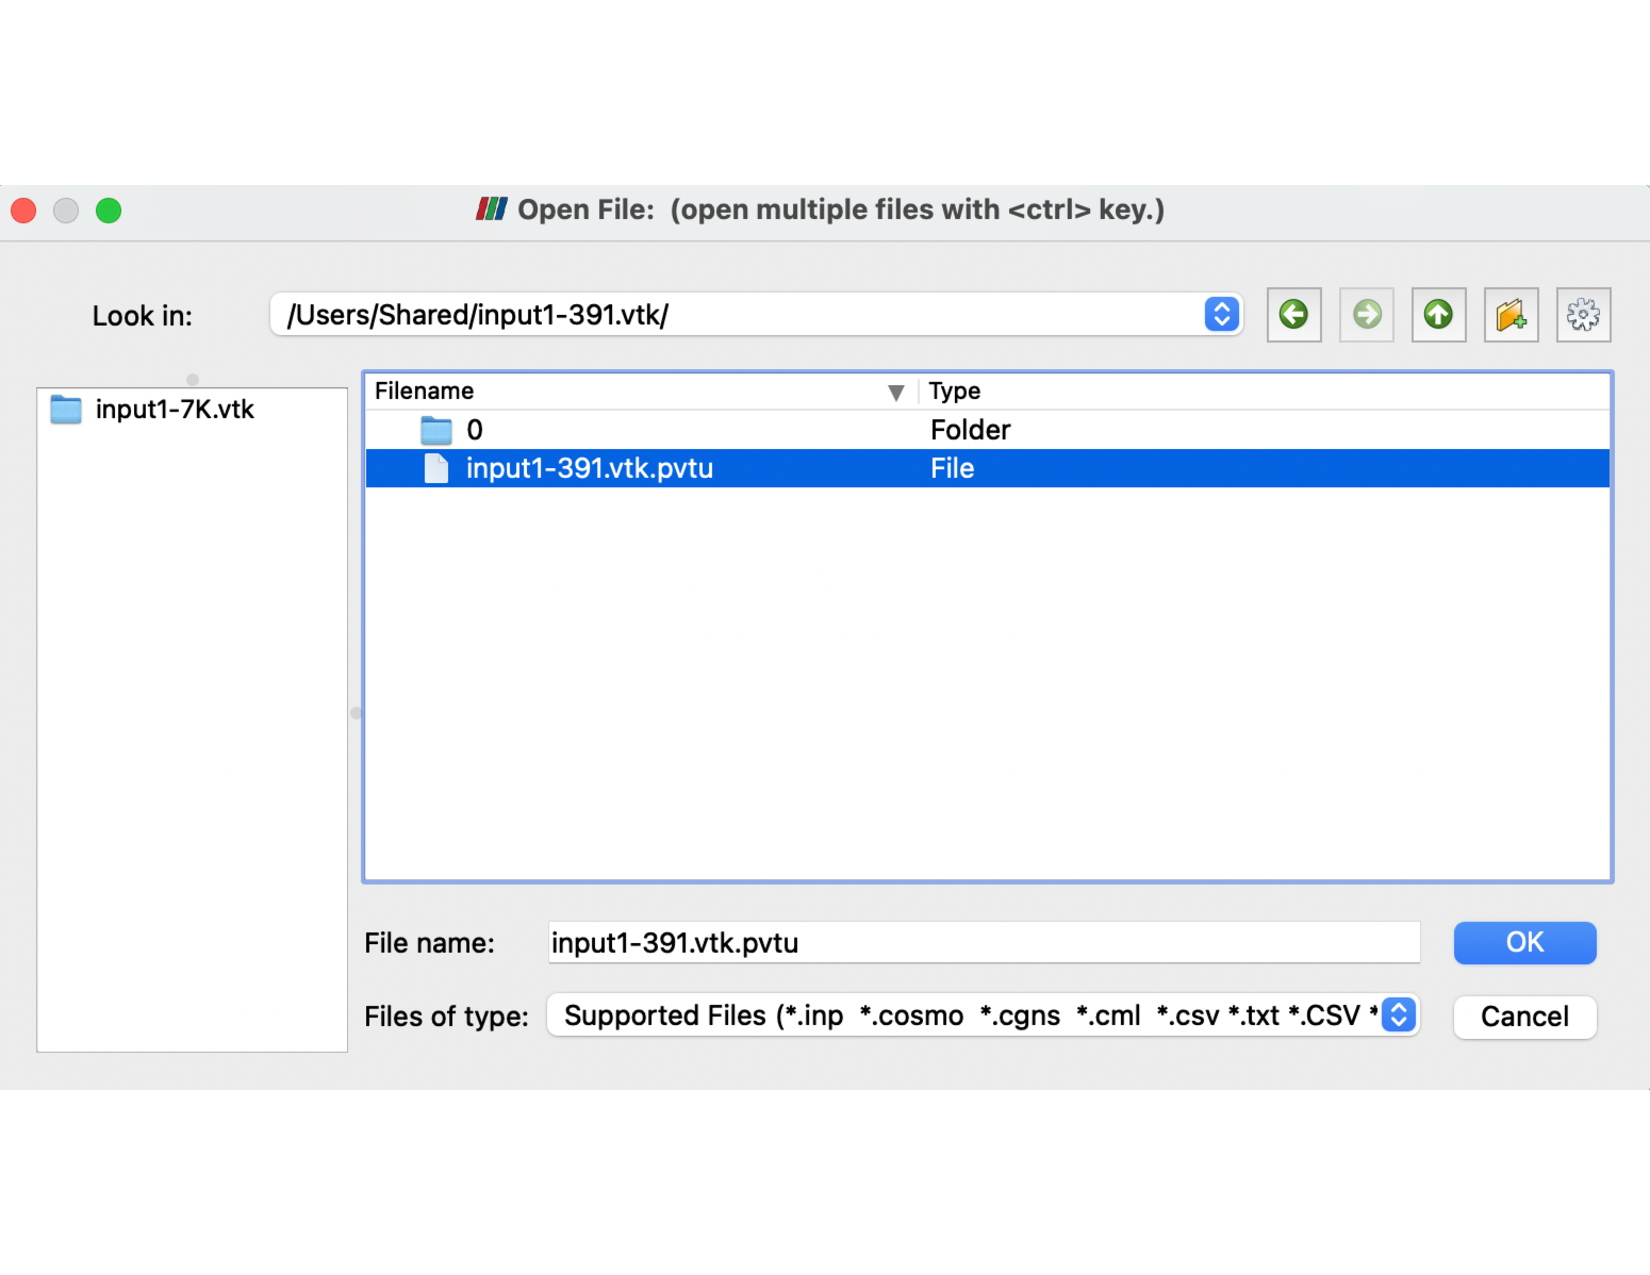
\includegraphics[width=3in]{./figures/paraview-fig1.pdf}
\caption{To visualize a mesh, select .pvtu file from Open File menu}
\label{fig:paraview-1}
\end{figure}

\begin{figure}
\centering
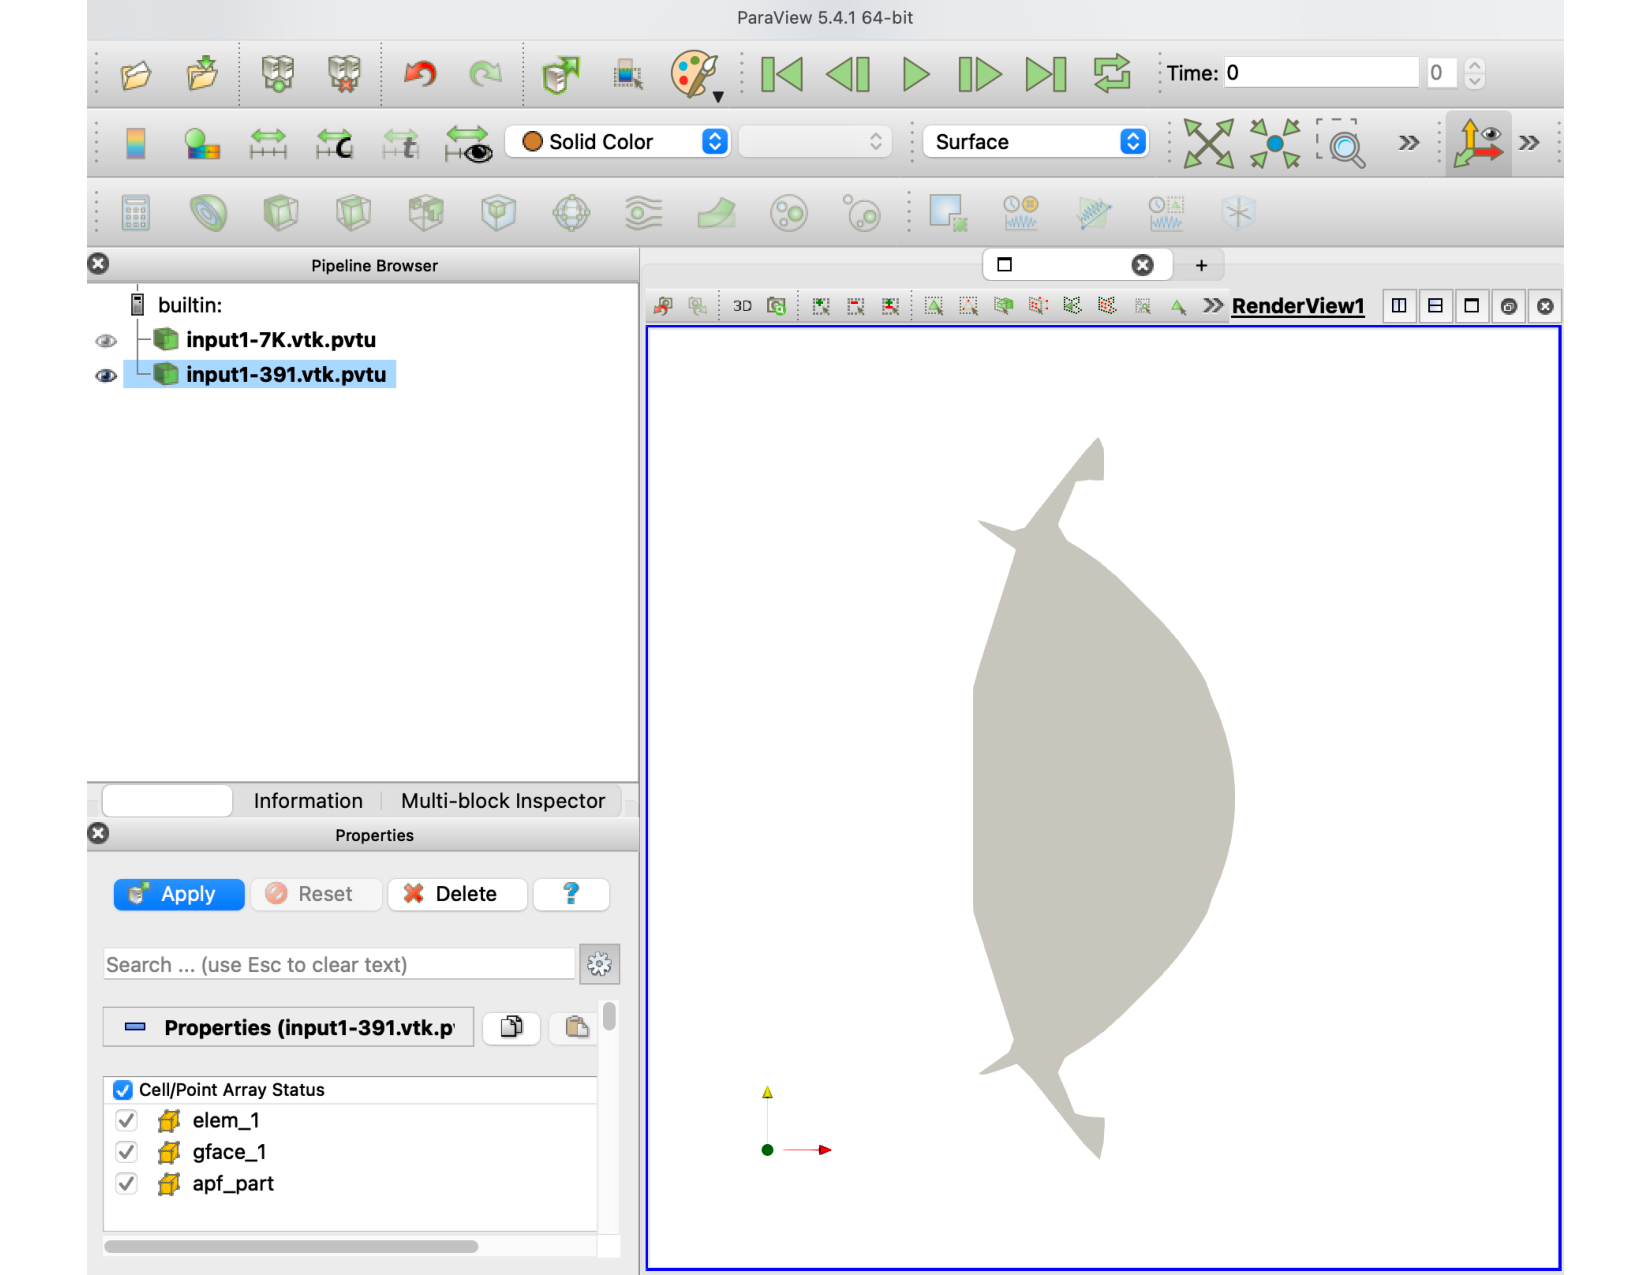
\includegraphics[width=4in]{./figures/paraview-fig2.pdf}
\caption{Initial Paraview window with a mesh}
\label{fig:paraview-2}
\end{figure}

\begin{figure}
\centering
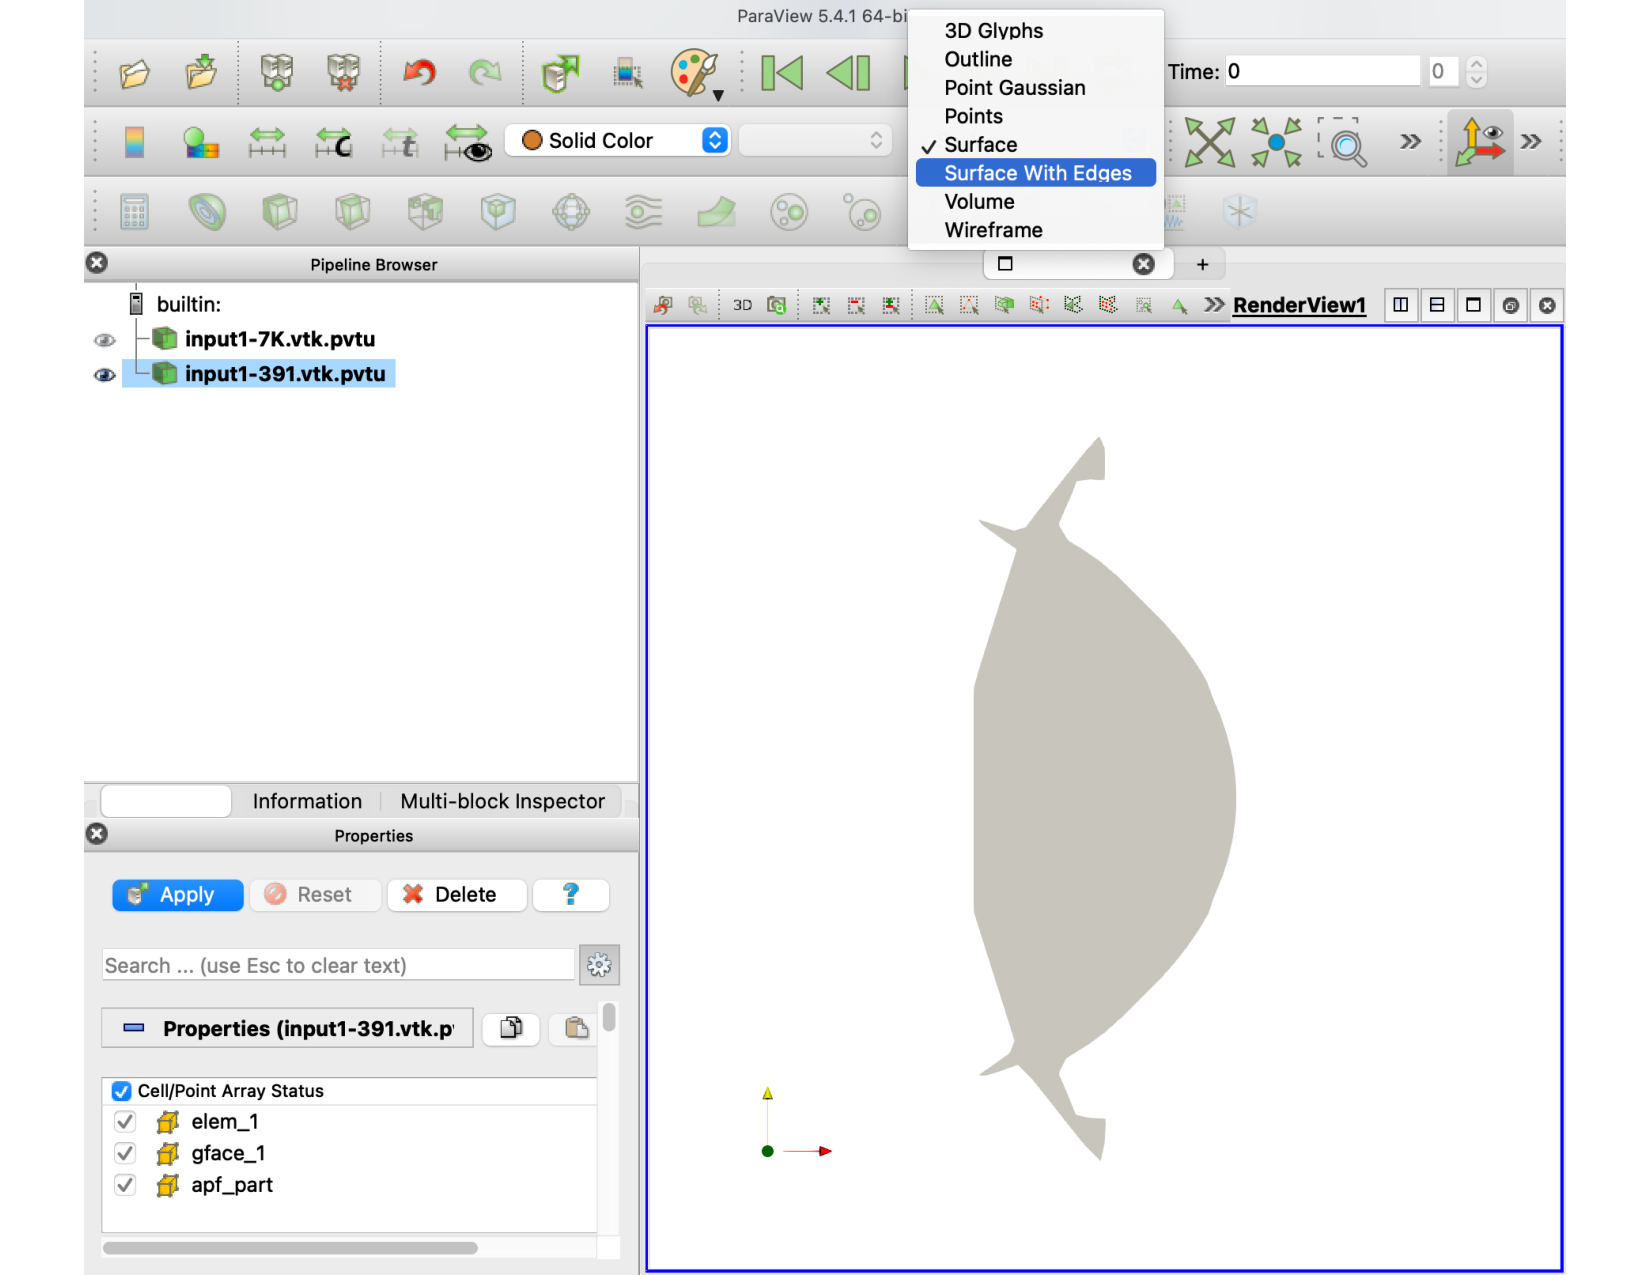
\includegraphics[width=4in]{./figures/paraview-fig3.pdf}
\caption{To render mesh decomposition, choose ``Surface With Edge"}
\label{fig:paraview-3}
\end{figure}


\begin{figure}
\centering
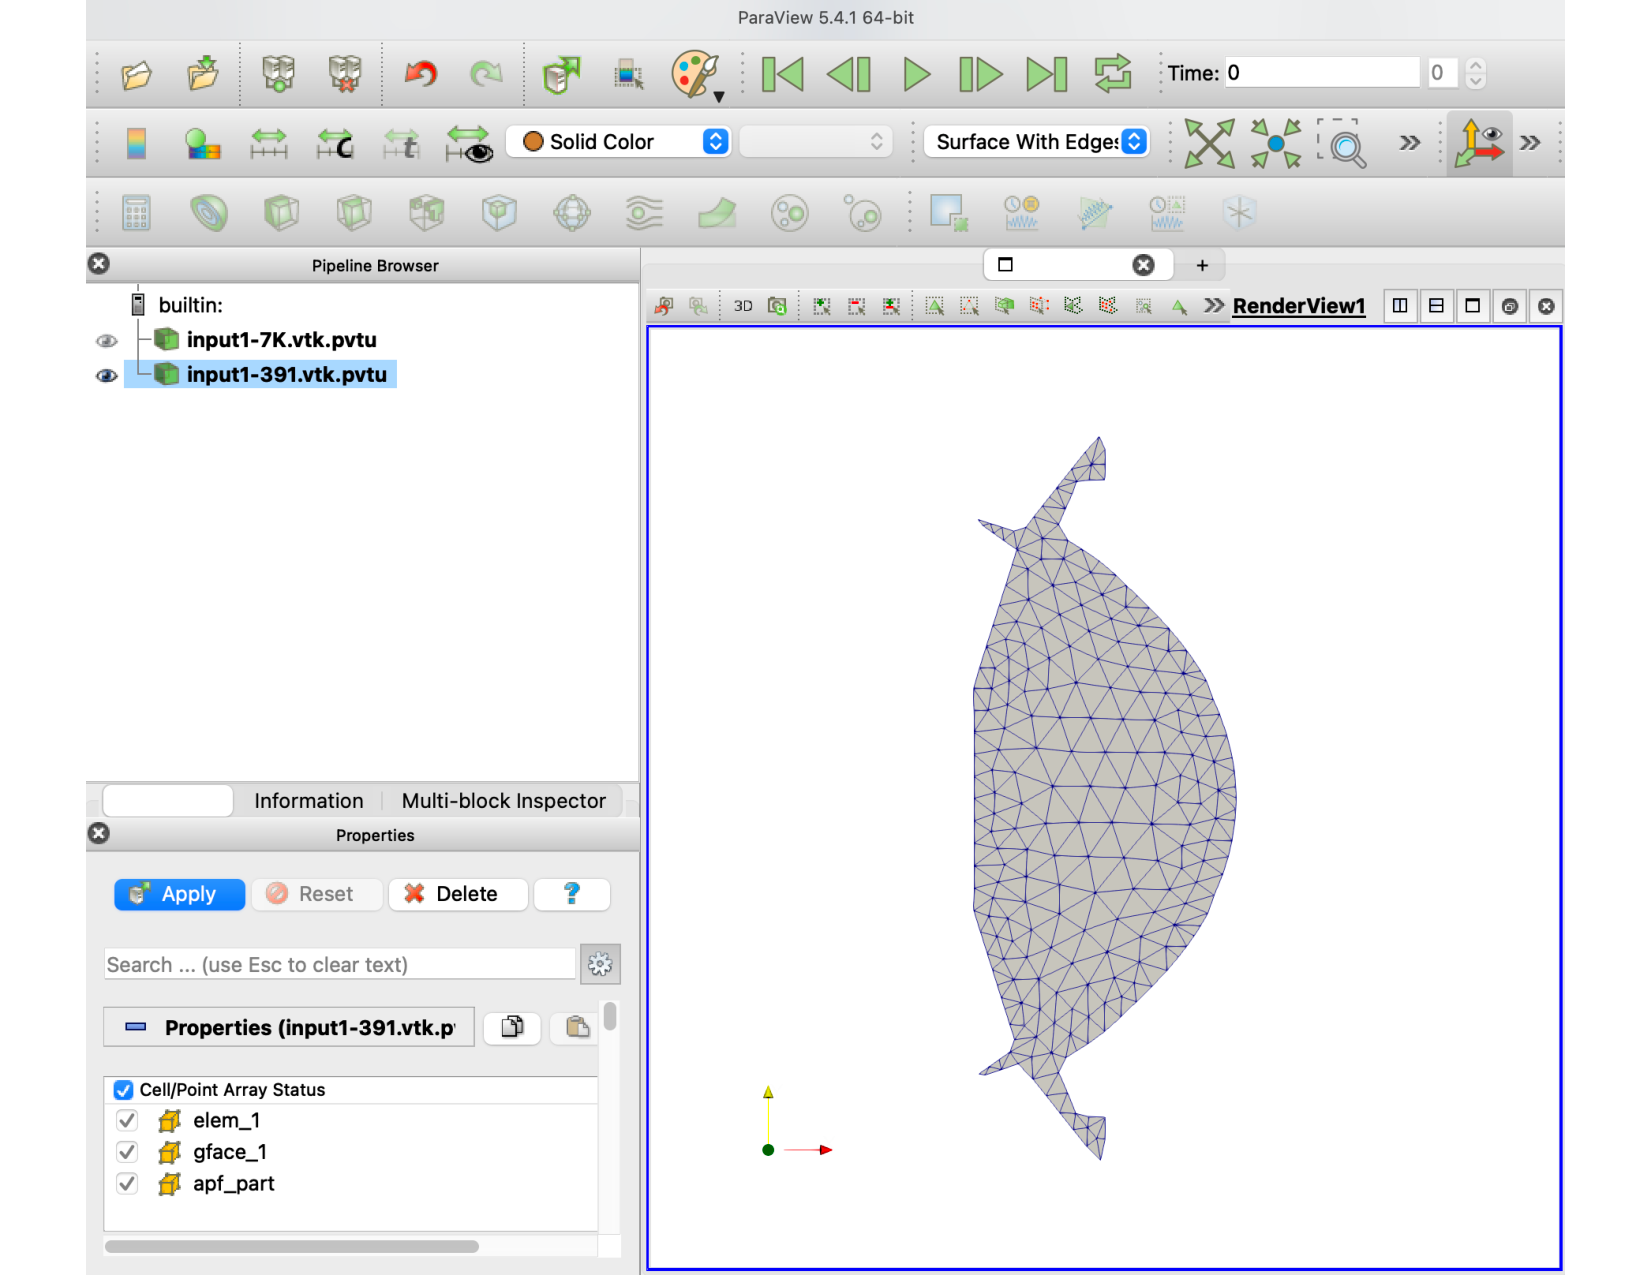
\includegraphics[width=4in]{./figures/paraview-fig4.pdf}
\caption{A mesh with ``Surface With Edge"}
\label{fig:paraview-4}
\end{figure}

If the first argument is ``output"" and the second argument is 0, filename is output, it creates the files \texttt{output.pvtu}. Opening the \texttt{output.pvtu} file in Paraview will show users the
mesh. Figures~\ref{fig:paraview-1} and ~\ref{fig:paraview-2} illustrate ``Open File" window and a mesh rendered in ``Surface" mode by default.


Changing ``Surface" to ``Surface with Edges" will outline each visible element.
Figures ~\ref{fig:paraview-3} and ~\ref{fig:paraview-4} illustrate how to make the decomposition visible.

Also, the mesh by default is rendered in one ``Solid Color".
There should be other options corresponding to the fields and numberings
that were on this mesh at the time of file writing.
There is an ``apf\_part" alternative for files written by APF, which
allows users to see the parallel partitioning of the mesh in color.

\begin{figure}
\centering
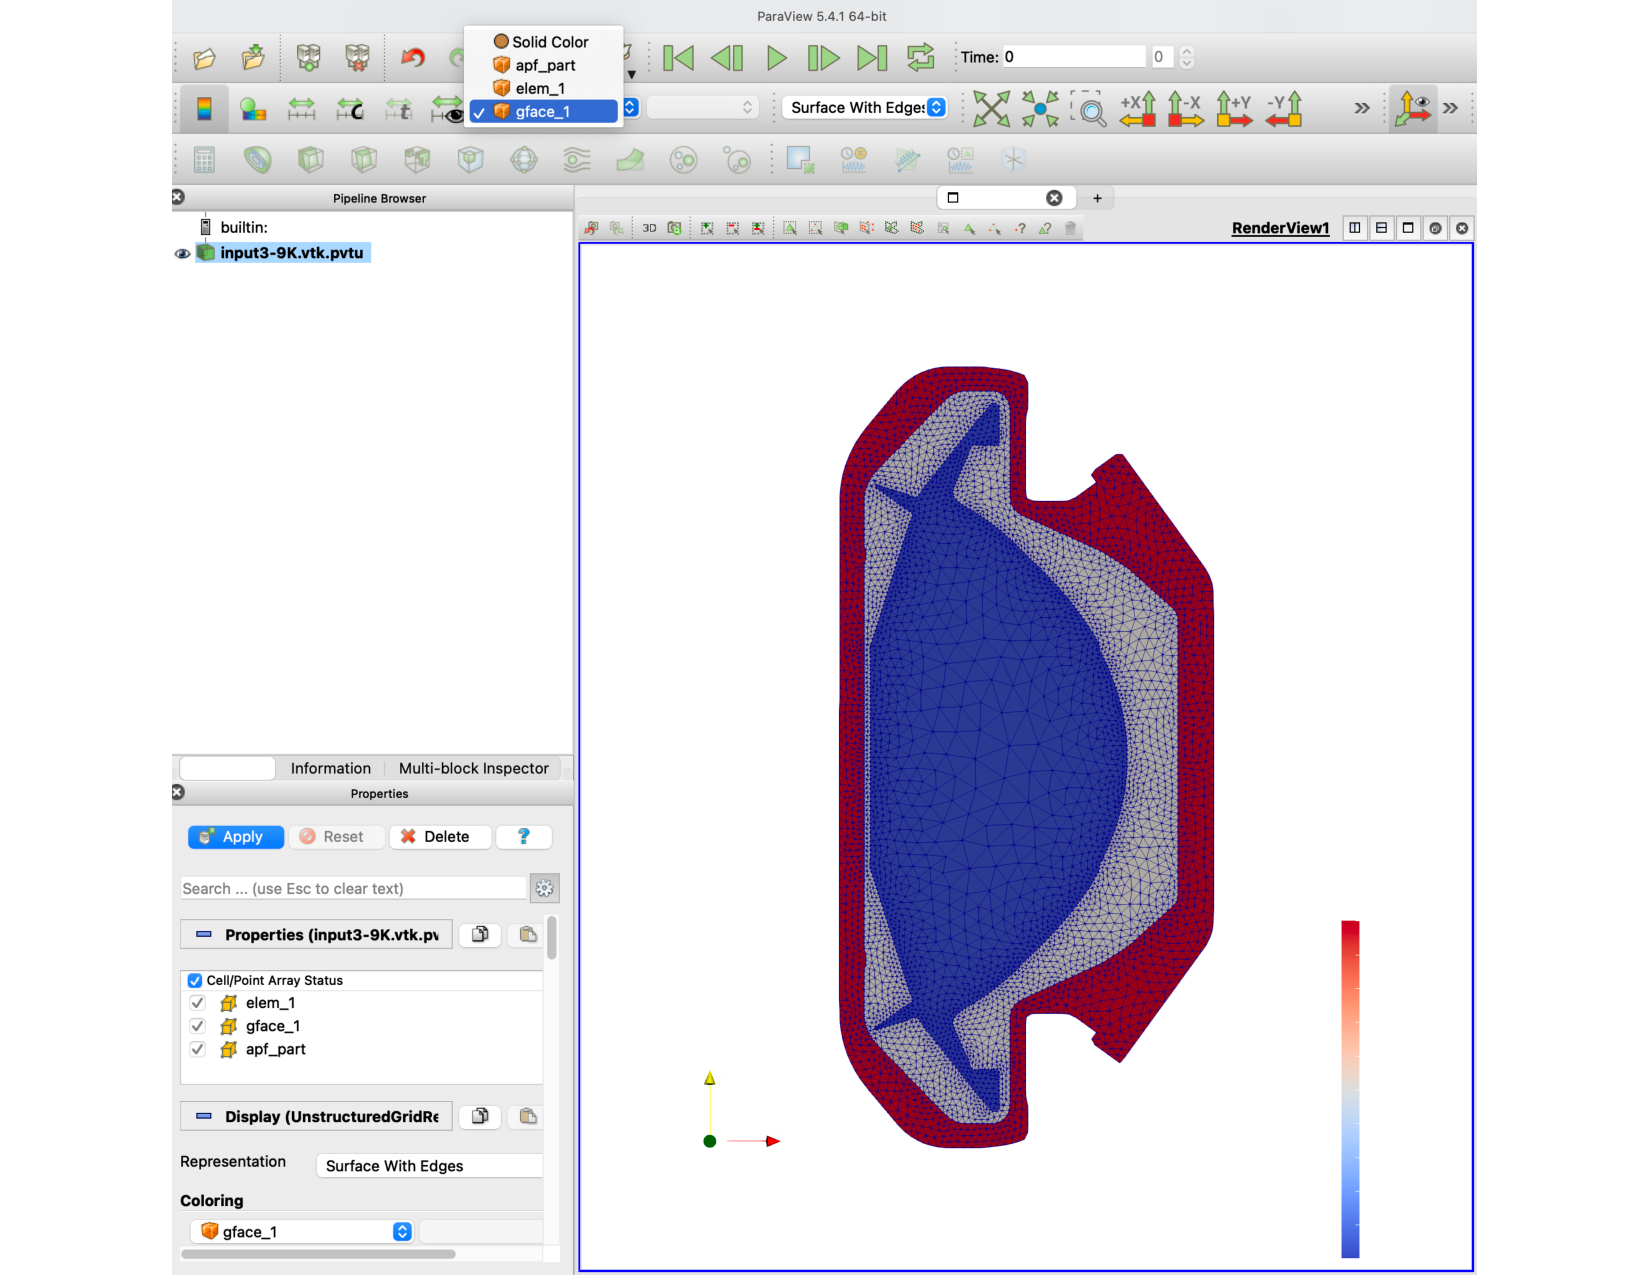
\includegraphics[width=4in]{./figures/paraview-fig5.pdf}
\caption{A mesh rendered with ``gface"}
\label{fig:paraview-5}
\end{figure}

Mesh generation program provides ``gface" alternative, which
allows users to see the geometric face of the mesh in color. 
Figure ~\ref{fig:paraview-5} depicts a Paraview window with a mesh rendered with ''gface".

\end{document}

